
\section{Introduction}
We live in an age where data is becoming the new gold. Everything is recorded, from social media interactions to online shopping habits. Every click, swipe, and purchase generates a ton of personal information. Increasingly more of life can be summarized in bits and bytes, the language of computers, making everything reducible to data. We now have AI systems like Centaur that understand human behavior better than we do ourselves, improving upon centuries of research in psychology and cognitive science, and demonstrating an unprecedented ability to predict human choices, \cite{Binz2025}. In this worldview there is a potential for optimization that is unprecedented. Whole systems including human societies can be analyzed, predicted, and even manipulated based on the data they generate. This shift towards a data-centric worldview has led to the rise of what is often referred to as "Dataism."

Dataism, a term popularized by Yuval Noah Harari in his book 'Homo Deus', refers to a concept where data is viewed as a sacred entity, almost a new religion, where algorithms and data processing are seen as the best way to understand and control the world, as they could supposedly do a better job than humans at making decisions, \cite{Harari2017}. Indeed, algorithms are increasingly being used to make decisions that were once the domain of human judgment, from hiring practices to medical diagnoses. The tech world is moving fast, and we see some overlap with this concept. With the recent rise of AI, we are today witnessing this movement in real time. Data is the new currency, and algorithms are the new priests, interpreting this data to make decisions that affect our lives in profound ways. More and more trust is placed in these algorithms, ChatGPT being a prime example, where people even use it to write their essays, code, poetry, and even confide their most personal issues, as if it were a therapist, believing it can solve all their problems better than they can.

Connected devices that collects our data, like wearables, apps, smart home device, and even 'smart tattoos' or implants, are a small fragment of this larger market that uses data to provide advices, recommendations, and predictions about our lives. They know an amount of information about use, from locations, sleep patterns to menstrual cycles, mood and sports metrics. Information that are quite personal. These devices are often seen as harmless tools at our service. And it seems like the general population remains unaware of how those devices can have a preponderant role in this shift towards a Dataistic society.

This is part of a larger debate about the implications on how we think about privacy, security, and individual agency. As data becomes the primary means of understanding, we'll need efficient ways to process and analyse it. Thus removing all the barriers like privacy, security, and individual agency, would seem like a better and faster way to reach this goal as data would flow more efficiently, allowing for faster and more accurate decision-making. 

This paper thus explores the implications of this shift towards a Dataistic society, focusing on the role of connected devices in shaping our understanding of privacy, security, and individual agency. It examines different aspects of it, and explores what solutions we might adopt if we wish to avoid living in a dystopian society where our data is used to make decisions about us without our consent or understanding. For example, wearables could become trackers that monitor our every move, thought, emotion, interaction, chemical reaction, and conversations. What you eat, who you connect to, what career path to follow, and which partner to choose, could be determined by algorithms designed to optimize our lives for the common good. No privacy just transparency, where humans would just be data points in a larger system where emotion would be understood and predicted. Natural selection would be replaced by data selection, where the most efficient human would be allowed to reproduce, and the rest would just be marginalized.

Of course, this is an extreme example, and it is not here to nourish fear, but to be aware of it. This is not going to come from one day to the other. It is a very slow and gradual process, that is already happening, but we do not realize it or do not really care yet. And as small change compounds, it can lead to a very different society in the future. What legacy do we want to leave for the next generations? 

This paper is thus more focused on privacy and security as I believe they are central to moving instead towards a more harmonious world where data ownership would be more decentralized and where individuals would have greater control over their data. It explores new technologies and frameworks that could help us achieve this goal and how a sample of the population perceives them. The focus is also on wearables and how they could be used to enhance our lives and help society flourish. Where data would be used to improve our lives, and amplify our creativity, not to control us. A world that values human experience and meaning, and provides equitable access for a healthier, coexisting society.

\paragraph{Positioning of Dataism.} \textit{Dataism} is used in this thesis as a guiding framework, not as a construct that is directly tested or measured. As outline by Harari \cite{Harari2017} and critiques of datafication \cite{VanDijck2014}, it reflects a cultural trend where ongoing data extraction is normalized as a way to optimize systems. Given that the survey was not designed to measure acceptance of Dataist claims and no psychometric scale for 'Dataism orientation' was developed, the thesis focuses on measurable user attitudes like privacy concern, control preference, trust, and adoption intent. Dataism is used as a contextual framework to interpret the prominence of control and sovereignty issues in the wearables domain. The claims focus solely on observed attitudes, without drawing causal conclusions about support for or rejection of Dataism.

\section{Literature Review}
\subsection{Ethical Responsibilities and Deontological Perspectives}
This section explores the moral duty and responsibility of corporations in handling personal data collected from wearables.
	\subsubsection{Dataism as a New Paradigm and Its Impact on Agency}

	Human agency, a term that refers to the capacity of individuals to act on their own, independently, and make their own choices, is being challenged by the rise of Dataism. This raises ethical dilemmas about how we should treat individuals in a world where data is seen as the ultimate authority.
	Dataism has quietly changed how we think about control and responsibility with our devices. 
	In this new mindset, collecting and processing data is seen as more important than what people decide for themselves \cite{Harari2017}. Data becomes the main way to measure value. This can be observe through our daily lives, where we are constantly asked to share personal information with no real choice if we want to use the service or not. It has become quite the norm to gather all sorts of personal data, with companies and even governments pushing for it.

	\cite{VanDijck2014} notes, normalization gradually takes away individual autonomy. People are often encouraged to give up privacy for convenience, but they might not really understand what they’re giving up. There’s a belief that data is always fair and true, but that’s not always right. The way data is collected and used depends on what companies or governments want, and on what the tech can actually do. Because of this, being watched or tracked is just part of life now, and it’s hard to know when you’re sharing info by choice or when it’s just happening in the background. Companies and governments say they need to watch people for safety or to make things work better, but what really happens is that people lose control and big organizations get more power.

	Building on this, \cite{deOliveira2022} shows that emerging technologies like smart tattoos and other wearables effectively turn the human body into a continuous source of data. 
	What begins as health data can be flipped into marketing or political profiling, further blurring the lines between personal well-being and systemic exploitation. Neuralink \cite{Musk2019} is also another, maybe more common example, we can use to illustrate this point.
	\cite{Liu2025} introduces the concept of “datafied enhancement,” where digital technologies do more than just assist individuals: they create digital representations that may not accurately reflect the person. This brings up big questions about how much control people have and whether their privacy is being taken away, since it can be hard to know or manage what happens to their data. 

	From an ethics point of view, these changes go against the old  Kantian idea that people should be treated as ends in themselves, not just as a way to make money or serve a system. But in the current data economy, people are often just seen as numbers, and their freedom to choose is pushed aside so that companies or platforms can benefit from it.
	\subsubsection{Privacy Risks and Surveillance in Wearable Technologies}

	As wearables becomes more and more mainstream, we can come to think that actors in the digital ecosystem have a moral duty to protect use privacy and autonomy. This constant, often passive, collection of data means that many users remain unaware of the amount of personal information their devices are transmitting. What happens to those data, who gets access, how it’s used, and for what reasons. Indeed, wearables are constantly tracking metrics like heart rate, sleep, location, menstrual cycle and even mood. This data is often sent to servers run by third parties, sometimes in other countries, and users are rarely told exactly what’s happening \cite{Sui2023}. When things aren’t clear, trust suffers—and real consent becomes unlikely, which is a recurring challenge in the governance of wearable technologies.

	Data collected for one purpose today can easily be reused for another purpose tomorrow. For example, companies might say they’re gathering health data to help users improve their well-being, but that same data can be instead used for targeted ads or even political profiling. The Cambridge analytica scandal, where personal data was used to influence political opinions and elections \cite{Kanakia2019}, showed this point clearly. \cite{deOliveira2022} points that once biometric data is collected, it tends to become a commodity, a marketable asset, traded or used in ways most people never thought off. 

	There are also technical risks to consider. Wearables can be hacked or breached, and even with security measures in place, there are still vulnerabilities, especially if users don’t have real control over their own data.

	Social norms and institutional habits complicate things further. As wearables become more common, the idea of “normal” data sharing keeps expanding. The promise of better health or convenience can make people overlook the risks of giving up so much information.\cite{VanDijck2014} notes that data from wearables is now treated almost like currency, exchanged for access to services. But these exchanges are rarely clear, and users often don’t realize how much control they’re giving up. Over time, this can leave people feeling less in charge of their digital lives, as they become more like data sources than active participants.

	Consent is another tricky area. Indeed, many platforms rely on broad, one-time agreements that don’t really fit the ongoing, ever-changing nature of wearable data collection. What’s needed are more flexible, context-aware ways for users to decide what they’re comfortable sharing ~\cite{Riso2017}.

	In the end, the privacy and surveillance issues tied to wearables are complicated and deeply rooted in how our society now treats data. This won't be solve by tech alone. It demands a serious review of the social, ethical, and legal rules around data. Only by combining strong security, clear data practices, and real user empowerment can we hope to reduce the risks and get the most out of wearable technology without sacrificing privacy and autonomy.
	\subsubsection{Ethical and Regulatory Frameworks for Data Governance}

	The rapid evolution of wearable technologies has exposed significant gaps in the ethical and regulatory frameworks that are supposed to protect users’ rights and interests. As the literature shows, the legal landscape has struggled to keep pace with the technical innovations and the new forms of data collection that characterize the age of Dataism. Bouderhem~\cite{Bouderhem2023} points out that regulations like the GDPR (General Data Protection Regulation), a comprehensive data protection law in the European Union, and the EU Data Act have set important standards for data protection. But in practice, they often lag behind, react too late and are fragmented in practice, thus struggling to keep pace with innovation. The complexity of wearable data, its sensitivity, its volume, and the diversity of actors involved, means that traditional compliance-based approaches are not enough. The literature highlights the need for more robust technical safeguards, such as end-to-end encryption and AI-based monitoring, but also for regulatory mechanisms that can adapt to the fast-changing environment of digital health. Riso et al.~\cite{Riso2017} propose a framework of six core ethical values: scientific value, user protection, agency, trustworthiness, benefit, and sustainability, that should guide the responsible sharing of personal health data. However, in practice, there are significant gaps between these ethical ideals and the way platforms actually operate. The challenges of trust, transparency, and user empowerment are discussed in detail in subsequent sections.

	In addition, collaboration between stakeholders emerges as very important in the literature. Sui et al.~\cite{Sui2023} argue that effective governance of wearable data cannot be achieved by companies or regulators acting alone. Instead, there is a need for participatory approaches that involve users, developers, researchers, and civil society organizations in the design and oversight of data systems. This collaborative model is seen as essential for building privacy safeguards into the architecture of wearable technologies from the outset, rather than treating them as an afterthought. By involving users in the design process, companies can better align their practices with ethical principles and societal expectations, reducing the risk of backlash or regulatory intervention. However,this is not easy. The literature points to several challenges, including the global nature of data flows, the diversity of legal regimes, and the technical complexity of implementing user-centric controls. Bouderhem~\cite{Bouderhem2023} notes that even the most advanced regulations can be undermined by loopholes, inconsistent enforcement, or the rapid emergence of new technologies that fall outside existing legal definitions. Moreover, even careful rules can slow innovation or raise entry barriers, reinforcing the dominance of established large players.

	In summary, the ethical and regulatory frameworks for data governance in wearable technologies face many challenges.The literature reviewed here makes it clear that adjustments to existing laws and practices will not be enough to address the challenges posed by Dataism and the centralization of data power. What is needed, is a large-scale, integrated approach with strong technical safeguardsm adaptive regulation and true user agency.
	Only by rethinking the foundations of data governance, placing ethical values and user rights at the center, can we ensure that wearable technologies serve the interests of individuals and society, rather than simply reinforcing the 
	power of corporations or data aggregators. But as \cite{Aghion2021} argue that the regulations designed to protect workers can also slow down innovation, a paradox. This highlights the need for a balanced approach that recognizes the importance of both ethical imperatives and the practical realities of fostering innovation.
	\subsubsection{Technical and Practical Challenges: Quality, Interoperability, and Consent}

	Data collectors have a duty to ensure the data they collect is accurate, interoperable, and managed with meaningful user consent. Failing to address these technical challenges means failing in their moral responsibility to protect users. These challenges are persistent and complex. As wearables become more set in daily routines, the question of how to ensure data quality, interoperability, and meaningful consent becomes important to this debate.

	A first and recurring issue is data quality. Wearable devices, despite their promise of continuous and personalized health monitoring, often produce data that is inconsistent, incomplete, or biased. \cite{Canali2022} highlight that sensor variability, device calibration, and environmental factors can all affect the reliability of the data collected. Inaccurate or low-quality data can lead to false positives, overestimations of health risks, or even missed diagnoses. The consequences are technical but also ethical, as users may make decisions based on flawed information, and healthcare providers may lose trust in the systems. The literature ~\cite{Canali2022} suggests that establishing local quality standards and regular validation protocols is needed, but the fragmented nature of the wearable market makes this difficult to enforce. Without standardized benchmarks, comparing data across devices or integrating it into clinical workflows remains a challenge.


	Interoperability is another challenge. The wearable tech landscape is scattered across countless proprietary systems (a way that companies lock users into their ecosystems), locked-down data formats (a way that companies restricts how data is stored and accessed), and isolated communication protocols (a way that companies limit how devices talk to each other). This fragmentation makes it difficult for users to aggregate their data or for healthcare providers to access comprehensive records. Canali et al.~\cite{Canali2022} and Bouderhem~\cite{Bouderhem2023} show that interoperability gaps not only hurt the utility of wearables but also reinforce the dominance of large platforms that can dictate the terms of data exchange. The absence of common standards also complicates regulatory oversight and limits the potential for decentralized solutions, such as personal data vaults or blockchain-based systems, to be integrated into existing infrastructures \cite{Mun2010}. The literature calls for coordinated efforts among manufacturers, regulators, and standards bodies to develop interoperable frameworks.

	Consent is also a practical challenge in the context of wearables. We detailed it later in the Transparency \& Informed Consent section, but traditional broad one-time consent models are inadequate for continuous data flows and shifting purposes.

	Security is another layer that cannot be ignored. Indeed, the aggregation of sensitive health data in real time creates attractive targets for malicious actors. Even when companies implement encryption and other security measures, breaches and unauthorized access remain common, as highlighted by \cite{Mone2023}. The complexity of wearable ecosystems, where data may pass through multiple devices, apps, and cloud services, increases the attack surface and makes it difficult to ensure end-to-end protection. Bouderhem~\cite{Bouderhem2023} suggests that AI-based monitoring and real-time anomaly detection could offer new safeguards, but these solutions introduce their own challenges, such as algorithmic transparency and the risk of false alarms.

	The push to collect, process, and use more data, part of the Dataism paradigm, creates new technical dilemma and raises new ethical duties for the main actors. They have a duty to ensure the data they collect is accurate, interoperable, and managed with meaningful user consent. Failing to address these technical challenges means failing in their moral responsibility to protect users. But technical and practical challenges of quality, interoperability, and consent in wearable data governance are complex and mixed with broader issues of power, trust, and user autonomy. Addressing these challenges requires technical innovation but also a commitment to transparency, standardization, and user empowerment. If those issues are addressed ethically, wearables might be able to deliver on the health gains without giving up rights and freedoms.
\subsection{Digital Sovereignty and Consumer Empowerment}
	\subsubsection{Data Ownership \& User Control}

	When it comes to wearables, the question of data ownership and user control is important in the context of digital sovereignty. In a world shaped by dataism, where data is seen as the ultimate authority, the question of ownership over the data generated by our bodies takes on a new dimension. It goes beyond technical or legal issue to become political and philosophical. The literature shows that, despite the promises of empowerment and autonomy, the reality for most users is still far from true ownership or meaningful control.

	What stands out in the literature is how the concept of “ownership” is often used in a very ambiguous way. \cite{Hummel2021} show that data sovereignty can mean legal rights, technical control, or even just the ability to manage data in practice. This ambiguity directly shapes how organizations structure their platforms and how individuals experience their rights. In the context of wearables, this ambiguity is even more problematic because the data is so personal and continuous. If ownership is not clearly defined, it is easy for platforms to claim that users “own” their data while still locking them into closed ecosystems where they cannot actually do much with it.

	\cite{Safavi2014} try to address this by proposing a privacy framework with ten principles, including ownership, transparency, and modifiability. Their ninth principle, “Ownership,” is especially relevant here: it says that data ownership should be fully transparent and granted solely to the user. In theory, this sounds like a strong foundation for user empowerment. But in practice, as the authors themselves point out, most commercial wearables do not implement these principles. Data is collected and stored in a file format owned and controlled by a specific company (proprietary format), and users are often given only superficial access, \cite{Canali2022}, like a dashboard or a download button, but not the ability to truly control, delete, or transfer their data as they wish. The framework also includes practical checklists, like secure communication lines and user management, but these are rarely adopted by the big players in the industry.

	This gap between theory and practice is analyzed by \cite{Conradie2022} who argue that the lack of meaningful user control is a direct result of the dataist business models that dominate the wearable ecosystem. Data is treated as a commodity, and the incentives are structured so that companies benefit from collecting as much as possible, often at the expense of user autonomy. The moment the data leaves the device, users lose almost all control over what happens next. According to the authors, a more distributed model where sharing control among users, manufacturers, and regulators through a distributed model would be beneficial. That said, they admit that this would require big changes in both technology and governance, and that current regulations and attitudes are not yet ready for such a shift.

	The real-world consequences of this situation are visible in consumer attitudes. \cite{Arbanas2023} report that trust in companies is falling, and that users are increasingly demanding the right to see, control, and delete their data. Many feel that no matter what actions they take, companies or hackers will still be able to get to their data. This sense of disempowerment is backed by the structure of most wearable platforms, which are designed to maximize data extraction and minimize user intervention. More on consumer behavior is discussed in the section "Behavioral Science and User Decision-Making". Many examples in the literature show how data collected for one purpose is repurposed for another, often without clear consent or oversight ~\cite{Sui2023}. This only reinforces the perception that users are not really in control, even if the marketing says otherwise.

	To sum up, user empowerment is far from being a reality in the wearable data ecosystem. The ambiguity of data ownership, the lack of meaningful control mechanisms, and the dominance of dataist business models all contribute to a situation where users are often left in the dark about what happens to their data. Making this ideals a reality is far more complex than just saying 'users own their data'. It takes clear definitions, strong technical and legal mechanisms, and a fresh look at the incentives that currently shape the wearable data ecosystem. Without these changes, the promise of user empowerment will remain largely rhetorical, and the risks of centralized data power will continue to grow.
	\subsubsection{Transparency \& Informed Consent}

	When it comes to wearables, transparency and informed consent are often seen as the foundation of ethical data governance. But the reality, as the literature shows, is far more complicated. The promise is that users will know what happens to their data and will be able to make informed decisions, but the gap between what is claimed and what is actually delivered is visible, and it is precisely this gap that undermines both trust and the very idea of digital sovereignty.

	\cite{Safavi2014} put transparency at the center of their privacy framework, making it one of the ten core principles for wearable health devices. They argue that users should always be able to see what data is collected, how it is processed, and who can access it. Their checklist for modifiability and transparency is supposed to guarantee that users can adjust their privacy settings as their preferences evolve. On paper, this sounds like a good foundation for user empowerment. However, the reality is that most commercial platforms only pay small attention to these principles. Interfaces are often confusing, information is buried in lengthy terms and conditions, and the actual flows of data remain opaque for the average user \cite{Sui2023}. The result is that transparency becomes more of a marketing slogan than something real.

	The issue of informed consent is closely tied to this lack of transparency. As discussed in the section on regulatory frameworks, current laws such as HIPAA often fail to adequately protect users of wearable technologies, especially when data is handled by entities not covered by these regulations, \cite{Banerjee2018}. This leaves users with little legal protection and makes truly informed consent difficult to achieve in practice.

	This disconnection between theory and practice has real psychological and behavioral consequences. \cite{Arbanas2023} highlight that lack of transparency is a major driver of consumer distrust. Their survey data show that users want clear, enforceable rules about data use, and they are increasingly distrustful of companies that fail to provide them. There is a great psychological impact to it, as when users feel informed and in control, they are more likely to engage with digital health technologies and to benefit from them. On the other hand, opacity and complexity can lead to disengagement or even outright rejection of wearable devices.

	The literature suggests that achieving meaningful transparency and informed consent requires much more than legal compliance or technical fixes, ~\cite{Safavi2014}. It demands a shift in design philosophy towards user-centricity. Users need interfaces that are clear and intuitive, with privacy settings that are easy to locate and adjust. Companies also need to keep users informed about data practices over time, not just at the moment of purchase. Consent mechanisms must be granular and revocable, allowing users to change their minds as circumstances evolve. This is especially important in the context of wearables, where data flows are continuous and the purposes for which data is used can shift over time.

	One recurring problem is that traditional models of consent are simply not fit for purpose in the age of Dataism. The old approach where users agree to a broad set of terms once and for all does not reflect the dynamic and complex nature of data collection in connected devices. ~\cite{Safavi2014} calls for more dynamic, context-aware consent models, where users can adjust permissions in real time and are kept informed about how their data is being used.

	It is also worth noting that transparency and informed consent are about enabling genuine agency. When users understand what is happening with their data and can make meaningful choices, they are more likely to trust the system and to participate actively in it. This, in turn, can drive innovation and improve outcomes for everyone. But as long as transparency remains superficial and consent is reduced to a formality, the promise of digital sovereignty will remain unfulfilled.

	Dataism’s normalization of data collection has eroded user agency and made privacy trade-offs routine.
	Transparency and informed consent are thus essential for digital sovereignty and consumer empowerment, but without real transparency and dynamic, revocable consent, users cannot be empowered or in control of their data. A fundamental rethinking of how companies communicate with users and design their systems needs to happen in order to move towards a model where users are truly in control of their data, rather than passive subjects in a data-driven economy.
	\subsubsection{Technical Privacy \& Security Safeguards}

	Privacy and security safeguards are essential for any serious approach to digital sovereignty, especially when it comes to wearables. But as the literature shows, the reality is more complex than simply deploying encryption or creating technical features. How they are implemented, integrated, and how they actually empower users rather than just protecting data in the abstract is what matters.

	\cite{Abouelmehdi2018} provide a useful starting point by comparing anonymization and encryption techniques for healthcare data. Their analysis is quite comprehensive, showing none of those methods dominates the other. Anonymization, for example, is supposed to remove personal identifiers, but in practice, re-identification attacks are still possible, especially when datasets are combined. Encryption, on the other hand, is only as strong as its key management and the security of the endpoints. The authors note that combining both methods can improve protection, but it also increases complexity and computational technicity. This is particularly relevant for wearables, where devices are often resource-constrained and users expect seamless experiences.

	\cite{Safavi2014} privacy framework, cited in the previous section, takes a more holistic approach. Their ten principles and nine practical checklists merge privacy and security into the design of wearable health devices from the bottom up. Principles like secure communication lines, access control, and auditability are complemented by requirements for user-friendly interfaces and transparency. What stands out is the emphasis on usability: security measures should not make the device harder to use, otherwise users will simply bypass them or abandon the product. As the literature shows, technical safeguards only work if they are easy to access and understand for the people they aim to protect.

	The challenge, however, is that those frameworks are good for academia, but the reality is that most commercial platforms do not fully implement these frameworks, \cite{Arbanas2023}. There is often a gap between what is technically possible and what is actually deployed in the market. \cite{Conradie2022} argue that robust security is a prerequisite for digital sovereignty, but they also point out that weak protections are still common, exposing users to exploitation and undermining trust. The business incentives are not always aligned with user empowerment: companies may prioritize speed to market or cost savings over comprehensive security, especially if users are not demanding more.

	\cite{Hummel2021} add another layer by discussing technical management strategies as part of a broader approach to sovereignty. Strong cryptography, secure storage, and access controls are necessary, but not sufficient. The authors argue that technical safeguards must be integrated with legal and organizational measures, and that users need to be aware of how these systems work in practice. Otherwise, security becomes a black box, something that happens in the background, but does not actually give users more control or understanding.

	Another key takeaway from the literature is the need for continuous adaptations, \cite{Bouderhem2023}. Threats evolve quickly, and what is considered secure today may be obsolete tomorrow. In the context of wearables, where new devices, apps, and integrations are constantly being released, security measures need to be updated regularly, and companies must be proactive in monitoring for vulnerabilities and responding to incidents, \cite{Mone2023}. This is complex and requires strong technical expertise, but also organizational commitment and regulatory oversight.

	Finally, it is important to recognize that technical safeguards alone are not enough. They must be part of a broader ecosystem that includes transparent communication, user education, and responsive governance. Users need to understand what protections are in place, how to use them, and what to do if something goes wrong, \cite{Cilliers2019}. Otherwise, even the best technical solutions will fail to deliver real empowerment or trust.

	Centralized model have normalized privacy trade-offs and diminished user agency, \cite{Cilliers2019}. Technical privacy and security safeguards are essential for digital sovereignty, but they need to be complemented. Usability, education and responsive governance are also needed to move towards a model where users are not just protected, but genuinely empowered to control their data.
	\subsubsection{Regulatory Frameworks \& Accountability}

	Building on the earlier section, we move to the concrete gaps. Accountability, enforcement, and regulation will be the main focus.

	\cite{Banerjee2018} critique of the current state of regulation was made using the HIPAA Partnership-Identity they created. It is an 'Exposure Matrix' to show how existing laws often fail to address the specific risks posed by wearables. They found that the highest danger zone occur when identifiable health data is handled by non-covered entities (entities not subject to HIPAA’s protections). In these cases, users have little legal power if their data is misused or breached. The authors say that the law has not kept pace with the realities of continuous, granular data collection and sharing. They call for legislative updates that reflect the new dynamics of wearable data, including more robust requirements for transparency and user consent.

	\cite{Conradie2022} dive deeper, pointing out that the gaps take root from structural power imbalances in the digital ecosystem. They argue that current frameworks often prioritize the interests of manufacturers and service providers over those of users. This is especially problematic in the context of digital sovereignty, where the goal should be to empower individuals to control their own data. The authors advocate for reforms that clarify data ownership, mandate user-centric controls, and establish clear lines of accountability. Without these, the promise of digital sovereignty will just be empty words.

	\cite{Hummel2021} show how legal definitions are not consistent across jurisdictions. Their review of over 300 publications shows that terms like “data sovereignty” and “digital sovereignty” are used in different ways depending on the legal, technical, or cultural context. This lack of harmonization creates confusion for both users and companies, especially as data often crosses borders. The authors suggest for more consistent, harmonized policies that support both individual rights and the realities of cross-border data flows.

	From a consumer point of view, \cite{Arbanas2023} highlight the growing demand for stronger government oversight and corporate accountability. Their survey data show that trust in companies is declining, and that users want clear rules about data use, the right to see and delete their data, and meaningful consequences for misuse or breaches. 
	Self-regulation, where companies set their own rules, has not been sufficient to protect users. Instead, there is a call for more robust government intervention, including independent audits, clear penalties for violations, and mechanisms for users to seek compensation when their rights are violated.

	A repeated theme is that regulation fail in a moving environment. Static laws quickly become outdated in a field where new devices, data types, and business models are constantly emerging. The literature points to the need for regulatory frameworks that are flexible, inclusive, and capable of evolving alongside technology. This includes not only updating existing laws but also creating new forms of oversight that involve users, civil society, and technical experts in the regulatory process. Models that bring users, civil society, and experts into rule-making surface is presented as a practical path forward, \cite{Sui2023}.

	Equally important is the balance between industry self regulation and hard law. While industry codes and best practices can help set standards, they are often voluntary and lack real enforcement power. Consensus leans toward a hybrid model, with self-regulation plus enforceable obligations and explicit accountability. This is especially important for cross-border data flows, where national laws may conflict or leave gaps that can be exploited by less scrupulous actors.

	In summary, regulation must be thought again to prioritize user rights, transparency, and adaptive governance. Regulatory frameworks are essential for enabling a strong digital sovereignty and user empowerment. Without effective, user-centric regulation, technical safeguards and user control mechanisms cannot deliver real protection or agency. 
\subsection{Behavioral Science and User Decision-Making}
	\subsubsection{Internal Calculus}

	In the context of Dataism, users may lean towards sharing their personal information, as algorithms are increasingly seen as capable of making better decisions than humans. Privacy concerns may thus fade away in the face of perceived benefits, such as improved health outcomes or personalized services. 

	Studies on privacy calculus shows that people do not just weigh risk against reward in a simple way, \cite{Li2016}. The theory says users weigh what they hope to gain like health insight, convenience, status, against risks like misuse or loss of control. But this calculation is not always rational, and differs from person to person.

	The privacy calculus is shaped by a mix of personal, social, and contextual factors. For example, \cite{Li2016} show that people are more likely to accept privacy risks if they believe the benefits are substantial or if they trust the brand behind the device. Indeed, trust in the provider can act as a kind of shortcut in decision-making, especially when the technical details of data handling are too complex for most users to fully understand. At the same time, the perceived usefulness of the device, whether it actually helps users achieve their health goals, plays a decisive role. If a device is seen as essential or uniquely valuable, privacy concerns tend to fade away.

	Nevertheless, the calculus is not just about individual preferences. Social influence and cultural context also matter. \cite{Pentina2016} point out that personality traits like extraversion and agreeableness make people more likely to focus on the benefits of using mobile apps, even when those apps require access to sensitive information. In some cultures, the collective attitude towards technology and privacy can further tip the balance. For instance, in environments where sharing data is normalized or even encouraged, users may feel less hesitation, regardless of their own concerns. It reflects the Dataist view where more data leads to better outcomes for both people and society, \cite{Harari2017}.

	Another layer comes from demographic and psychological factors. \cite{Kordzadeh2016} found that older adults and those in better health are generally more cautious about sharing personal health information, while people with poorer health or strong emotional ties to online health communities are more willing to take risks. This suggests that the privacy calculus is not static and that it shifts depending on life circumstances and the perceived urgency of the benefits. For someone facing a serious health issue, the promise of support or improved care can outweigh even significant privacy risks.

	And despite all that, there is still a gap between what people say and what they do. That gap is the privacy paradox. Many users express concern about privacy but still go ahead and use devices or apps that collect large amounts of personal data. \cite{Sun2015} link this to immediate hedonistic pleasure. Indeed immediate enjoyment and social contact seems to feel more real that abstract privacy worries. There is also gender differences. Women react more to risk and lean more toward caution, while men tend to lean toward perceived gains. But context still frames the outcome for both.

	What complicates the picture further is the general lack of awareness about the real risks involved. Studies like \cite{Cilliers2019} and \cite{Datta2018} show that many users do not fully understand how their data is collected, processed, or potentially misused. This lack of knowledge can lead to underestimating the risks and making decisions that do not truly reflect personal preferences or values. In other words, the privacy calculus is often based on incomplete or inaccurate information, which raises questions about how meaningful these trade-offs really are.

	The way consent and controls are designed also shapes the calculus. If privacy settings are buried in complex format or written in complicated legal terms, users are more likely to accept default options without much thought \cite{Banerjee2018}. On the other hand, clear communication and user-friendly interfaces can empower users to make more informed choices. \cite{Gupta2023} show that real options like delete data, set access rule, or revoke access, make people more willing to share.

	The points above explain why users make those choices, but those trade-offs aren't accidental as Dataism frames them in some ways. Understanding these trade-offs is important for developing technologies and policies that respect user autonomy without sacrificing the potential benefits of innovation. With wearables starts to become a part of ourselves, the priority would be to shift towards a genuine informed choice.
	\subsubsection{External Pressures (Trust and Transparency)}

	Trust is fundamental for the adoption and ongoing use of wearable health technologies, yet it is also very fragile. Studies show people share because of trust in the institutions that are handling their data and less because of the tech features, \cite{Hutchings2020}. Winning that trust is tough as the lines between business, healthcare, and personal privacy now overlap.

	Healthcare professionals and public institutions are more trusted than commercial companies, \cite{Hutchings2020}. People are generally open to sharing their medical data for research or treatment if they believe the recipient is trustworthy and the purpose is clear. It changes once the the data is put into the hands of private firms, especially those built on monetizing it. Users become more reluctant to share, fearing misuse or loss of control. Under Dataism, the line between user and product thins. That's the anxiety behind turning health into a commodity.

	Transparency influences trust, \cite{Sui2023}. We already saw the gap between promised transparency versus confusing interfaces and opaque flows that erodes trust. Faced with long terms or vague policies, users are left with little choice but to take the decision to accept or abandon the service. This “take it or leave it” approach reinforces the power imbalance between users and companies.

	We have seen that regulations often lags behind technological innovation. \cite{Niknejad2020} add that weak long-term trust and unclear rules push users to drop wearables after a few months.

	The literature reminds us that transparency is also a user experience issue. As we have also seen, \cite{Gupta2023} demonstrate that when users are given clear options their willingness to share health information increases. This suggests that trust can be built through concrete, user-centric measures rather than abstract legal policies. However, when consent processes are opaque or overly complex, users may disengage or refuse to share data, regardless of potential benefits.

	\cite{Pentina2016} and \cite{Li2019} show social context shapes decisions. They both show that users are influenced by the attitudes and behaviors of their peers, as well as by the perceived reputation of device manufacturers. Positive word-of-mouth and social proof can enhance trust, while negative publicity or reports of data breaches can quickly erode it. This dynamic is particularly relevant in the context of Dataism, where the normalization of data sharing can mask underlying risks and shift the boundaries of what is considered acceptable.

	Despite these insights, the regulatory landscape remains fragmented and inconsistent, \cite{Hummel2021}. Laws and standards vary widely across jurisdictions, and enforcement is often weak or reactive. This creates opportunities for less scrupulous actors to exploit loopholes or operate in legal grey zones. The literature calls for updated laws and standards that address the unique risks of wearable data, mandate transparency, and hold companies accountable for misuse or breaches. At the same time, companies must go beyond mere compliance, adopting user-centric approaches that prioritize clear communication, granular consent, and ongoing engagement with users.

	Earlier ethical issues flagged show up here in how people act. So much outside pressure normalized sharing that many just go with the flow. Centralized models thus have normalized privacy trade-offs and diminished user agency, leading to a situation where users feel they have little control over their data, \cite{VanDijck2014}. What drives the erosion? Broken trust, opacity, weak rules.
	\subsubsection{Inherent User Traits}

	We covered the decision process. Now we ask who are these users, and how do their values differ? Demographic and psychological factors help explain why privacy behavior isn't uniform.

	Age is one of the most consistent factors shaping privacy attitudes in the context of wearable health technologies. \cite{Kim2021} show that older adults are generally more cautious and risk-averse, especially when it comes to sharing sensitive health data. For them, the perceived risks often outweigh the potential benefits, and they are more likely to scrutinize privacy policies or avoid using certain features altogether. On the other hand, younger users tend to be more open to experimentation and are often influenced by social trends or peer recommendations. They may be more willing to share data if they see a clear benefit, such as improved health insights or social connectivity, but this openness can sometimes lead to underestimating the risks involved.

	Health status is another important factor. \cite{Kordzadeh2016} found that people with chronic health conditions are often more willing to share personal information if it means getting better care or support. For these users, the promise of real benefits can outweigh privacy concerns. Feeling emotionally connected to a virtual health community or trust in the provider further tips the balance. However, this willingness is not universal. Healthier individuals, or those who do not see an immediate benefit, are more likely to be cautious and to question why their data is needed in the first place. This dynamic shows that privacy decisions shift depending on personal circumstances and perceived urgency.

	Gender and cultural background also play a role, though the patterns are less clear. \cite{Sun2015} report that women are generally more sensitive to privacy risks, especially when the benefits of sharing are hedonic rather than strictly utilitarian. Men, by contrast, are often more motivated by the perceived advantages, such as convenience or fun, and may be less concerned about potential downsides. 

	Cultural only briefly explored. In some societies, sharing health data is normalized and even encouraged, while in others, there is a stronger emphasis on individual privacy and data protection. \cite{Pentina2016} suggest that these cultural differences can shape both the adoption of wearables and the way users think about privacy, but more research is needed to fully understand these effects.

	Personality traits further complicate the picture. Extraversion and agreeableness, for example, are linked to a greater willingness to share data, as these individuals are more likely to see the social or informational benefits of wearables, \cite{Pentina2016}. In contrast, people who are more risk-averse or have higher levels of neuroticism may be reluctant to engage with new technologies, regardless of the potential rewards. This diversity of psychological profiles means that one-size-fits-all privacy solutions are unlikely to work. Instead, there is a need for adaptive frameworks that can accommodate different user preferences and risk tolerances.

	Emotional attachment and social motivations are also significant. \cite{Kordzadeh2016} highlight that users who feel a strong connection to a virtual health community are more likely to share sensitive information, even if they have privacy concerns. This is closely related to the privacy paradox, where people’s actions do not always match their stated worries. Social influence, peer validation, and the desire for support can all tip the balance in favor of sharing, especially when users see others doing the same without apparent negative consequences.

	The current centralized model is too rigid for the diversity of real users. We previously saw the weighing of risks and benefits in the 'Privacy Calculus' section. Here we see what makes that calculus so diverse and unique for every individual. These demographic and psychological factors add a layer of complexity, explaining why decisions differs accross contexts. Recognizing this diversity is important for designing privacy frameworks and technologies that are both effective and respectful of individual differences. As wearables become more embedded into routine, the next step is replacing generic controls with adaptive ones that give real choice. Mapping how these user groups adopt decentralization will shape the next phase of wearable governance.
	\subsubsection{Privacy Management Strategies and User Education}

	How users actually manage their privacy in the context of wearables is more complicated than it first appears. While technical solutions and regulatory frameworks are often discussed, the reality is that much depends on the everyday actions, habits, and understanding of users themselves. Privacy management is a behavior shaped by awareness, education, and usable tools.

	One finding that is recurrent is that most users are not fully aware of the privacy risks associated with wearable devices. \cite{Cilliers2019} shows that many people do not understand what happens to their health data once it is collected, or even why it needs to be protected in the first place. This lack of awareness is a big barrier to effective privacy management. When users do not know what is at stake, they are unlikely to take advantage of privacy settings or to question the default practices of device manufacturers. That's how casual sharing and ignored warnings quietly become normal.

	\cite{Datta2018} find people underestimate data sensitivity and miss how easily it can be tied back to them. Their review highlights that privacy management is not just about having the right technical safeguards in place, but about making sure users understand the risks and know how to use the tools available to them. The authors argue for a broader approach that combines technical solutions with clear, actionable privacy policies and ongoing user education. 

	Another challenge is the usability of privacy controls. Many wearable devices and their associated apps present privacy settings in ways that are difficult to find or understand, especially for users who are not technically inclined, \cite{Safavi2014}. This usability gap can lead to a false sense of security, where users believe their data is protected simply because they have clicked through a few menus, or to disengagement, where users give up on managing their privacy altogether. Make controls obvious and usable, with default settings focused on privacy, not hidden.

	What peers do and expect matters too.\cite{Li2019} show that users who are more influenced by the behaviors and expectations of their peers are more likely to engage in proactive privacy management, such as adjusting settings or limiting self-disclosure. This suggests that privacy education should not only focus on individual knowledge, but also leverage social dynamics to encourage best practices. In the context of wearables, where social sharing and community features are common, this dynamic can be particularly powerful.

	Still, the main barriers are still there. \cite{Choi2018} show that many users hit 'privacy fatigue, an overload from constantm complex privacy calls. This can lead to resignation, where users simply accept default settings or ignore privacy options altogether. The literature suggests that simplifying privacy choices, providing just-in-time education, and offering ongoing support are key strategies for overcoming privacy fatigue and fostering sustained engagement. This is especially relevant as wearables become more integrated into daily life and the volume of data collected continues to grow. Getting there demands sustained, shared effort on both sides.
\subsection{Innovative Technologies and Future Directions}
We have so far analyzed all the aspect of the current state of wearables, from ethical and regulatory frameworks to user behavior and decision-making. But what about the future? What innovative technologies and approaches are emerging that could potentially provide us with a path towards a more user-centric, privacy-respecting model of wearable health technologies? This section explores some of the most promising directions in the literature.
	\subsubsection{Decentralized Data Management: Blockchain, Personal Data Vaults, and User Empowerment}

	The rise of dataism and the explosion of connected devices slowly elevate the mindset towards the debate around who should control personal data. In the traditional model, data generated by wearables is collected, stored, and monetized by corporations, leaving users with little more than a vague sense of ownership and a long list of privacy policies that only a few reads. Alternatives that could restore some balance have started to move in this direction, proposing decentralized data management as a way to give users back control.

	One of the ideas is the Personal Data Vault (PDV), as introduced by \cite{Mun2010}. The PDV is a privacy architecture that puts the user at the center. Instead of uploading raw data directly to service providers (like Google or Apple), individuals keep their data in a vault they control, filtering and sharing only what is needed. The technical core of the PDV is the \textbf{granular Access Control List} (ACL), which lets users decide who can access their data, at what level of detail, and for what purpose. ACLs give users precise control. They also discuss a \textbf{trace-audit} feature, where every access to the data is logged, so users can see who has done what and when. There is also a \textbf{rule-recommender}, which suggests privacy policies based on past behavior, and is a practical addition, especially for those who are not privacy experts. However, wider deployment and public usage would need further backing and development.

	Building on this, \cite{Papadopoulou2015} propose Personal Data Stores (PDS) and privacy policy negotiation. The PDS model is similar to PDVs but adds a layer of flexibility: users can negotiate with service providers about what data to share and under what conditions. As we have seen on the behavioral side, there is a lot a variation between individuals, and this negotiation allows for differentiated service levels, where users can choose to share more data in exchange for better services or keep things minimal for more privacy. The idea is to move away from the all-or-nothing approach that dominates most current platforms. Still, the challenge is to make these negotiations understandable and manageable for ordinary users, not just for tech-savvy individuals.

	The Polis framework, described by \cite{Efraimidis2008}, takes a slightly different approach. Here, personal data remains on the user’s side, and agents (software, not AI) negotiate access for each transaction. The benefit is that only the minimum necessary data is shared, supporting the principle of data minimization. This is interesting for wearables, where the temptation is always to collect as much as possible “just in case.” The modularity and scalability of Polis make it adaptable, but again, the question is whether users will actually engage with these systems or if the complexity will drive them away.

	Blockchain technology has been presented as a solution for many of these decentralized solutions. \cite{Zyskind2015} lay out a system where personal data is encrypted and stored on a distributed ledger, with access permissions managed by smart contracts. Every transaction, like storing, sharing, or querying data, is recorded immutably, providing transparency and auditability. In theory, this removes the need for trust in a central authority, as the blockchain itself enforces the rules. However, the practicalities are less clear. Users must manage their own keys, which can be really complicated for non-technical individuals, and the scalability of blockchain systems is still a concern, especially when when we think about the high-frequency data streams generated by wearables, \cite{Boonsong2024}

	Recent work has tried to address some of these limitations by integrating blockchain with other technologies. \cite{Heister2021} show how combining blockchain with AI can enhance privacy and security. Decentralized identities managed on the blockchain allow users to authenticate themselves across platforms, while AI algorithms can detect threats and manage access dynamically. This is a step towards more adaptive and user-friendly systems, but it also introduces new risks, such as algorithmic bias or the opacity of AI decision-making.

	\cite{Boonsong2024} review the application of blockchain-based intelligent wearable devices in the context of 6G systems. Their findings are optimistic: blockchain can secure patient records, ensure confidentiality, and support real-time health monitoring, reducing the need for hospital visits. The promise is that privacy and security can be embedded at the architectural level. But the literature is careful not to oversell the benefits. Scalability, usability, and interoperability with existing healthcare systems remain significant hurdles. There is also the issue of regulatory compliance—decentralized systems must still operate within the boundaries of laws like GDPR or HIPAA, which were not designed with blockchain in mind.

	These frameworks point toward a workable path to digital sovereignty. The technical mechanisms (granular access control, trace-audit, privacy policy negotiation, smart contracts) are all steps in this direction. They build concrete tools that can actually shift the balance of power. But tech alone does not decide whether they work or not. Usability, user education, and the willingness of service providers to participate are all critical. A technology might be promising, but fail to gain traction. There is a risk that, without proper support, these systems will remain niche solutions for privacy enthusiasts, while the majority of users continue to accept the status quo.

	These decentralized models speak directly to those earlier problems. They could guide the shift under Dataism without sacrificing autonomy or privacy. They challenge the dominance of centralized platforms and offer new ways for individuals to control, audit, and negotiate the use of their personal data. But, as we have seen, the adoption of these technologies is not guaranteed. A lot of actors need to come together to make this a reality. So even if the technical foundations are being laid, the real test will be whether users find these systems usable, trustworthy, and beneficial enough to change their behavior.
	\subsubsection{Privacy-Preserving Analytics: Federated Learning and AI Integration}

	The old centralized data model doesn't work well for wearables. They raise privacy concerns, as sensitive health data is often stored in the cloud, making it vulnerable to breaches or misuse. The challenge is how to analyze this data without exposing it. A few approach already aim at that. 

	Zero-knowledge proofs are very interesting to analyze. Introduced in the 1980s, they allow one party to prove to another that they know a value without revealing the value itself. In other words, ZKPs allow a user (the "prover") to prove to a service (the "verifier") that a statement about their data is true, \textbf{without revealing the data} itself. This could mean passing an airport security check without revealing personal information, or proving eligibility for a service without disclosing sensitive data. Later, \cite{BenSasson2019} introduced zk-SNARKsm a leaner, fast-proof variant. zk-SNARKs are a type of zero-knowledge proof that is particularly efficient, allowing for very short proofs that can be verified quickly. Projects now combine ZKP's with blockchain for private data exchange. For example, the Zcash cryptocurrency uses zk-SNARKs to allow private transactions, where the sender and receiver can be verified without revealing their identities or the transaction amount, \cite{BenSasson2014}. This is a powerful example of how ZKPs can be applied to real-world problems, providing a way to maintain privacy while still allowing for verification and accountability. When combined with blockchain, ZKPs can provide users with complete ownership and control over their data, including the ability to revoke third-party access \cite{Zhou2023}. But they remain early-stage in actual wearable use. The computational overhead and complexity of generating and verifying proofs can be significant, especially on resource-constrained devices like wearables. However, as hardware improves and algorithms become more efficient, ZKPs could become a viable option for privacy-preserving analytics in the future.
	Other promising ideas include the use of homomorphic encryption, which allows computations to be performed on encrypted data without decrypting it, and secure multi-party computation, where multiple parties can jointly compute a function over their inputs while keeping those inputs private. 

	Next we have Federated learning which is commonly associated with the training of machine learning (ML) and other predictive models. Now with the rise of AI, even in wearables, it might be interesting to look at it. The way it works is that instead of sending raw data to a central server, each device or institution keeps the data locally and only shares model updates, like gradients or parameters, with a central coordinator. \cite{Xu2021} explain how this approach work in practice. The main upside is that sensitive health data stays local, on the user's device or within the infrastructure which diminish leaks or unauthorized access. Federated learning also solves the problem of inconsistent data by letting participants contribute to the global model without needing to combine or standardize their data. Still, there are some big practical challenges flagged in the literature. Training models on thousands of devices increases communication challenges which can slow things down and increase costs. \cite{Xu2021} mention some strategies like model compression to reduce burden, but these ideas are still in progress. Another issue is that model updates can expose sensitive information if the right protections aren't in place. While techniques like differential privacy are being integrated, they add complexity and can degrade model accuracy, leaving the classic trade-off between privacy and utility very much unresolved.

	The integration of AI with privacy-preserving architectures is also interesting. \cite{Xie2021} show how combining AI, blockchain, and wearables can improve chronic disease management. In their system, wearable devices collect physiological data, which is then analyzed by AI algorithms to provide personalized health advice. Blockchain helps protect the storage and sharing of data, with access limited to authorized parties and transactions registered transparently. The results showed some benefits like continuous health monitoring, better disease management, and fewer hospital visits. But again, the literature is careful not to oversell the benefits. Bringing these technologies together introduces risks like unclear AI decisions and possible bias in algorithms. People often do not fully understand how their data is used or how decisions are made, which can weaken trust.

	\cite{Heister2021} take this a step further by exploring how AI can be used not just for analytics but also for security. Their approach mix blockchain identities with AI-powered tools for detecting threats and adapt access controls in real time. This system allows users to log in across platforms and while keeping their data protected from new threats. While this is a step toward more adaptable and user-friendly systems, it also sparks concerns about scalability and potential new risks. The more complex the system, the harder it becomes to make sure all parts are secure and functioning properly.

	These new technologies, Zk-SNARKS, federated learning, and AI integration offer unique advantages, but also have notable limitations. The key is to be able to integrate them in a manner that empowers users without creating new problems. Usability remains a major concern. If the systems are too complicated, users might either avoid them or make mistakes. There is also the risk that the burden of managing privacy will simply be shifted onto users, who may not have the technical skills or resources to keep up.
	\subsubsection{Incentivized Data Sharing and New Economic Models}

	Following on decentralized storage solutions and privacy-preserving analytics, we here explore the motivational and economic layers. We have seen that the individuals holds little power in the current centralized model, they are mainly inactive and do not benefit from the return on their data. The benefits are only that they have access to the service, but the economic value of the data is principally in the hands of a few actors. Thus, new economic models are emerging that aim to change this dynamic.

	The case of Steemit, as analyzed by \cite{Park2023}, a blockchain-powered social media platform where users are rewarded with cryptocurrency tokens for posting, curating, or sharing content, provides a good example.
	Users receive tangible rewards, in this case Cryptocurrency Tokens, for their participation on the platform. Park’s findings shows that the presence of real incentives increases users’ willingness to disclose personal information, even when privacy concerns are present. Rewards need to be clear and meaningful to make an impact. Small or unclear rewards rarely influence behavior, larger and more transparent ones can motivate users to engage and share. Beyond money, recognition, status, and a sense of feeling part of a community also play a significant role.

	The implications of this model go beyond social media. \cite{Boonsong2024} discuss how similar incentive structures can be applied to wearable health data. The idea is that users could be rewarded with tokens for sharing their health data with researchers or public health efforts. Smart contracts would take care of distributing the rewards automatically, and users could control what data to share and who can get access to it. This approach is supposed to empower users and create new opportunities for collective intelligence, as more people are motivated to participate. But the literature is careful not to ignore the risks. Incentives should be carefully balanced to avoid exploitation. Generous rewards might make users ignore privacy risks, while too low rewards could make the system ineffective. There is also the danger that incentives could turn data sharing into transactional process, losing the trust and shared goals

	Studies highlight that without strong governance framework, these models may not succeed. As \cite{Abraham2019} point out, incentives on their own won't suffice. To ensure ethical and user-centered data sharing, clear rules and responsibilities are essential. Weak governance could turn incentives to turn into a commodity or even enabling discrimination. To work well, incentive should prioritize fairness, transparency, and put user autonomy first.
	If not, the goal of empowerment could easily turn into exploitation.

	A key takeaway is that user motivations vary widely. While some prioritize financial rewards, others care more about social recognition, better services, or contributing to research. \cite{Park2023} and \cite{Boonsong2024} both note that flexible incentives are important, allowing users to decide how and why they engage. Aligning incentives with user values helps build trust and ensures that data-sharing models protect privacy and autonomy instead of undermining them.

	Technical safeguards also plays an important role. Using token-based rewards with privacy-preserving technologies like anonymization, encryption, and decentralized storage can reduce the risk of misuse or re-identification, \cite{Abouelmehdi2018}. Smart contracts and blockchain make users gain another layer of accountability, making data use more transparent by giving users the ability to verify who is accessing their data and how it's being used, \cite{Zyskind2015}. That being said, for this solutions to work, they must be combined with easy-to-use interface and clear communication, so user can understand both the risks and benefits.

	Incentives are thus an important factor that could make people adopt these technologies and influence how users percieve and manage their privacy while being secure. We discussed about the difficulty of getting users to engage with privacy controls and the complexity of current systems. Incentivized data sharing could provide a way to overcome these barriers, by making participation more attractive and rewarding. 
	But their success depends on careful design, robust governance, and the integration of privacy-preserving technologies. The future of data sharing is complex, especially as we move towards a Dataistic society. Wearables could play an interesting role in this, but many challenges remain.
	\subsubsection{Technical, Usability, and Adoption Challenges for Future Solutions}

	Based on everything that we discussed so far, the future of decentralized and privacy-preserving technologies for wearable health data sounds promising. All the innovative solutions that we have seen in the previous sections have difficult challenges. All are feasible technically, but many have strong barriers that related to usability, interoperability, and scalability, which can undermine even the most well-designed systems.

	One of the first issues is scalability. Blockchain-based systems, known for their transparency and decentralized control, often can't handle large volumes of fast-moving data effectively. \cite{Mun2010} and \cite{Boonsong2024} both point out that current blockchain infrastructures are not really designed for high-frequency, high-volume health data. Options like off-chain storage and sharding are being tested, but they introduce their own problems, like maintaining data integrity and synchronization, \cite{Zhou2023}. Federated learning face similar issues, \cite{Xu2021} note that syncing updates across thousands of devices can slow communication and use more energy, which is a problem for battery-powered devices which are expected to run seamlessly and for a prolonged period.

	Interoperability is another challenge. The wearable ecosystem is fragmented by incompatible platforms, data formats, and APIs. \cite{Papadopoulou2015} point out that for decentralized solutions to succeed, they must integrate smoothly into existing healthcare systems and older infrastructure. Without standard data models, sharing or combining data across devices becomes tough, which limits how useful personal data vaults or blockchain records could be. Getting true interoperability, manufacturers, software vendors, and regulators need to collaborate, which is a difficult task.

	Regulatory and governance alignment is another complex topic. Decentralized solutions need to navigate both national and international laws on data protection, consent, and cross-border transfers. \cite{Papadopoulou2015} and \cite{Abraham2019} argue that effective governance frameworks are needed to clarify roles and responsibilities in decentralized ecosystems. Clear rules for dispute resolution, data tracking and compliance are needed. Without those rules, even the best solutions may fail to gain trust or succeed in the market. The literature recommends starting with a hybrid models that blend centralized experience and confidence that mix centralized and decentralized sytems, giving stakeholders time to gain experience and build confidence before expanding.

	Collaboration from users, healthcare providers, insurers, researchers, and developers is required for data management technologies to succeed. \cite{Mun2010} show that pilot projects, co-design efforts, and participatory governance are essential for involving stakeholders early on. Training and building skills is also essential so that everyone involved understands the benefits, risks, and how these system work. Without these efforts, promising technologies could get stuck in the lab and fail to make it into daily use.

	We have also seen that usability and privacy fatigue remain significant barriers, particularly for vulnerable groups, \cite{Choi2018}. We already talked about trust and how important it is for adoption and how it also involves demonstrating compliance with regulations.
	Thus we are not going to elaborate here but it is a challenge that needs to be mentionned.

	To move forward, the literature suggests that addressing these barriers will require a large, interdisciplinary effort. For success, technical innovation must align with use-focused design, regulatory alignment, and collaborative governance. Research efforts should focus on real-world testing, long-term user studies, and practical guidelines for implementation and change. By addressing these challenges, decentralized technologies can move into reality and empower users in the future of connected health.

	\begin{table*}[hbt]
		\caption{Centralized vs Decentralized Data Management in Wearables: Ethical and Privacy Implications}
		\centering
		\begin{tabular}{p{3.5cm} p{6.5cm} p{6.5cm}}
			\toprule
			\textbf{Dimension} & \textbf{Centralized} & \textbf{Decentralized} \\
			\midrule
			\textbf{Data Control} & Platform/corporate-owned; limited user rights & User-owned; granular access/consent \\
			\addlinespace
			\textbf{Privacy Risks} & High risk of breaches, opaque data flows & Enhanced privacy, transparent logs \\
			\addlinespace
			\textbf{Ethical Concerns} & Erosion of agency, data commodification & Digital sovereignty, user empowerment \\
			\addlinespace
			\textbf{Transparency} & Opaque terms, limited user insight & User-managed consent, auditability \\
			\addlinespace
			\textbf{Innovation} & Rapid, but user autonomy loss & Privacy-preserving but adoption barriers \\
			\bottomrule
		\end{tabular}
		\label{tab:centralized_vs_decentralized_brief}
	\end{table*}
	% \clearpage
	%------------------------------------------------

\section{Research Questions}

Here the research questions are presented, which will guide the empirical analysis and interpretation of results in the subsequent chapters. The primary question is framed to address the core concerns of user perceptions and adoption of decentralized data management technologies, while the secondary questions explore: (i) comparative user perceptions, (ii) attitudinal and structural drivers and barriers of adoption, (iii) demographic and behavioral segmentation, and (iv) the relationship between stated privacy concern and actual sharing / adoption intentions (privacy paradox / attitudinal discrepancy).

\textbf{Primary Research Question:}

\begin{quote}
How do wearable device users perceive and evaluate decentralized data management technologies (such as blockchain and personal data vaults) as solutions to ethical, privacy, and autonomy challenges, and what factors most influence their willingness to adopt these innovations?
\end{quote}

\textbf{Secondary Research Questions:}

\begin{enumerate}
    \item \textbf{Comparative User Perceptions:} \\
    How do wearable users’ trust, perceived benefits, and willingness to adopt differ between centralized and decentralized data management models?
    
    \item \textbf{Drivers and Barriers of Adoption:} \\
	Which attitudinal (e.g., control preference, trust in new technologies, privacy concern) and demographic factors, together with self‑reported barriers (e.g., security/reliability doubts, perceived complexity, time burden, integration and cost), shape willingness or reluctance to adopt decentralized personal data management solutions?
    
    \item \textbf{Demographic and Behavioral Segmentation:} \\
    How do demographic variables (such as age, education, country, and device usage) affect trust, perceived benefits, and adoption intentions for decentralized data management among wearable users?

	\item \textbf{Incentives and Motivations:} \\
	How do stated privacy concerns relate to (a) willingness to share data and (b) willingness to adopt decentralized solutions, and what does any divergence (privacy paradox) reveal about the role of control preference and trust in shaping behavior?
    
\end{enumerate}

\section{Methodology}

To address the research questions, the study adopted a mixed-methods approach, with an emphasis on quantitative analysis complemented by qualitative data collection. This methodology was designed to explore user perceptions, behaviors, and attitudes toward decentralized data management in wearable devices. By combining quantitative and qualitative methods, this approach enables a richer understanding of user attitudes and behaviors. Quantitative data captures measurable trends, while qualitative data enriches the analysis with insights into motivations and concerns.
\subsection{Data Sources}

The study uses data from an online survey designed to understand how users perceive and interact with wearable devices and decentralized data management systems. The survey reached a diverse audience by being shared on diverse platforms. The survey used a mix of Likert-scale, multiple-choice, and open-ended questions to capture both quantitative and qualitative insights.
The dataset includes about 240 responses in four languages (English, French, Spanish, and German), different countries, age groups, and education levels.

The Pew Research Center's report 'How Americans View Data Privacy' was also used as a secondary source, which incorporated context in broader trends and attitudes toward digital health and data management, \cite{Pew2023}. The study was interesting to have a comparative perspective, as the data was collected via a large period, from 2021 to 2023, and with a large sample size (~5000). It is representative of the US population, smaller groups being overepresented (hispanic, black, and asian). A wider range of topic was addressed from security, privacy, AI and others. We can also note that there were incentives involved for participants and that the survey was of extremely high quality. This report helped to frame the survey questions and interpret the findings in relation to existing literature.
\subsection{Data Collection}
Over one month, data was collected with Google Surveys, which handled data collection. To ensure accessibility, the survey worked on both desktop and mobile devices and offered in multiple languages. Recruitment combined convenience sampling and targeted outreach, aiming to reach wearable device users and non-users across diverse countries and languages.
Participants where recruited based on the available connections and networks, including social media platforms, online communities and on more local university networks, as well as professional groups related to health in switzerland.

\paragraph{Survey Questions}
The survey covered 26 questions that examined user views on centralized and decentralized data management, trust in technology, privacy concerns, and demographic details. The questions were designed to match with the research objectives, collecting both quantitative metrics (like trust and control preferences), and open-ended insights into user experiences and expectations.

The survey covered 26 questions examining user views on centralized vs. decentralized data management, trust in technology, privacy concerns, perceived control, willingness to share/adopt, and demographics. Incentive constructs were intentionally excluded after scope refinement. The privacy paradox was operationalized indirectly via contrasts between privacy concern, willingness to share (Q17), and adoption willingness (Q12).

	The following table presents the full set of survey questions used to collect the primary dataset for this study. Each question is identified by its unique ID and a brief description.

	\begin{table*}[ht]
		\caption{Survey Questions Used in the Study}
		\centering
		\begin{tabular}{p{1.5cm} p{13cm}}
			\toprule
			\textbf{ID} & \textbf{Question Description} \\
			\midrule
			1 & How much do you trust current centralized systems (where companies store and manage your data) to protect your health information? \\
			2 & How much control do you feel you have over your data? \\
			3 & How much control do you feel users should have over their own health data? \\
			4 & How concerned are you about health data privacy? \\
			5 & Do you or did you use connected health devices (e.g., smartwatch, Garmin device, Apple device, fitness app tracker, smart scale, sport wrist band, Strava, etc.)? \\
			6 & (Non-users only) Why don’t you use connected devices? \\
			7 & What brand/app do you use? \\
			8 & (Users only) How do you balance health benefits against privacy concerns when using these devices? \\
			9 & (Users only) How often do you use your device(s)? \\
			10 & (Users only) Have you read your device’s privacy policy? \\
			11 & Prior to this survey, were you aware of these decentralized data management approaches? \\
			12 & If these systems allowed you to control who accesses your health data and how it's used, would you be interested in using them? \\
			13 & How much trust do you have in systems based on new technologies (like blockchain) to protect your data? \\
			14 & What would most concern you about adopting these new data management approaches? \\
			15 & How willing would you be to invest extra time or pay an additional fee to use a decentralized data management solution (such as a blockchain-based system or personal data vault) that gives you full control over your wearable health data? \\
			16 & Should users own their wearable data? \\
			17 & Are you willing to share data for health insights? \\
			18 & (If No) Why not? \\
			19 & Who do you believe should be primarily responsible for ensuring health data is used ethically? \\
			20 & Do you think those new methods to manage personal data will become mainstream in 5–10 years? \\
			21 & Do you have any other thoughts on data privacy or decentralized solutions? \\
			22 & Age group \\
			23 & Education level \\
			24 & Occupation \\
			25 & Country \\
			26 & Email for sending the summary \\
			\bottomrule
		\end{tabular}
		\label{tab:survey_questions}
	\end{table*}
	\clearpage
\subsection{Data Analysis}
	\subsubsection{Introduction to Data Analysis}
	Using Python, the analysis centered on descriptive statistics, subgroup comparisons, and correlation analyses. The analysis was organized along four key axes: ethical responsibilities, digital sovereignty, behavioral decision-making, and technological innovation. Within the behavioral axis, the “privacy paradox” was examined as an attitudinal discrepancy: high stated concern co‑existing with sharing and/or adoption intentions; no economic incentive variables were modeled.
	The analytical approach included:
	\begin{itemize}
		\item Construction of composite variables (e.g., privacy concern, control preference, trust in technology) based on survey items
		\item Segmentation analyses to identify patterns and differences across demographic groups and user types
		\item Correlation matrices to explore relationships between key variables (e.g., privacy concern and trust, control preference and adoption intentions)
		\item Subgroup comparisons to assess how attitudes and behaviors vary by country, language group, and device usage
		\item Exploratory factor analysis to identify underlying dimensions of user attitudes toward decentralized data management technologies
		\item Regression analyses to model the influence of demographic and behavioral factors on adoption intentions and perceived benefits of decentralized solutions
		\item Qualitative content analysis of open-ended responses to capture user sentiments, expectations, and concerns regarding decentralized data management
	\end{itemize}
	\subsubsection{Feature Engineering}
	To translate the raw survey responses into quantifiable variables suitable for statistical analysis, a set of engineered features was created. This feature engineering process was interesting for transforming qualitative attitudes and preferences into measurable metrics aligned with the core research questions. The primary derived features are:
	\begin{itemize}
		\item \textbf{Privacy Concern Score:} A composite index based on Q1--Q4, where higher values indicate greater privacy concern.
		\item \textbf{Control Preference Score:} The average of Q3, Q12, and Q15, reflecting the respondent's preference for user control.
		\item \textbf{Tech Trust Score:} Directly taken from Q13, measuring trust in new technologies.
		\item \textbf{Data Ownership Belief:} The reversed score of Q16, with higher values signifying stronger belief in user ownership.
		\item \textbf{User Type:} A binary variable ('User' or 'Non-user') derived from Q5.
		\item \textbf{Language Group:} Assigned based on language-specific keywords detected in the raw survey responses.
		\item \textbf{Response Completeness:} The percentage of non-missing responses for each participant.
	\end{itemize}
	The feature engineering workflow proceeded as follows: First, \texttt{user\_type} was determined by categorizing responses to Q5, and \texttt{lang\_group} was assigned by detecting language indicators in the original responses. 
	Next, attitudinal scores were constructed. The \texttt{privacy\_concern\_score} was computed by averaging Q1--Q4, with Q1 (trust in current systems) and Q2 (perceived control) inverted so that higher values consistently represent greater concern. This score was also categorized into levels ('Low', 'Moderate', 'High', 'Very High'). The \texttt{tech\_trust\_score} was mapped directly from Q13. The \texttt{control\_preference\_score} was calculated as the mean of Q3, Q12, and Q15, and the \texttt{data\_ownership\_belief} was obtained by inverting the 1--5 scale of Q16.
	Finally, \texttt{response\_completeness} was calculated by dividing the number of answered questions (excluding those skipped due to survey logic) by the total number of applicable questions, yielding a completeness percentage for each participant.	
	\subsubsection{Segmentation clusters}
	To segment respondents into distinct groups, a k-means clustering algorithm was employed. The determination of the optimal number of clusters proved to be complicated, as standard metrics like the inertia plot did not reveal a distinct 'elbow'. Thus, the silhouette score was prioritized as the primary criterion for model selection. While the overall clustering structure was weak, reflecting complex human attitudes, the 2-cluster solution provided the highest silhouette score (0.20). This score, though very modest, was substantially better than the alternatives. For instance, the 3-cluster solution scored a negligible 0.10, indicating significant overlap between segments.

	The 2-cluster is however not unusable. Statistical analyses, as seen in the Table~\ref{tab:cluster_significance}, confirmed that the two clusters were statistically distinct across key variables. ANOVA tests showed significant differences ($p < 0.05$) between the two clusters in privacy concern, control preference, and trust in technology, but no difference in data ownership belief. Chi-Squared tests found significant demographic differences ($p < 0.001$) in user type, age, and occupation, confirming the clusters as distinct groups. Despite its limitations, the 2-cluster solution remains the most defensible and provides meaningful framework for interpretation.
	\begin{table*}[ht]
		\caption{ANOVA and Chi-Squared Tests: Significant Differences Between 2 Clusters}
		\centering
		\begin{tabular}{lcccc}
			\toprule
			\textbf{Feature} & \textbf{Test} & \textbf{Statistic} & \textbf{p-value} & \textbf{Significant?} \\
			\midrule
			privacy\_concern\_score    & ANOVA        & 7.60      & 0.0063  & Yes ($p < 0.05$) \\
			control\_preference\_score & ANOVA        & 10.81     & 0.0012  & Yes ($p < 0.05$) \\
			tech\_trust\_score         & ANOVA        & 17.22     & 0.0000  & Yes ($p < 0.05$) \\
			data\_ownership\_belief    & ANOVA        & 2.44      & 0.1199  & No ($p \geq 0.05$) \\
			willing\_to\_share         & ANOVA        & 29.26     & 0.0000  & Yes ($p < 0.05$) \\
			\midrule
			User Type                  & Chi-Squared  & 19.30     & 0.0000  & Yes ($p < 0.05$) \\
			Language Group             & Chi-Squared  & 113.22    & 0.0000  & Yes ($p < 0.05$) \\
			Age Group                  & Chi-Squared  & 179.06    & 0.0000  & Yes ($p < 0.05$) \\
			Education Level            & Chi-Squared  & 22.36     & 0.0002  & Yes ($p < 0.05$) \\
			Occupation                 & Chi-Squared  & 72.21     & 0.0000  & Yes ($p < 0.05$) \\
			\bottomrule
		\end{tabular}
		\label{tab:cluster_significance}
	\end{table*}
	\subsubsection{Correlation Analysis}
	The correlation analysis began by ensuring all key demographic variables and derived metrics were properly prepared, one-hot encoding categorical variables to make them match the numerical analysis. Two essential helper functions were then crafted: one to transform remaining categorical variables into numerical representations, and another to compute Pearson correlation coefficients between survey questions and our set of key variables. Correlation coefficients and p-values were calculated for each variable pair. To focus on meaningful patterns, only statistically significant correlations ($p < 0.05$) were kept, ensuring analytical rigor. Key correlations were summarized in a table and visualized with charts or heatmaps for easy interpretation. These visualizations were saved as plot files for further analysis and inclusion in research outputs, that can be find in the supplementary materials. It's worth noting that this approach prioritized accessibility and interpretability over methodological complexity, we did not implement additional correlation types or advanced robustness checks, as our primary goal was to identify preliminary patterns in user perceptions of data privacy and control that could inform our understanding of attitudes toward decentralized technologies in in the age of Dataism.
	\subsubsection{Regression Analysis}
	To quantify the factors influencing key user attitudes, we developed a regression analysis framework comprising three distinct models, each tailored to a specific outcome variable. This statistical approach allowed us to move beyond simple correlations and identify the most influential predictors while controlling for demographic factors, which provided a more nuanced understanding of user perceptions.
	The three dependent variables required different modeling approaches based on their mathematical structure. Willingness to share data (Q17) was transformed into a binary variable (1 for 'Yes', 0 for 'No') and analyzed using logistic regression, which is the statistical equivalent of asking "will they or won't they?".
	Willingness to adopt decentralized solutions (Q12) was treated as an ordered categorical variable and examined through ordinal regression, respecting the stepwise nature of response options from complete disinterest to strong enthusiasm. And trust in blockchain technologies (Q13) was modeled with linear regression, treating the Likert scale as a continuous range of confidence.
	Across all models, we deployed a consistent set of predictors: privacy concern (composite score), control preference (composite score), trust in technology (where not the outcome), data ownership belief, age group, and education level. These variables weren't selected randomly as they represent the key features derived before and which were taken from the literature review and demonstrated evidence based distinctiveness in our correlation and factor analyses. The preparation process involved converting responses to appropriate numeric formats and encoding categorical variables (age and education) as integer codes to make them amenable to statistical analysis.
	To dive a bit more in depth, we identify a feature leakage in the construction of the \texttt{control\_preference\_score}. Indeed, the original composite included Q12, creating a circular relationship when predicting willingness to adopt decentralized solutions. To maintain analytical integrity, we reconstructed this predictor using only independent items (Q3 and Q15), ensuring our model results wouldn't be artificially inflated, respective good practices, especially given the exploratory nature of our research into emerging technologies.
	Robustness was also  analyzed. We tested for multicollinearity using Variance Inflation Factors (VIF) to confirm our predictors weren't just related to each other. Residual analysis was also analyzed, and included an histogram visualization of error terms, which is good to verify model assumptions and assess goodness of fit. Additionally, likelihood ratio tests helped evaluate overall model significance, particularly important for the categorical outcomes.
	
	This multifaceted regression method enabled us to identify which factors most strongly influence users' willingness to adopt decentralized data management technologies.
	\subsubsection{Subgroup Comparisons}
    To understand how demographic and attitudinal characteristics shape perspectives on data privacy and decentralization, we developed a systematic subgroup analysis framework. The analysis began with the creation of specialized helper functions designed to examine response distributions across key demographic dimensions, like age, education, user type, language, and privacy concern level. These functions employed different methodologies depending on the question type: for single-answer questions, they generated percentage distributions within each subgroup, while for multiple-choice questions, they parsed individual selections and calculated proportional representations. This dual approach ensured that both exclusive choices and overlapping preferences were accurately captured. Data was preprocessed and the framework then systematically executed analyses across all question-subgroup combinations, creating a multidimensional matrix of results that revealed how perceptions varied across different population segments.
    The output is constructed to create structured reports containing question descriptions, distribution plots, key statistical metrics (means, medians, modes), and detailed cross-tabulation tables. For each subgroup analysis, the framework filtered out irrelevant categories to maintain analytical focus, generated comparative distribution visualizations, and produced percentage breakdown tables highlighting variations. 
	
	This methodical approach to subgroup analysis allowed us to identify significant differences in privacy concerns, trust levels, and adoption intentions across demographic segments.
	\subsubsection{Factor Analysis}
	To highlight the hidden shape of user attitudes, we conducted a multidimensional analysis of survey responses using complementary dimensionality reduction techniques. The factor analysis was performed on a selected subset of Likert-scale items, because they were easy to implement, and helped directly addressing our core research questions. These included trust in both centralized and decentralized systems (Q1, Q13), perceived and desired control over personal data (Q2, Q3), privacy concerns (Q4), willingness to adopt and invest in decentralized solutions (Q12, Q15), belief in user data ownership (Q16), and expectations for mainstream adoption (Q20). 
	
	We began the process by preparing the data, extracting the nine key Likert-scale questions from our survey dataset and converting them to numeric format. Any respondents with missing values for these questions were excluded. For the PCA, we applied StandardScaler to normalize each question's data distribution (mean=0, standard deviation=1), preventing questions with larger scales from dominating the analysis. 
	The exploratory factor analysis (EFA) was configured to identify three distinct factors using a 'varimax' rotation. To justify this approach, we generated a scree plot that helps to visually plot eigenvalues against factors in descending order. According to the Kaiser criterion, which sets the minimum bar for significance where factors with eigenvalues exceeding 1.0 (marked by a red dashed line in our visualization) are considered substantive enough to retain, the three factors are justified. This quantitative threshold aligned with the visible "elbow" in our scree plot, confirming that three factors captured the meaningful variation without overcomplicating the model.	
	In parallel, we conducted a principal component analysis (PCA) on the standardized data, also extracting three principal components. The analysis quantified how much of the total variance in the data each component explained. To bring these abstract mathematical to an interpretable analysis, we created three distinct biplots (PC1 vs PC2, PC1 vs PC3, and PC2 vs PC3), each offering a different perspective on the multidimensional data. These visualizations positioned survey respondents as a constellation of points in the new component space, while the original Likert-scale questions appeared as directional arrows. The orientation and length of these arrows revealed how each question contributed to the principal components, with questions pointing in similar directions indicating positive correlation.

	This dual-method approach provided complementary insights into the structure of user attitudes toward data privacy and control. Reducing those questions into dimensions, we created a map of the attitudinal landscape that helped navigate the relationship between privacy concerns, control preferences, and openness to decentralized solutions in this complex digital environment.
	\subsubsection{Structural Equation Modeling (SEM)}
	Structural equation modeling which is a statistical approach that allowed us to test multiple causal pathways simultaneously, began with data preparation. We selected the relevant Likert-scale survey questions and converted them to numerical values, eliminating any records with missing responses to ensure analytical integrity. These responses were then standardized so that questions with different scales wouldn't dominate the analysis.
	
	Building on our factor analysis results, we created three composite scores that captured the essence of user attitudes:
	\begin{itemize}
		\item An openness score (averaged from three questions about technology adoption and trust)
		\item A privacy concern score (derived from two questions measuring data protection anxiety)
		\item A sense of control score (combining two questions about perceived agency over personal data)
	\end{itemize}
	With these building blocks in hand, we constructed a theoretical model reflecting our hypotheses about how these factors interact. Openness to decentralized technologies was positioned as the dependent variable, predicted by both privacy concerns and sense of control. Additionally, we theorized that control was itself influenced by privacy concerns, as maybe how worried people are about privacy might affect how empowered they feel over their data.
	After selecting only complete cases, we fitted the structural equation model to our data, but with a bootstrap procedure, resampling our data 2000 times and refitting the model on each sample. The final step involved generating a summary report, complete with parameter estimates and goodness-of-fit statistics, to interpret the results.

\section{Results}
\subsection{Introduction to Results}
% Briefly introduce the purpose and structure of the Results section.
% Summarize data sources, analytical approach, and limitations.
% Guide the reader on how the results are organized along the four axes.
The following section translates the conceptual and theoretical work into an analysis of empirical data. The analysis is organized along four axes that frame the research design: (1) ethical responsibilities, (2) digital sovereignty, (3) behavioral decision-making, and (4) technological innovation. The results aim at highlighing the links between user attitudes, perceived agency, and openness to decentralized solutions, while keeping an eye on the research questions regarding user perceptions, adoption barriers, and the shifting boundaries of trust and control in the age of Dataism. This section presents the results directly, letting the data speak for itself before moving to interpretation. Figures and tables are used to highlight key findings and reveal underlying patterns, with the primary goal of showing some visualizations that allow an easier comprehension of the data. All the materials (subgroup reports, correlation figures, regression tables, etc.) are available in the supplementary materials, and the code used for the analysis is provided in the appendix.

The analysis begins with a description of the survey sample and the key metrics used, before proceeding axis by axis, moving from privacy concern and trust, through the persistent gap between desired and perceived control, to the behavioral calculus of data sharing and the landscape of decentralized innovation, and finally to the more advanced try at analysis techniques like Factor, PCA and SEM. Each subsection presents the empirical findings from the survey. A detailed interpretation of these results and their connection to the literature is reserved for the Discussion chapter.
\subsection{Sample Characteristics and Data Quality}
	\subsubsection{Demographic Overview}
	% Age, education, country, user type, language group
	As we have seen that 240 participants completed the survey. As per the limits of the recruitment channels, the sample is skewed toward young adults, with over half (52.9\%) in the 25--34 age group. Younger respondents (18--24) make up 14.3\% of the sample, while older age brackets are less represented, with the minority being under 18 or over 65. The skew is also present when we look at the educational levels as the majority of respondents (72.7\%) hold at least a bachelor’s degree, and nearly one in three report a master’s degree, which is consistent with the recruitment channels but it does introduce a strong selection bias that is addressed in the Limitations section.  
	
	The geographical distribution is dominated by Swiss residents (65.5\%), with a significant minority from Mexico (18.9\%) and a smaller group from France (4.3\%). While we do have a large variety of nationality represented, they often only account for a small number of respondents, which does not allow for meaningful subgroup analysis. For the languages present, we have a diverse sample, with French (127) being the most common language, followed by Spanish (49), English (40), and German (22). This mix of languages is a result of the study's international reach, but the uneven group sizes are considered in the analysis.
	
	In terms of user typology, 57.6\% of participants are classified as active users of connected health devices, while 42.4\% are non-users. Among users, daily engagement is the norm (65\%), and device preferences are concentrated among a few dominant brand: Apple (40.9\%) and Garmin (23.4\%), with other platforms and health apps occupying smaller niches. This concentration is not surprising given market trends, but it does mean that the perspectives of users of less common devices are underrepresented.
	
	The dataset is characterized by high response completeness, with most participants providing answers to the majority if not all of items. Structural missingness, primarily due to user- or non-user-specific questions, was systematically addressed through pre-specified logic in the data cleaning process, see code appendix, no imputation was performed for variables central to the main analyses. Composite and derived features, such as privacy concern, control preference, trust in technology, and data ownership belief, were constructed to enable segmentation and regression analyses, and their distributions are summarized in the following subsubsection.
	
	Overall, the sample is still interesting to analyse, even if its specific characteristics require caution when generalizing the findings. The study's limitations, including its exploratory nature and the overrepresentation of certain groups, are discussed in more detail in the Limitations section.
	\subsubsection{Key Features}
	% Distribution of privacy concern, control preference, trust, ownership belief
	Key features, as seen in Figure~\ref{fig:derived_features_summary} and detailed in the method section, were derived from the survey data in order to capture the main aspects of user attitudes and behaviors toward wearable data privacy. Interestingly, privacy concern score shows that over half of the respondents fall into the “High” or “Very High” concern categories, with a mean of 3.45 out of 5. Privacy concern by language group does not vary much, with German speakers having the highest mean of 3.83/5.
	\begin{figure}[h!]
        \centering % Using \begin{figure*} makes the figure take up the entire width of the page
		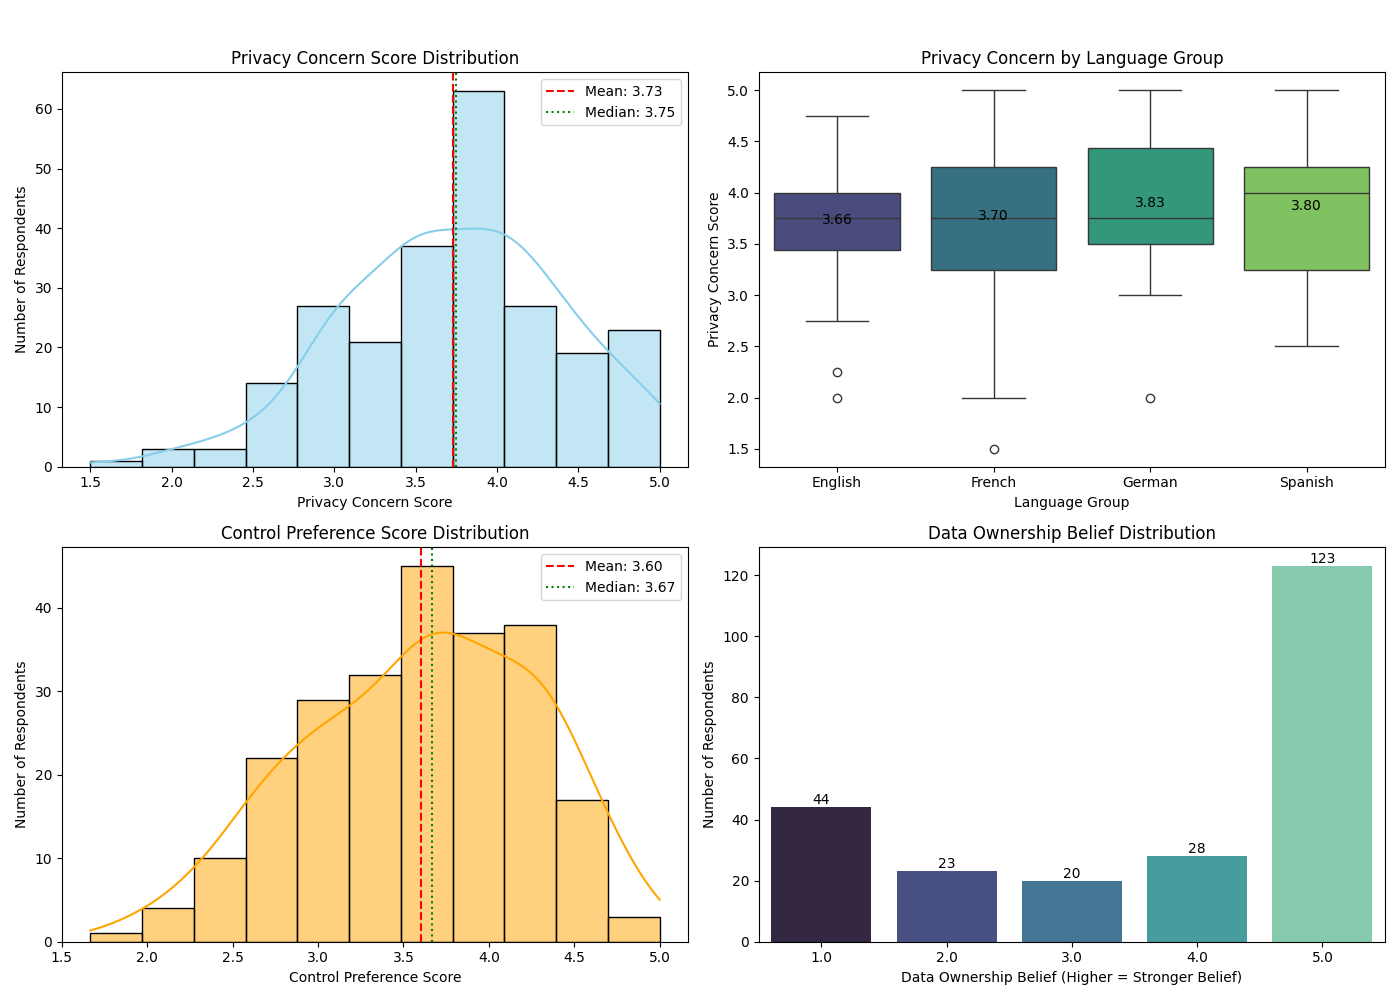
\includegraphics[width=\linewidth]{figures/img/derived_features_summary.png}
		\caption{Summary of Key Analytical Features}
		\label{fig:derived_features_summary}
	\end{figure}
	
	Another related feature, control preference, shows a distribution that is quite neutral but slightly positive towards desiring more control with a mean of 3.6/5 and a median of 3.67/5.
	Data ownership belief is however heavily skewed toward high belief in user ownership. Indeed, more than sixty percent of respondents believe in data ownership.     

	These features, will later be useful in order to make further analysis.
	\subsubsection{Segmentation}
This subsubsection presents the results of a cluster analysis designed to segment the sample into distinct user profiles. The aim here is to provide a structured, data-driven account of the diversity within the sample, highlighting how combinations of privacy concern, control preference, trust in technology, and data ownership belief can merge into interpretable attitudinal types.
The K-means clustering algorithm analysis revealed two distinct attitudinal profiles that were clear. \textit{Pragmatic Sharers}, and \textit{Skeptics} emerged as the two groups, each showing distinct engagement with technology, view privacy, and demographic.

\paragraph{Cluster 1: Pragmatic Sharers (n=179)} This cluster represents a younger demographic that is characterized by an active engagement with technology. A clear majority (65.9\%) are active users of connected health devices, and their demographic profile is dominated by the 25--34 age group (69.3\%) and students (35.2\%). French (65.4\%) and English (21.8\%) speakers dominate this group, with a generally higher level of education.

Attitudinally, this group is defined by a high willingness to share data (81.6\%) paired with the strongest preference for control over that data (mean score of 3.69/5). While their trust in technology is moderate (3.16), it is higher than the other cluster. Their privacy concern remains high (3.66), nearly matching the Skeptics group, indicating that their willingness to share is not due to a lack of concern.

\paragraph{Cluster 2: Skeptics (n=59)} In an interesting contrast, this smaller cluster embodies a more cautious and distrustful stance. A significant majority (67.8\%) are non-users of connected health devices. Demographically, they represent an older group, with members concentrated in the 45--54 (30.5\%) and 55--64 (42.4\%) age brackets, and are predominantly Spanish (45.8\%) or German (35.6\%) speakers.

Their scores highlight their skepticism, with the highest privacy concern (3.9/5) and the lowest trust in technology (2.56/5) This makes them the least willing to share data, with only 47.5\% of members open to it. Their moderate desire for control (3.35) and strong belief in user data ownership (3.97) reinforce their cautious mindset.

\begin{table*}[ht] 
	\caption{Summary of Key Cluster Results}
	\centering
	\begin{tabular}{lcc}
		\toprule
		& \textbf{Cluster 0: Skeptics} & \textbf{Cluster 1: Pragmatic Sharers} \\
		\midrule
		Size & 59 & 179 \\
		Privacy Concern Score & 3.94 (highest) & 3.66 \\
		Control Preference Score & 3.35 & 3.69 (highest) \\
		Tech Trust Score & 2.56 (lowest) & 3.16 \\
		Data Ownership Belief & 3.97 & 3.59 \\
		Willingness to Share & 47\% (lowest) & 82\% (highest) \\
		Main Age Groups & 45--64 (73\%) & 25--34 (69\%) \\
		User Type & 68\% Non-users & 66\% Users \\
		Dominant Language & Spanish/German & French/English \\
		Occupation & Employed/Retired/Self-employed & Student/Employed \\
		\midrule
		Stance & \parbox{6cm}{Highest privacy concern, lowest trust in technology, lowest willingness to share. Predominantly older, non-users.} & \parbox{6cm}{High willingness to share, strong control preference, moderate trust. Mainly younger, active users.} \\
		\bottomrule
	\end{tabular}
	\label{tab:cluster_summary_brief}
\end{table*}
	\subsubsection{Qualitative Insights}
		% Open-ended responses, word cloud, main themes
		Response to Q21 complement the quantitative data by highlighting participants' experiences and priorities. Participants often used straightforward language, highlighting distrust in centralized data handlers and a strong push for user agency. The language used is often direct and unambiguous, reflecting a persistent skepticism toward centralized data handlers and a pronounced desire for greater user agency.
		The world cloud (\autoref{fig:q21_wordcloud}) reveals frequently used terms, like 'protect people' as the most prominent term, alongside others like 'business', 'power', and 'difficult'. Several respondents explicitly referenced a lack of trust in corporations, using phrases such as “companies always find a way to exploit data” and “I don’t believe my data is safe, no matter what they promise.” Others emphasized the importance of user control, with comments like “I want to decide who sees my health data, not just accept terms” and “full control should be the default, not the exception.”
		
		\begin{figure}[h!]\centering
			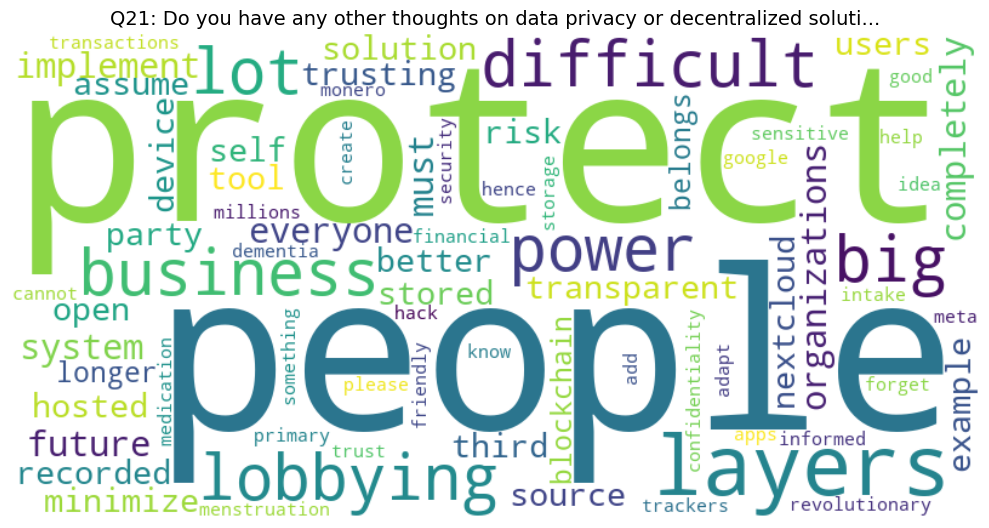
\includegraphics[width=1\linewidth]{figures/questions/Q21_wordcloud.png}
			\caption{Word Cloud of Open-Ended Responses on Data Privacy and Decentralized Solutions (Q21)}
			\label{fig:q21_wordcloud}
		\end{figure}

		Recurring themes frequently expressed frustration with current privacy measures and called for simpler, more transparent data management tools. Several participants shared their frustration about the lack of transparency in current systems, particularly around who has access to their data and why. The demand for transparency, seen in calls for 'clear rules' and 'easy-to-understand privacy setting', pointing to a mismatch between what user expects and reality. 
		Some responses highlighted interest in open-source and self-hosted solutions, seeking more control over their data. Though some comments showed frustration with the pace of changing privacy policies, there was no real sign of apathy. Rather, participants showed cautious engagement, with a clear desire for real control over their data instead of passive acceptance.
		Table~\ref{tab:qualitative_themes} summarizes the main themes and representative quotes.

		\begin{table*}[ht]
			\caption{Main Themes from Open-Ended Responses (Q21)}
			\centering
			\begin{tabular}{p{3.5cm}p{11cm}}
				\toprule
				\textbf{Theme} & \textbf{Representative Quotes} \\
				\midrule
				Skepticism toward Centralization & “Companies always find a way to exploit data.”; “I don’t believe my data is safe, no matter what they promise.” \\
				Demand for User Control & “I want to decide who sees my health data, not just accept terms.”; “Full control should be the default, not the exception.” \\
				Transparency & “Clear rules are needed.”; “I want to know who accesses my data.”; “Privacy settings should be easy to understand.” \\
				Open-Source/Self-Hosted & “I would trust an open-source platform more than a big tech company.”; “Self-hosted data vaults are the only way to be sure.” \\
				Privacy Fatigue & “It’s impossible to keep up with all the changes.”; “I just accept the risks because I want the benefits.” \\
				\bottomrule
			\end{tabular}
			\label{tab:qualitative_themes}
		\end{table*}
\subsection{Axis 1: Ethical Responsibilities and Deontological Perspectives}
	\subsubsection{Privacy Concern}
		% Distribution and levels of privacy concern (Q4, composite score)
		% Subgroup differences (user type, language, age)
		Privacy concern is a significant and widespread sentiment within the sample. When asked directly about their concern for health data privacy (Q4), respondents showed a right-skewed distribution with a mean of 3.45 out of 5, indicating a moderate to high level of concern, as seen in Figure~\ref{fig:privacy_concern_q4}. Over half of the participants (52\%) reported high or very high concern, while a quarter (25\%) expressed low or no concern. A notable 23\% selected the neutral option, suggesting a significant degree of ambivalence.
		Correlation analysis confirms that privacy concern is strongly associated with several key attitudinal and demographic variables. The positive correlations are with the \textit{Skeptics} cluster ($r = 0.28$, $p < 0.001$) and control preference score ($r = 0.23$, $p < 0.001$). Conversely, concern is negatively correlated with the \textit{Pragmatic Sharers} cluster ($r = -0.28$, $p < 0.001$).
		Demographics play a clear role. Age is a significant factor, with concern increasing with age. The oldest groups (65+ and 55--64) show significant positive correlations ($r = 0.22$ and $r = 0.18$, respectively), while the youngest groups show significant negative correlations. Occupation mirrors this trend, with students exhibiting a strong negative correlation ($r = -0.26$, $p < 0.001$) and retired individuals a positive one ($r = 0.16$, $p < 0.05$). Language group is also a differentiator: Spanish speakers are positively correlated with higher concern ($r = 0.21$, $p < 0.001$), while French speakers are negatively correlated ($r = -0.19$, $p < 0.01$).
		Subgroup analysis further details these patterns. Non-users report slightly higher levels of 'very high' concern (27.7\%) compared to users (21.2\%). An inverse relationship is observed with tech trust; as trust in technology increases, expressed privacy concern tends to decrease. However, no clear pattern emerges when comparing privacy concern with data ownership belief.
		\begin{figure}[h!]\centering
			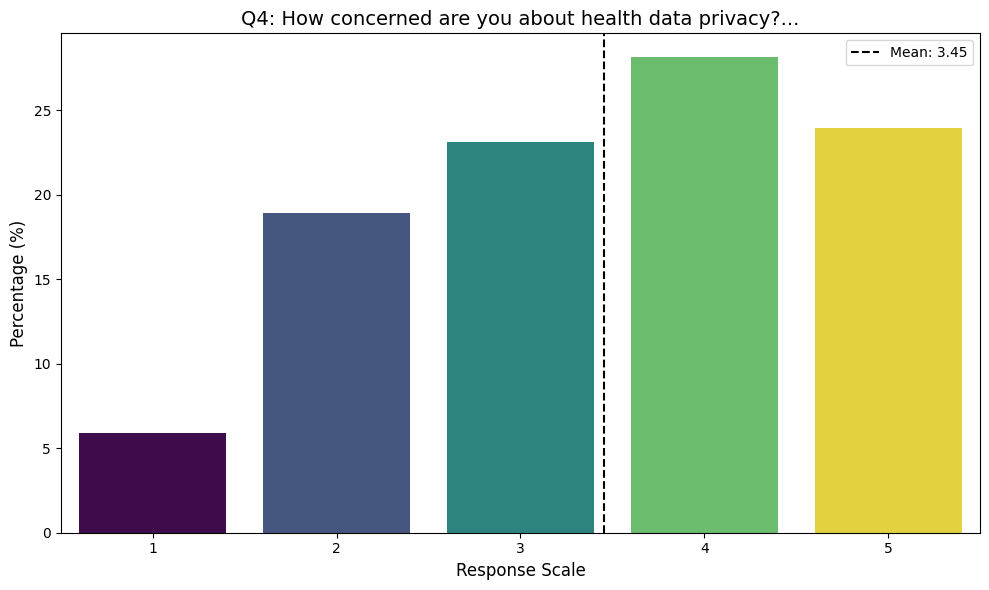
\includegraphics[width=1\linewidth]{figures/questions/Q4_likert.png}
			\caption{Distribution of Privacy Concern (Q4: 'I am concerned about the privacy of my wearable data')}
			\label{fig:privacy_concern_q4}
		\end{figure}
	\subsubsection{Trust}
		% Trust in companies (Q1), comparison with external benchmarks
		As the literature showed, trust is critical for the adoption of decentralized data management technologies. In this sample, trust was assessed using a single Likert-scale item (Q1: “How much do you trust current centralized systems (where companies store and manage your data) to protect your health information?”), showing a distribution centered at the neutral midpoint (mean = 2.67). Only a small fraction of respondents (~30\%) expressed “Complete trust,” while (40\%) indicated “Low” or “No trust.” The majority of responses clustered around neutrality, as visualized in Figure~\ref{fig:trust_q1}, with a slight right skew towards lower trust levels. 
		\begin{figure}[h!]\centering
			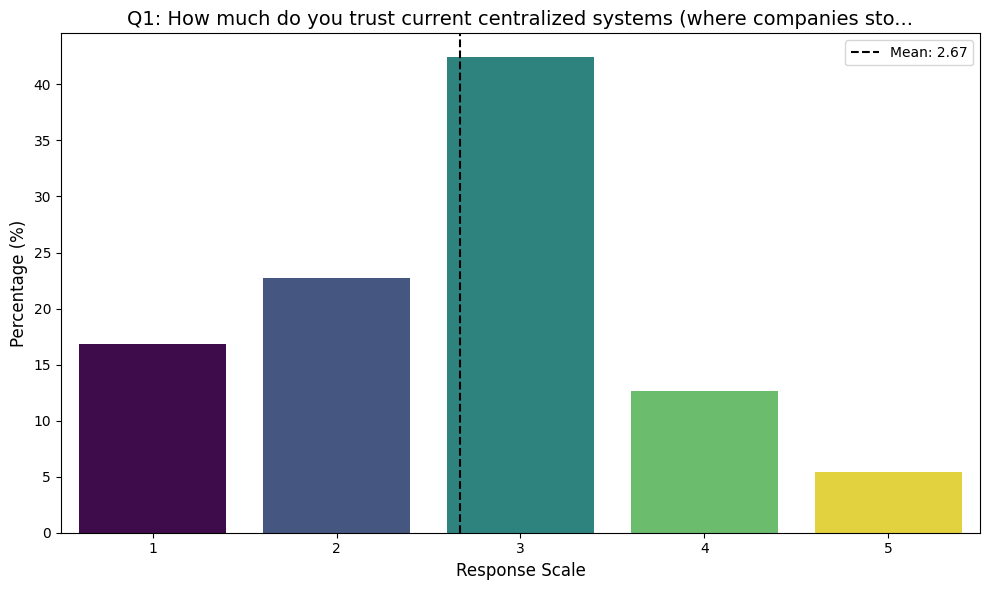
\includegraphics[width=1\linewidth]{figures/questions/Q1_likert.png}
			\caption{Distribution of Trust in Centralized Data Handlers (Q1: 'I trust companies to handle my wearable data responsibly')}
			\label{fig:trust_q1}
		\end{figure}
		Correlation analysis reveals that trust in centralized systems is significantly associated with only three variables. The strongest relationship is a very strong negative correlation with privacy concern score ($r = -0.74$, $p < 0.001$). There is also a strong positive correlation with general tech trust score ($r = 0.46$, $p < 0.001$). Age shows a weak but significant negative correlation, with the 65+ age group being less trusting ($r = -0.15$, $p < 0.05$).
		Subgroup analyses reinforce these patterns. Trust levels decrease as privacy concern or control preference scores increase. Conversely, trust in centralized handlers increases with general trust in technology. Most demographic variables show minimal divergence, but age stratification confirms a modest trend where trust decreases in older age groups. The \textit{Pragmatic Sharers} cluster exhibits a weak positive correlation with trust, while the \textit{Skeptics} show a weak negative correlation.

		\paragraph{Regression}
		A linear regression model was estimated to identify the primary drivers of trust in new decentralized technologies (Q13). The model accounts for approximately 29.2\% of the variance in trust ($R^2 = 0.292$), indicating low-moderate explanatory power. Attitudinal factors are the most significant predictors.
		Two variables stand out with strong and statistically significant effects, but in opposite directions. The \textit{privacy concern score} is a strong negative predictor ($\beta = -0.61$, $p < 0.001$), meaning that higher privacy concern is associated with lower trust in new technologies. In contrast, the \textit{control preference score} is a strong positive predictor ($\beta = 0.59$, $p < 0.001$), showing that a greater desire for personal control over data corresponds to higher trust in decentralized solutions.
		Other variables in the model---belief in data ownership, age, and education level---did not show statistically significant effects on trust in new technologies.

		\paragraph{Trust in Data Handlers: Survey vs. Pew}
		A comparative look at trust in data handlers, using both the thesis survey and the 2023 Pew Research Center dataset, provides a useful external anchor for situating the empirical findings within a broader context. Both instruments probe the degree of trust individuals place in organizations responsible for managing their personal data, albeit with different reference points and response scales. In the thesis survey, respondents were asked to rate their trust in current centralized systems—where companies store and manage health information—on a five-point Likert scale. The Pew item, while focused on social media company leaders and their willingness to admit mistakes and take responsibility for data misuse, offers a parallel perspective on institutional trustworthiness in the digital domain.
		
		Figure~\ref{fig:trust_q1} visualizes the distribution of trust responses in the thesis sample. The pattern is centered at the neutral midpoint: 42.4\% of respondents selected “3,” indicating neither trust nor distrust. At the upper end, only 5.5\% expressed the highest level of trust (“5”), and 12.6\% chose “4,” together accounting for less than one-fifth of the sample. On the lower end, 22.7\% selected “2” and 16.8\% chose “1,” yielding a combined 39.5\% who report low or no trust in centralized data handlers. The overall distribution is thus marked by a concentration at neutrality, with a slight tilt toward skepticism.
		
		\begin{figure}[h!]\centering
			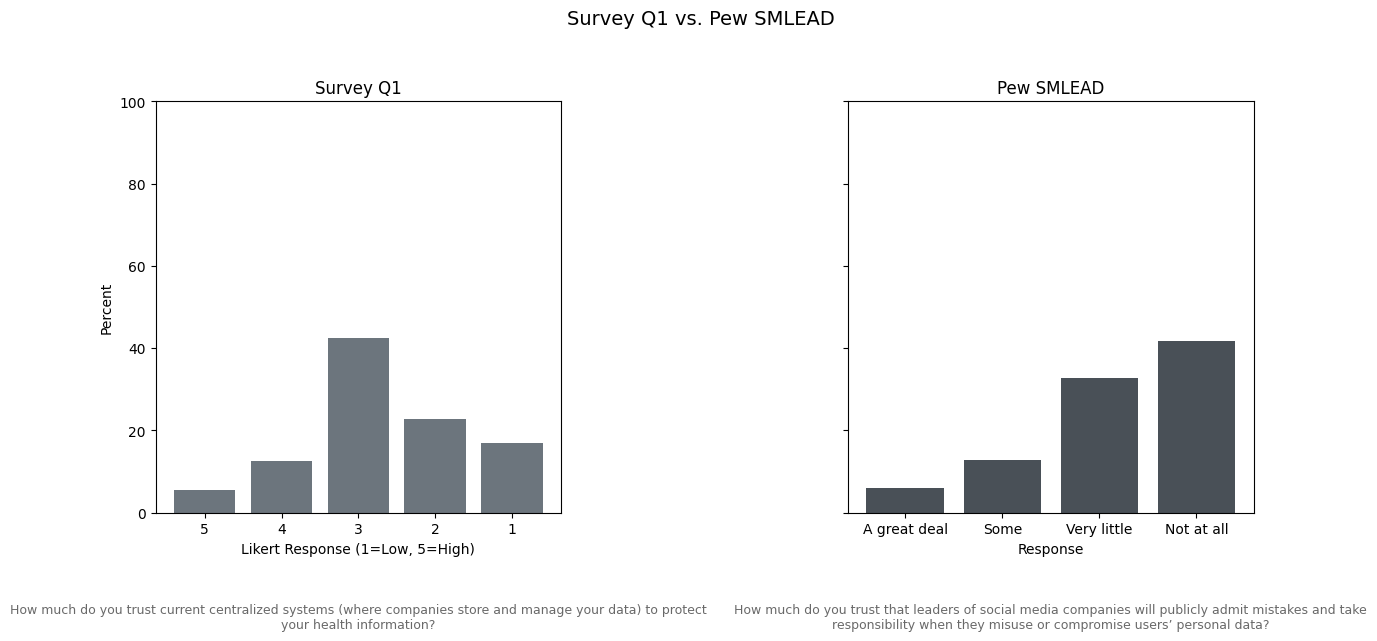
\includegraphics[width=1\linewidth]{figures/img/Pew_comparison_plots/compare_1_vs_SMLEAD.png}
			\caption{Trust in Centralized Data Handlers: Survey vs. Pew Research Center (2023)}
			\label{fig:trust_Pew_comparison}
		\end{figure}
		Turning to the Pew benchmark, the distribution is compressed into four categories and framed around trust in social media company leaders to admit mistakes and take responsibility for data misuse. Here, only 6\% of respondents report “A great deal” of trust, and 12.7\% indicate “Some” trust. The majority of responses are clustered at the lower end: 32.7\% select “Very little,” and 41.7\% choose “Not at all.” The Pew data thus reveal a pronounced deficit of trust, with nearly three-quarters of respondents expressing little or no confidence in the ethical conduct of data handlers.
		
		Direct comparison between the two samples requires some caution, given the differences in item wording, scale granularity, and the specific institutional focus. Nonetheless, several points of convergence and divergence are apparent. Both datasets reveal a scarcity of high-trust responses: only a small minority in each sample express strong confidence in the organizations managing their data. The Pew sample, however, displays a sharper polarization, with a larger share concentrated in the lowest trust category (“Not at all”) and a smaller proportion at the midpoint. In contrast, the thesis sample is characterized by a modal response at neutrality, with fewer respondents gravitating to the extremes.
		
		The central tendency in both datasets is clear: trust in data handlers—whether conceptualized as companies managing health information or as social media leaders—is limited. High trust is rare, and the prevailing sentiment is one of ambivalence or skepticism. The thesis sample’s distribution, with its pronounced midpoint, suggests a degree of uncertainty or withholding of judgment, whereas the Pew data reflect a more decisive lack of confidence.
		
		Subgroup analysis within the thesis sample, as detailed in earlier sections, indicates that trust in centralized data handlers is stable across user types, language groups, and age brackets. No substantial differences emerge by education or device usage frequency. The Pew dataset, while not segmented identically for this comparison, similarly points to a broad-based skepticism that cuts across demographic lines.
		
		Figure~\ref{fig:trust_Pew_comparison} overlays the two distributions, highlighting both the shared scarcity of high-trust responses and the differing patterns of polarization and neutrality. The juxtaposition of these results underscores the empirical regularity of limited trust in institutional data handlers, regardless of the specific context or framing.
		
		In summary, the external benchmarking exercise situates the thesis findings within a wider empirical landscape. Both the thesis and Pew samples reveal that strong trust in organizations responsible for managing personal data is the exception rather than the rule. The thesis sample’s tendency toward neutrality contrasts with the Pew sample’s sharper tilt toward distrust, but the overarching message is consistent: confidence in data handlers remains fragile, and high trust is in short supply. These patterns provide a quantitative anchor for the subsequent analysis of privacy concern, control, and openness to alternative data management paradigms.
	\subsubsection{Responsibility}
		% Who is responsible? (Q19)
		The question of who should bear primary responsibility for the ethical use of wearable health data reveals a divided but structured set of opinions. As shown in Figure~\ref{fig:responsibility_q19}, there is no single consensus. 'Shared responsibility' was the most frequent choice (34.0\%), followed by 'Device manufacturers/companies' (27.7\%), 'Individual users' (20.2\%), and 'Government regulators' (17.2\%).
		\begin{figure}[ht]\centering
			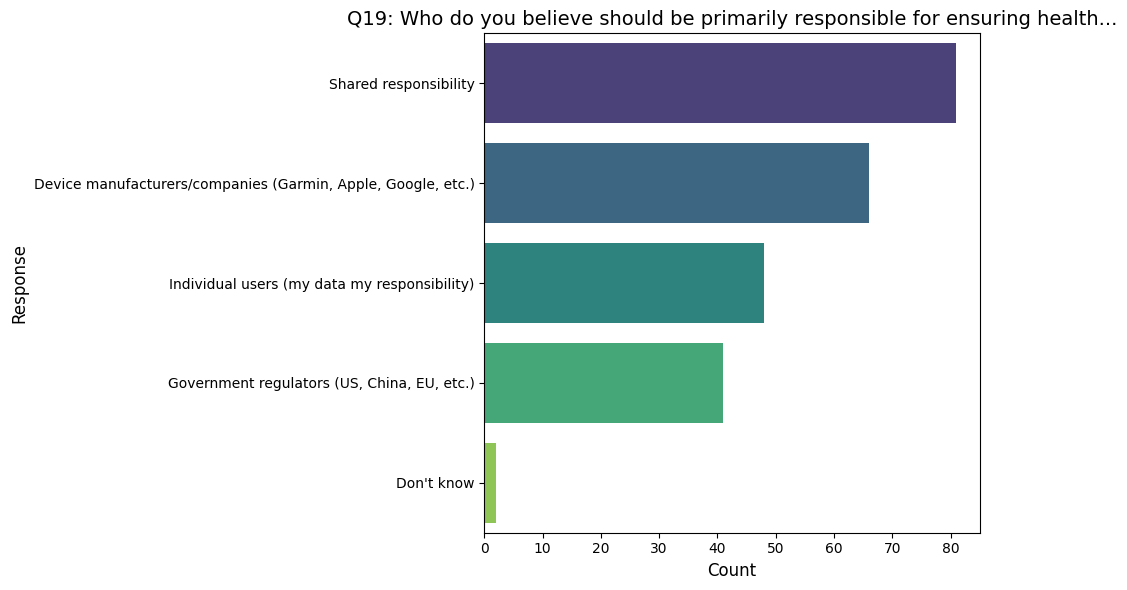
\includegraphics[width=1.0\textwidth, height=0.55\textheight, keepaspectratio]{figures/img/subgroup_ana/Q19_overall_dist.png}
			\caption{Distribution of Responsibility Attribution (Q19: 'Who should be primarily responsible for the ethical use of wearable health data?')}
			\label{fig:responsibility_q19}
		\end{figure}
		Correlation analysis and subgroup distributions indicate that these attributions of responsibility are not random, but are linked to attitudinal and demographic profiles established throughout this study. The most pronounced effects are observed across user clusters. Placing responsibility on the 'Individual User' is strongly and positively correlated with the \textit{Skeptics} cluster ($r = 0.32$, $p < 0.001$), with 50.9\% of this group selecting this option. Conversely, this choice is negatively correlated with the \textit{Pragmatic Sharers} cluster ($r = -0.32$, $p < 0.001$). The opposite pattern holds for attributing responsibility to 'Device Manufacturers,' which is positively correlated with the \textit{Pragmatic Sharers} ($r = 0.14$, $p < 0.05$) and negatively with the \textit{Skeptics} ($r = -0.14$, $p < 0.05$).
		This division is mirrored in user typology. Device users are significantly more likely to hold companies responsible (35.8\% vs. 16.8\% for non-users) and less likely to choose individual responsibility (14.6\% vs. 27.7\%). This aligns with correlations showing 'user\_type\_User' is positively correlated with blaming manufacturers ($r = 0.21$, $p < 0.01$) and negatively with blaming individuals ($r = -0.16$, $p < 0.05$).
		Cultural and demographic factors are also significant. German speakers show a positive correlation with selecting 'Individual Users' ($r = 0.27$, $p < 0.001$), with 54.5\% of them choosing this option, a stark contrast to other language groups. Age also shows a clear trend: the 65+ group is correlated with selecting individual responsibility ($r = 0.28$, $p < 0.001$), while the 18--24 group is negatively correlated with this choice ($r = -0.18$, $p < 0.01$) and positively correlated with holding manufacturers responsible ($r = 0.20$, $p < 0.01$).
		Attitudinal variables show weaker but consistent patterns. Higher privacy concern is weakly correlated with assigning responsibility to individuals ($r = 0.16$, $p < 0.05$). Lower trust in technology ($r = -0.17$, $p < 0.01$) and a lower preference for control ($r = -0.17$, $p < 0.05$) are also associated with choosing individual responsibility.
\subsection{Axis 2: Digital Sovereignty and Consumer Empowerment}
	\subsubsection{Perceived Control Over Data}
		% Perceived control (Q2), desired control (Q3), gap analysis
		A sense of disempowerment characterizes respondents' relationship with their wearable data. When asked to rate their perceived level of control (Q2), a clear majority (65\%) reported having 'No control' or 'Low control,' with a mean score of only 2.28 out of 5. Conversely, a mere 12.2\% felt they had 'High' or 'Complete' control, as illustrated in Figure~\ref{fig:perceived_control_q2}.
		\begin{figure}
			\centering
			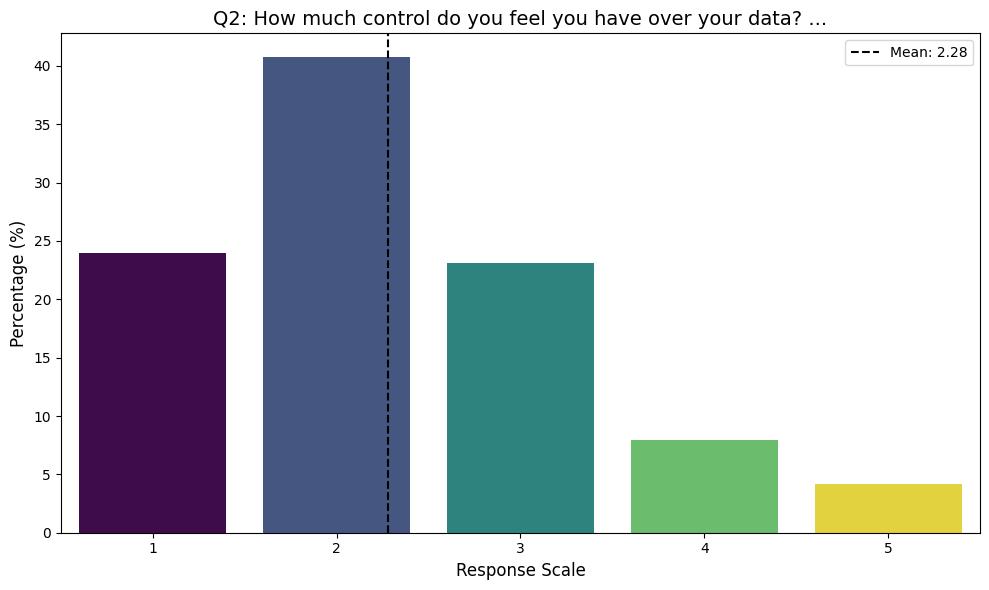
\includegraphics[width=1\linewidth]{figures/questions/Q2_likert.png}
			\caption{Distribution of Perceived Control Over Wearable Health Data (Q2)}
			\label{fig:perceived_control_q2}
		\end{figure}
		Correlation analysis reveals that this perception of control is not arbitrary but is linked to underlying attitudes. The most significant factor is \textit{privacy concern score}, which has a strong negative correlation with perceived control ($r = -0.62$, $p < 0.001$). This inverse relationship is starkly visible in the subgroup distributions: among respondents with 'Very High' privacy concern, 55.1\% report having 'No control,' whereas no respondents in the 'Low' concern group report this, and 50\% of them feel they have 'Complete control.'
		Conversely, a higher \textit{tech trust score} is positively correlated with a greater sense of control ($r = 0.19$, $p < 0.01$). Language group also emerges as a differentiator, with Spanish speakers feeling more in control ($r = 0.20$, $p < 0.01$) and French speakers feeling less so ($r = -0.17$, $p < 0.01$). Notably, key variables such as user type, age, and cluster profile do not show statistically significant correlations with perceived control, although subgroup distributions suggest \textit{Skeptics} feel slightly less control than \textit{Pragmatic Sharers}.
	\subsubsection{Perceived Control: Survey vs. Pew}
		A comparative analysis of perceived control over personal data, drawing on both the thesis survey and the 2023 Pew Research Center dataset, offers a external reference point for situating the findings within a broader context. While the two instruments differ in their precise wording and response scales, both probe the extent to which individuals feel they can influence the fate of their personal information in digital environments. In the thesis survey, respondents were asked, “How much control do you feel you have over your data?” using a five-point Likert scale, whereas the Pew item focuses on “How much control do you think you have over the data that companies collect about you?” with a four-point scale. Despite these differences, the underlying construct, perceived agency in the management of personal data, remains closely aligned.
		Figure~\ref{fig:Pew_control_comparison} visualizes the distribution of responses in both samples. In the thesis dataset, as we have seen, the pattern is skewed toward the lower end of the control spectrum.			
		For Pew benchmark, the distribution is similarly weighted toward lower perceived control, though the scale is compressed. Only 4\% of Pew respondents report having “A great deal of control,” and 18\% indicate “Some control.” The majority of responses are concentrated in the “Very little control” (51\%) and “No control” (27\%) categories, yielding a combined 78\% who perceive themselves as largely powerless in the face of data collection by companies. The absence of a neutral midpoint in the Pew scale may contribute to the sharper polarization, but the overall pattern is consistent: high perceived control is rare, and the prevailing sentiment is one of limited agency.
		Direct comparison between the two samples requires some caution, given the differences in item phrasing and response options. Nonetheless, several points of convergence are evident. Both datasets reveal a pronounced skew toward low perceived control, with only a small minority expressing confidence in their ability to manage or influence the use of their personal data. The thesis sample, with its focus on wearable health data, displays a slightly higher proportion in the lowest category (“1”) compared to the Pew sample’s “No control,” but the overall shape of the distributions is remarkably similar. The central tendency in both cases is clear: most individuals do not feel in command of their digital footprints, whether in the context of health data or more general data collection by companies.
		In sum, the external benchmarking confirms that the observed deficit in perceived control is not unique to wearable health data users, but reflects a broader societal baseline. 		
	\begin{figure}[ht]\centering
		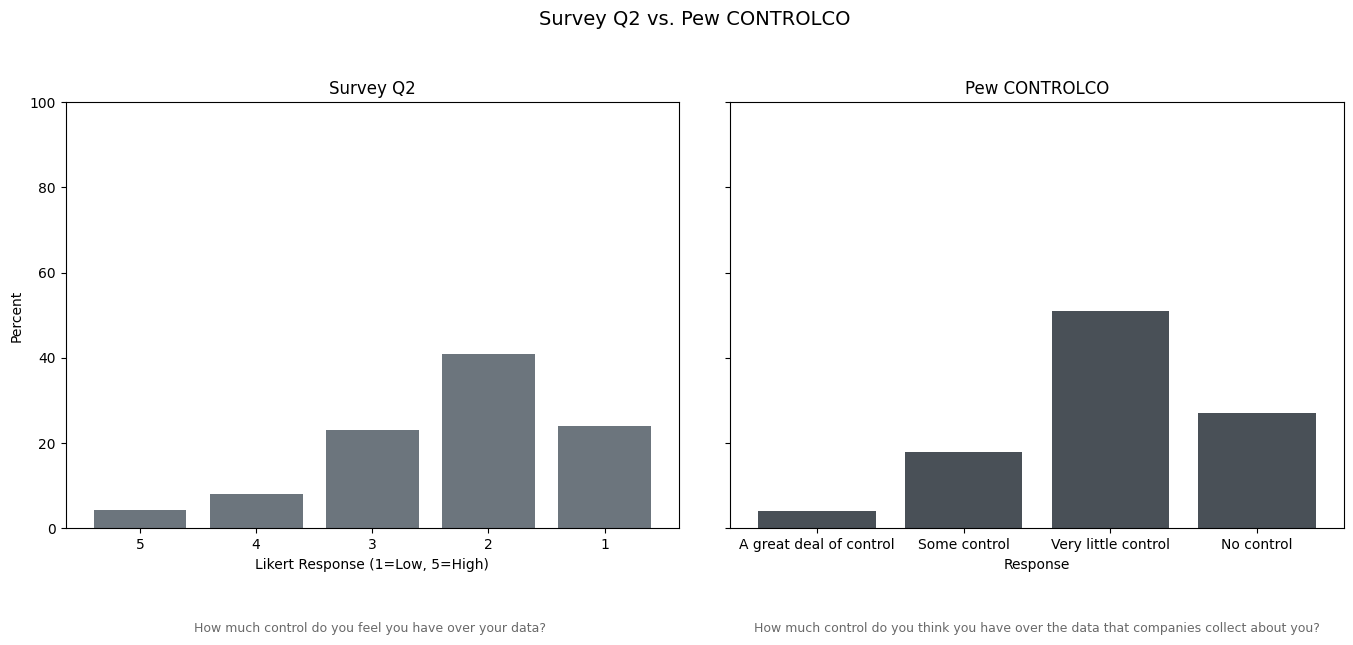
\includegraphics[width=1\linewidth]{figures/img/Pew_comparison_plots/compare_2_vs_CONTROLCO.png}
		\caption{Perceived Control Over Personal Data: Thesis Sample vs. Pew Research Center (2023)}
		\label{fig:Pew_control_comparison}
	\end{figure}
	\subsubsection{Desired Control Over Data}
		% Desired control (Q3), distribution and subgroup differences
		In stark contrast to their perceived lack of control, respondents expressed an overwhelming and strong desire for greater agency over their data. When asked to rate their desired level of control (Q3), 85\% of respondents selected 'High' or 'Complete' control, resulting in a strongly left-skewed distribution with a mean score of 4.41 out of 5 (Figure~\ref{fig:desired_control_q3}). 
		\begin{figure}[ht]\centering
			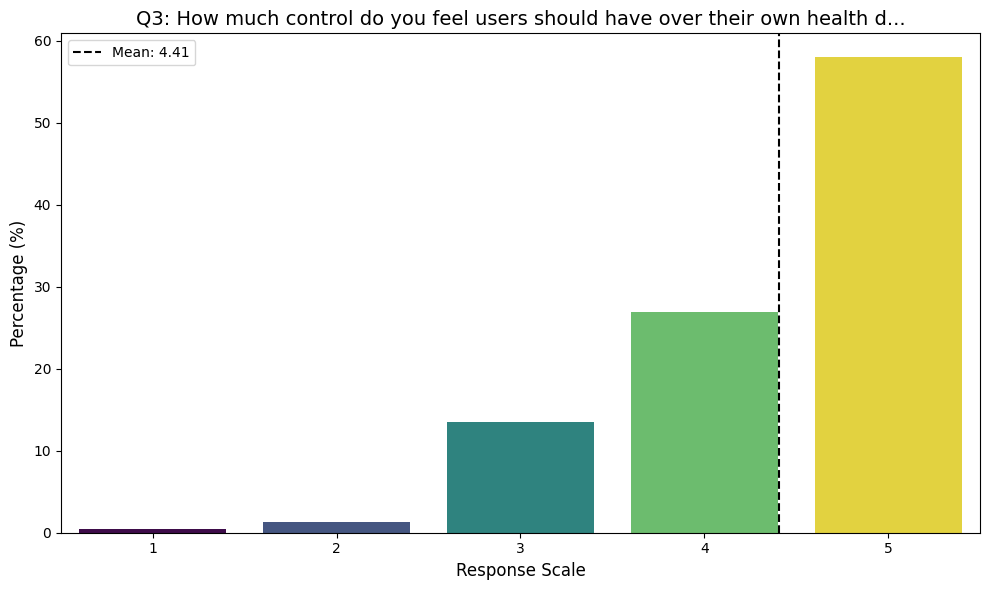
\includegraphics[width=1\linewidth]{figures/questions/Q3_likert.png}
			\caption{Distribution of Desired Control Over Wearable Health Data (Q3)}
			\label{fig:desired_control_q3}
		\end{figure}
		This sentiment is consistent across most demographic and behavioral subgroups, including user type, age, and education, where no statistically significant patterns emerged.
		The desire for control is not an isolated preference but is strongly linked to underlying privacy attitudes. Correlation analysis reveals a positive relationship between desired control and the privacy concern score ($r = 0.52$, $p < 0.001$). This trend is illustrated in the subgroup analysis: as privacy concern intensifies, the demand for complete control escalates, with 90\% of respondents in the 'Very High' concern category selecting 'Complete control,' compared to only 25\% in the 'Low' concern group. The control preference score, a composite variable of which this question is a part, shows a similarly strong positive correlation ($r = 0.46$, $p < 0.001$), confirming internal consistency. All other variables, including tech trust and data ownership belief, showed no statistically significant correlation with the desired level of control.
	\subsubsection{Belief in Data Ownership}
		% Data ownership belief (Q16), distribution and polarization	
		Respondents expressed a general belief that users should own the data generated by their wearable devices. When presented with this statement (Q16), a clear majority (60.2\%) either 'Strongly Agreed' (51.3\%) or 'Agreed' (9.2\%). In contrast, only 27.9\% disagreed, resulting in a distribution heavily skewed toward affirming user ownership (mean = 2.32, median = 1.00), as shown in Figure~\ref{fig:Q16_data_ownership}.
		\begin{figure}[ht]\centering
			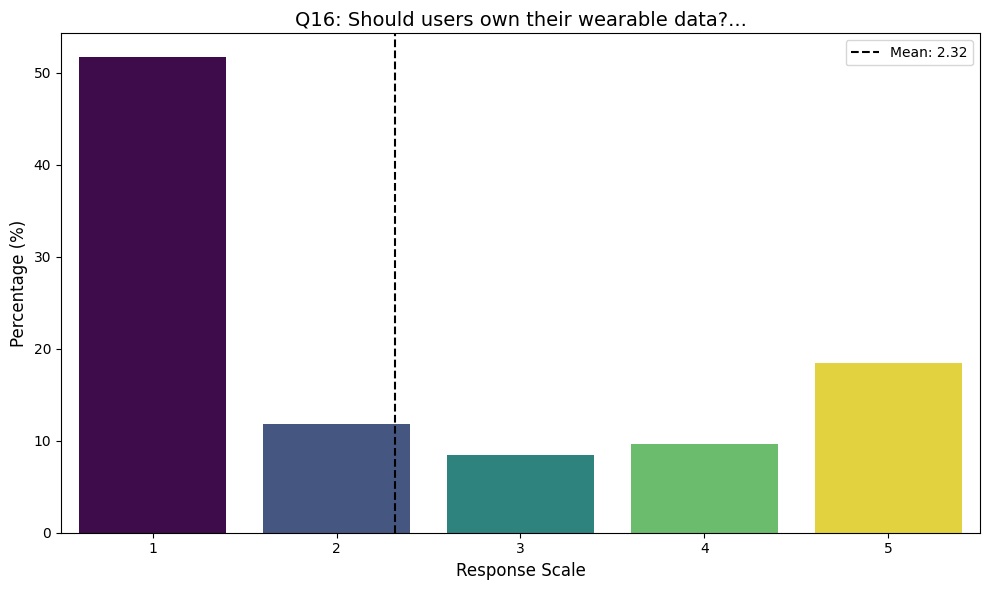
\includegraphics[width=1\linewidth]{figures/questions/Q16_likert.png}
			\caption{Distribution of Responses: 'Users should own the data generated by their wearable devices' (Q16)}
			\label{fig:Q16_data_ownership}
		\end{figure}
		A striking feature of this belief is its statistical independence from other core attitudes measured in this study. Correlation analysis reveals no significant relationship between the belief in data ownership and key variables such as privacy concern score, control preference score, or tech trust score. This independence is largely consistent across subgroups. While minor variations exist—for instance, the \textit{Skeptics} cluster shows slightly stronger agreement (61.0\%) than the \textit{Pragmatic Sharers} (48.6\%), these differences do not translate into significant correlations. The only statistically significant, but weak, correlation is with the 55--64 age group ($r = -0.13$, $p < 0.05$), indicating a slightly stronger agreement with user ownership within this demographic.
\subsection{Axis 3: Behavioral Science and User Decision-Making}
	\subsubsection{Willingness to Share Data}
		% Willingness to share for health insights (Q17), main barriers (Q18)
		Analysis of willingness to share wearable health data for health insights (Q17) shows that attitudes and behaviors matter much more than demographics. Most respondents (73.1\%) say they are willing to share, but this openness is linked to a few key predictors, as seen in Figure~\ref{fig:Q17_share}.
		\begin{figure}[ht]\centering
			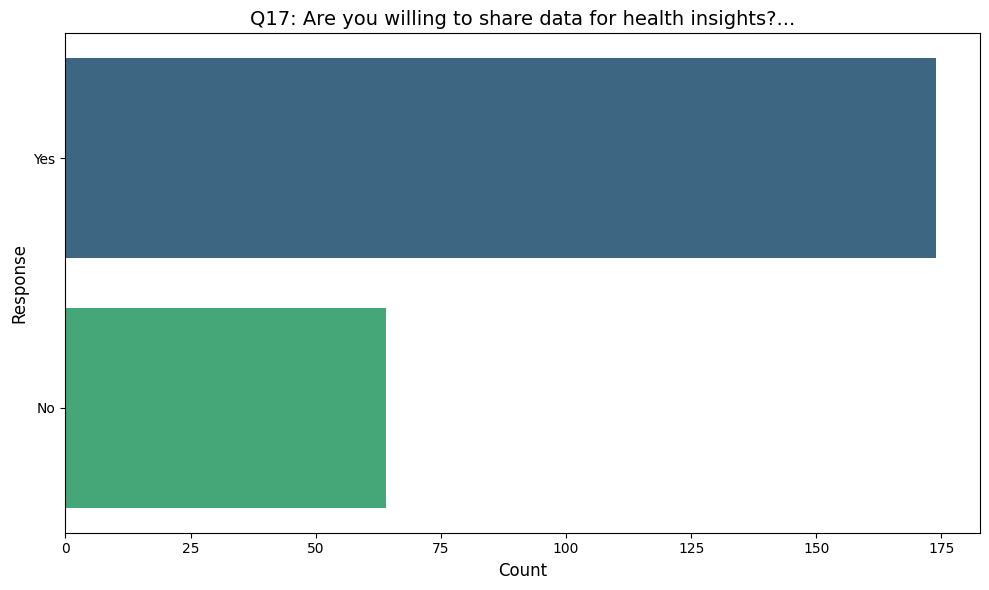
\includegraphics[width=1\linewidth]{figures/questions/Q17_single_choice.png}
			\caption{Willingness to Share Wearable Data for Health Insights (Q17)}
			\label{fig:Q17_share}
		\end{figure}
		Privacy concern is the main limiting factor, with a negative correlation to willingness to share ($r = -0.37$, $p < 0.001$). This is clear in subgroup results: among those with 'Moderate' concern, 93.2\% are willing to share, but this drops to just 50.7\% for those with 'Very High' concern.
		The  differences between the two main user clusters can alos be observed. \textit{Pragmatic Sharers} are much more likely to share ($r = +0.33$, $p < 0.001$), with 81.6\% agreeing. \textit{Skeptics} are the opposite ($r = -0.33$, $p < 0.001$), with only 47.5\% willing. This matches the user/non-user split: being a user is positively correlated ($r = +0.19$, $p < 0.01$), while being a non-user is negatively correlated ($r = -0.19$, $p < 0.01$).
		Tech trust also matters, though less strongly ($r = +0.20$, $p < 0.01$). Willingness to share rises from 47.6\% among those with the lowest trust to over 79\% for those with moderate or high trust.
		Demographics on the other hand play a smaller role. Younger respondents (18--24) are more likely to share ($r = +0.19$, $p < 0.01$), while older groups (45--54 and 65+) are less likely ($r = -0.17$ and $r = -0.18$, $p < 0.01$). Language group also matters: French speakers are more open ($r = +0.19$, $p < 0.01$), German speakers less so ($r = -0.26$, $p < 0.001$). Other factors—data ownership belief, control preference, education do not show significant effects.

		\paragraph{Barriers to Sharing}
		Among the 26.9\% of respondents unwilling to share their data, the cited barriers reveal a set of apprehensions. As shown in Figure~\ref{fig:Q18_barriers}, reluctance is primarily driven by fears of data 'Misuse' (70.5\%), 'Privacy loss' (68.9\%), a perceived 'No control' over data (63.9\%), and 'Breach risk' (52.5\%). The frequent selection of multiple barriers suggests these fears are deeply intertwined.
		\begin{figure}[ht]\centering
			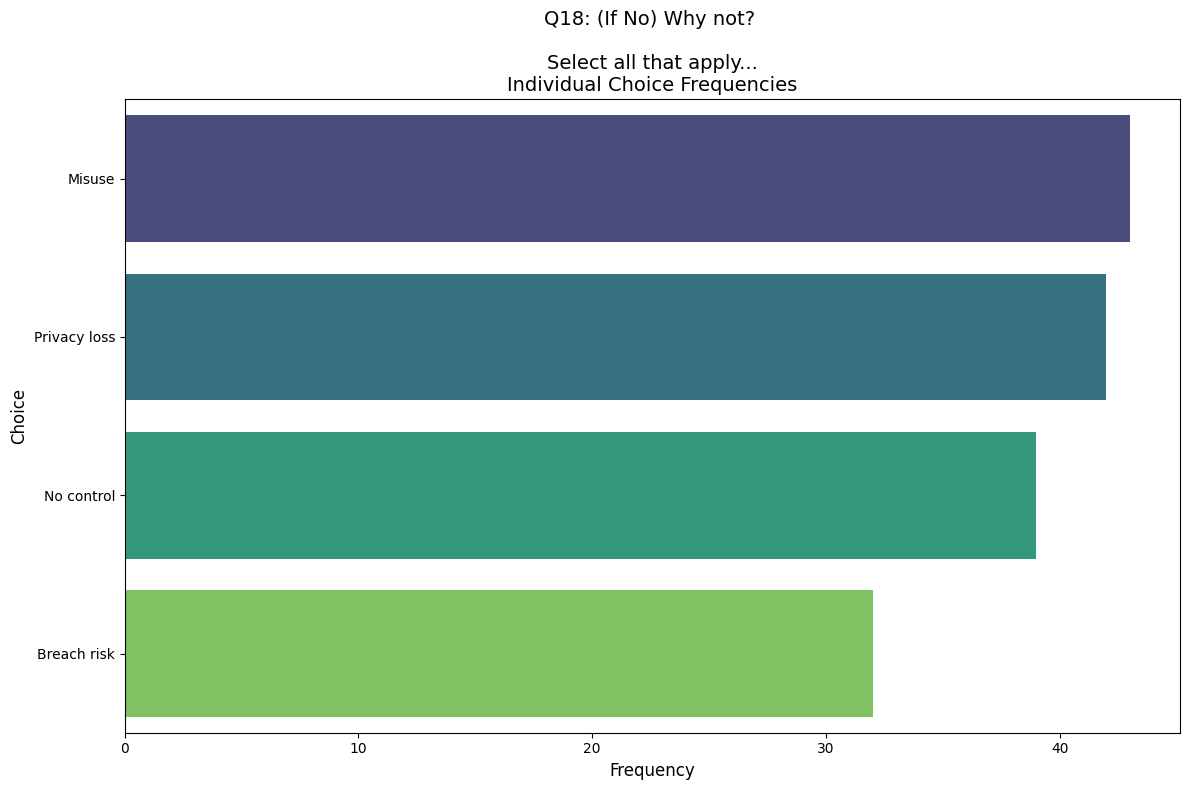
\includegraphics[width=1\linewidth]{figures/questions/Q18_multiple_choice.png}
			\caption{Main Barriers to Sharing Wearable Data (Q18, multiple responses allowed)}
			\label{fig:Q18_barriers}
		\end{figure}
		Correlation analysis confirms that these barriers are not uniform across the sample but are strongly related to specific attitudinal and demographic profiles. Privacy concern is the most significant correlate, showing a strong positive association with citing all four barriers, especially 'No control' ($r = 0.38$, $p < 0.001$) and 'Privacy loss' ($r = 0.34$, $p < 0.001$). Conversely, higher tech trust is moderately negatively correlated with citing 'No control' as a barrier ($r = -0.23$, $p < 0.001$).
		The two user clusters exhibit the most polarized patterns. The \textit{Skeptics} cluster is strongly and positively correlated with citing all major barriers (e.g., 'Privacy loss': $r = 0.30$, $p < 0.001$), whereas the \textit{Pragmatic Sharers} cluster shows an equally strong negative correlation (e.g., 'Privacy loss': $r = -0.30$, $p < 0.001$). This cleavage is mirrored in user typology, where non-users are significantly more likely to cite 'Misuse' ($r = 0.19$, $p < 0.01$) and 'Privacy loss' ($r = 0.18$, $p < 0.01$) as deterrents.
		Demographic factors also emerge as significant differentiators. Age is a consistent factor, with older groups (especially 65+) more likely to cite barriers like 'Privacy loss' ($r = 0.25$, $p < 0.001$), while the youngest group (18--24) is negatively correlated with citing all four. Language group is also a strong discriminant; German speakers show a robust positive correlation with citing all barriers (e.g., 'Misuse': $r = 0.30$, $p < 0.001$), while French speakers display a significant negative correlation, particularly with 'Privacy loss' ($r = -0.23$, $p < 0.001$).

		\paragraph{Regression}
		A logistic regression model was estimated to identify the primary predictors of willingness to share wearable health data for health-related insights (Q17). The model demonstrates weak explanatory power (Pseudo R² = 0.19) and reveals that attitudinal factors are the most significant drivers.
		Privacy concern emerges as the dominant negative predictor ($\beta = -1.60$, $p < 0.001$). The result is significant, and the negative coefficient indicates that as a respondent's privacy concern increases, their likelihood of being willing to share data decreases substantially.
		In contrast, other core attitudinal variables do not show a statistically significant effect in this model. Control preference ($\beta = 0.32$, $p = 0.25$), trust in technology ($\beta = 0.07$, $p = 0.73$), and data ownership belief ($\beta = 0.13$, $p = 0.22$) are not significant predictors of the willingness to share data once privacy concern is accounted for.
		Among demographic variables, education level is a modest but significant positive predictor ($\beta = 0.42$, $p = 0.03$), suggesting that individuals with higher educational attainment are more likely to be willing to share their data. Age shows a marginally significant negative trend ($\beta = -0.21$, $p = 0.09$), hinting that older respondents may be less willing to share.
	\subsubsection{Willingness to Adopt}
	% Q12
	Analysis of willingness to adopt decentralized data management solutions (Q12) indicates a generally positive inclination among respondents. The mean response is 3.71, with a median of 4.0 on a five-point scale. Most participants reported they would be "likely" (39.5\%) or "very likely" (26.9\%) to use such systems if they provided enhanced control over personal data, as seen in Figure~\ref{fig:Q12_willingness}.
	\begin{figure}[h!]\centering
		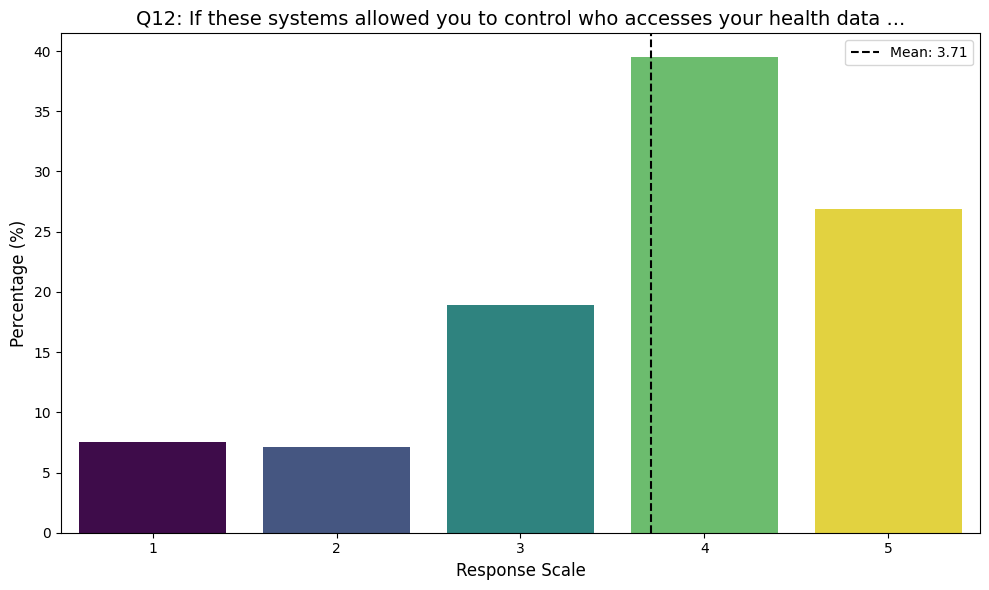
\includegraphics[width=1\linewidth]{figures/questions/Q12_likert.png}
		\caption{Willingness to Adopt Decentralized Data Management Solutions (Q12)}
		\label{fig:Q12_willingness}
	\end{figure}
	Correlation analysis highlights several strong predictors of this willingness. The most influential is the \textit{control preference score}, which demonstrates a strong positive correlation ($r = 0.77$, $p < 0.001$). Subgroup distributions confirm a monotonic relationship: willingness to adopt rises directly with preference for control, with all respondents at the highest control preference also expressing the highest willingness. Trust in new technologies (\textit{tech trust score}) is another positive predictor ($r = 0.41$, $p < 0.001$).
	User clusters show polarization. The \textit{Pragmatic Sharers} cluster is significantly and positively correlated with willingness to adopt ($r = 0.28$, $p < 0.001$), while the \textit{Skeptics} cluster is equally strongly negatively correlated ($r = -0.28$, $p < 0.001$). This pattern matches the finding that current device users are more willing to adopt ($r = 0.19$, $p < 0.01$) than non-users ($r = -0.19$, $p < 0.01$).
	Demographic factors reveal nuanced effects. Willingness is positively correlated with the 25--34 age group ($r = 0.20$, $p < 0.01$) and negatively with the 55--64 age group ($r = -0.17$, $p < 0.01$). Education shows a divergent pattern: holding a Master's degree is positively correlated with willingness ($r = 0.19$, $p < 0.01$), while holding a Doctorate (PhD) is negatively correlated ($r = -0.17$, $p < 0.05$). Subgroup data confirms that 40\% of respondents with a PhD are "not at all" interested.
	The relationship with privacy concern is non-linear and does not show a significant linear correlation. Subgroup analysis, however, reveals polarization among those with the highest privacy concern: they are both the most likely to be "very likely" to adopt (36.2\%) and have a notable share who are "not at all" interested (15.9\%).

	\paragraph{Regression}
	An ordinal regression model was build to identify the key predictors of willingness to adopt decentralized data management solutions (Q12),	with feature leakage corrected. The results indicate that attitudinal factors are the primary drivers of adoption intention.
	The strongest predictor is the clean control preference score (\texttt{control\_preference}), which exerts a highly significant positive effect on willingness to adopt ($\beta = 0.84$, $p < 0.001$). This suggests that a greater preference for personal control over data is strongly associated with increased interest in decentralized systems. Trust in new technologies (\texttt{tech\_trust\_score}) is also a significant positive predictor ($\beta = 0.66$, $p < 0.001$), indicating that higher trust correlates with greater willingness to adopt.
	Other variables, including privacy concern score ($\beta = -0.11$, $p = 0.636$), data ownership belief ($\beta = -0.03$, $p = 0.664$), age, and education level, do not show statistically significant effects. These findings suggest that adoption decisions are shaped more by proactive control preferences and trust in new solutions than by general privacy anxiety or demographic profile.
	\subsubsection{Privacy Policy Engagement}
	% Reading/skimming privacy policies (Q10), external benchmark
	Engagement with privacy policies among wearable device users is characterized by widespread disengagement. The data reveal a clear pattern of avoidance: a majority of users (67.6\%) report not reading policies at all, while 25.7\% indicate they only skim them. A small minority (6.6\%) claims to read them fully, as shown in Figure~\ref{fig:Q10_policy_engagement}.
	\begin{figure}[ht]\centering
		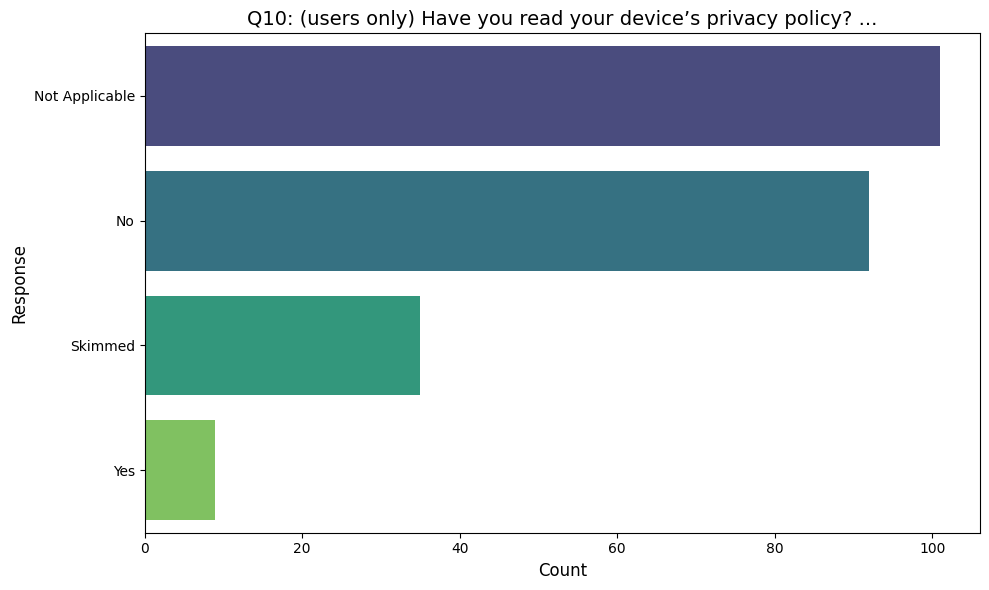
\includegraphics[width=1\linewidth]{figures/questions/Q10_single_choice.png}
		\caption{Privacy Policy Engagement: Reading vs. Skimming (Q10)}
		\label{fig:Q10_policy_engagement}
	\end{figure}
	This behavior, however, is not uniform as correlation analysis shows it is associated with specific attitudinal and demographic profiles. A user's level of privacy concern is a key differentiator, showing a significant negative correlation with not reading policies ($r = -0.19$, $p < 0.01$). This indicates that individuals with higher concern are more likely to engage with policy documents. The effect is pronounced in subgroup analysis: 75\% of users with 'Low' concern ignore policies, a figure that drops to 33.3\% for those with 'Very High' concern.
	The user clusters also exhibit a significant relationship. The `Pragmatic Sharers' cluster is positively correlated with not reading policies ($r = 0.24$, $p < 0.001$), a finding that aligns with their more utilitarian approach to data sharing.
	Age emerges as another factor. The youngest group (18--24) is more likely to ignore policies ($r = 0.14$, $p < 0.05$), whereas the oldest (65+) is less likely to do so ($r = -0.16$, $p < 0.05$) and, conversely, more likely to read them in full ($r = 0.19$, $p < 0.01$). Education presents a more counter-intuitive pattern: users with a high school education were more likely to report reading policies fully ($r = 0.15$, $p < 0.05$), while those holding a Master's degree were slightly less likely to do so ($r = -0.13$, $p < 0.05$).	

	\paragraph{Privacy Policy Engagement: Survey vs. Pew}			
	A comparative look, as seen in Figure~\ref{fig:Q10_Pew_comparison}, at privacy policy engagement showed that both datasets, in their own ways, demonstrated the extent to which individuals actively engage with privacy policies.
	In the thesis survey, as we have seen, most reported not reading the policy at all. In contrast, the Pew Research Center data, the question is framed around the act of clicking “agree” immediately, bypassing the content of the policy. The results showed that: 31\% report that they “always or almost always” accept without reading, 26\% do so “often,” and 22\% “sometimes.” Only 12\% say they “rarely” skip reading, and a scant 6\% claim they “never” accept without reviewing the terms. The cumulative effect showed that over three-quarters of respondents routinely accept privacy policies without meaningful engagement.
	\begin{figure}[ht]\centering
		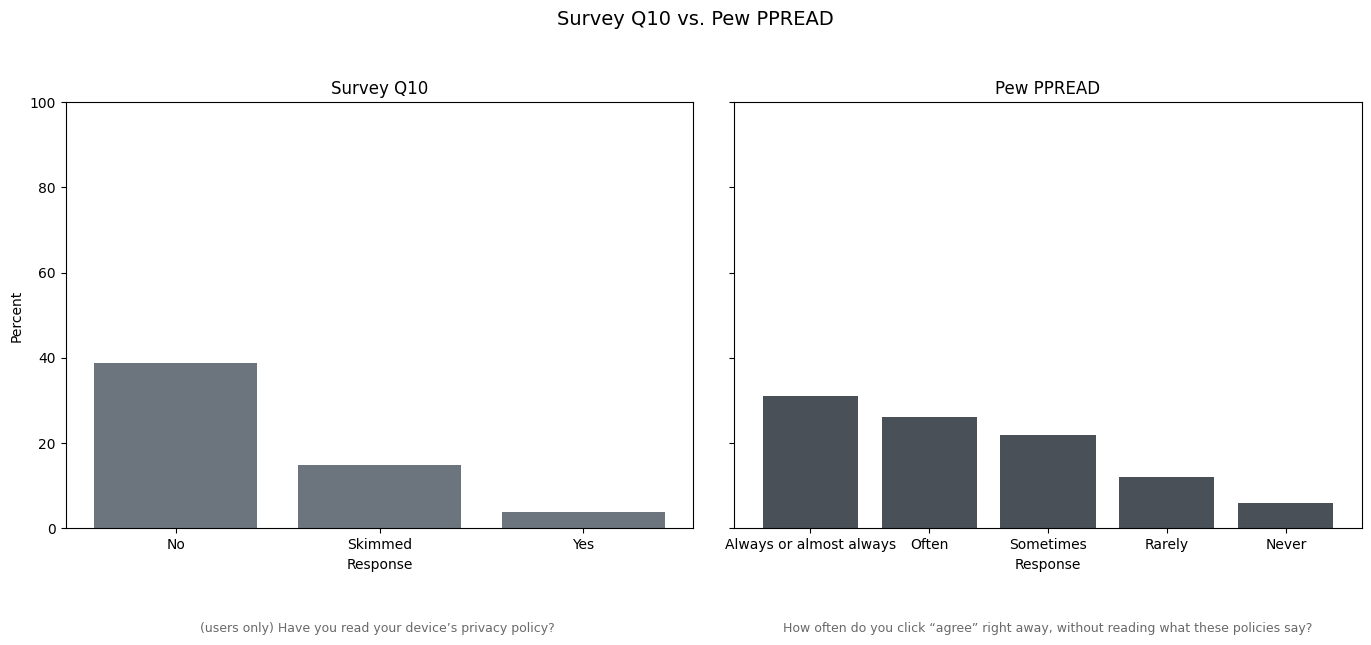
\includegraphics[width=1\linewidth]{figures/img/Pew_comparison_plots/compare_10_vs_PPREAD.png}
		\caption{Privacy Policy Engagement: Survey vs. Pew Research Center (2023)}
		\label{fig:Q10_Pew_comparison}
	\end{figure}
	Comparing these two datasets, substantive engagement with privacy policies is the exception rather than the rule. In both samples, the majority of individuals either do not read or only superficially engage with the terms that define how their data may be used, shared, or monetized. The thesis survey, with its focus on wearable health devices, reveals even lower rates of full reading than the broader Pew sample, though the difference in question framing and context should be noted.
	\subsubsection{Behavioral Trade-offs: Health vs. Privacy}
	% Balancing health benefits and privacy concerns (Q8)
	Analysis of the health-privacy trade-off (Q8) reveals that users often prioritize or equally value health benefits over privacy. As shown in Figure~\ref{fig:Q8_tradeoff}, a majority of users are either "Equally concerned about both" or find that health benefits "somewhat" or "clearly" outweigh privacy concerns. The view that "Privacy concerns clearly outweigh health benefits" is the least common response, suggesting a pragmatic calculus among device users.
	\begin{figure}[ht]\centering
		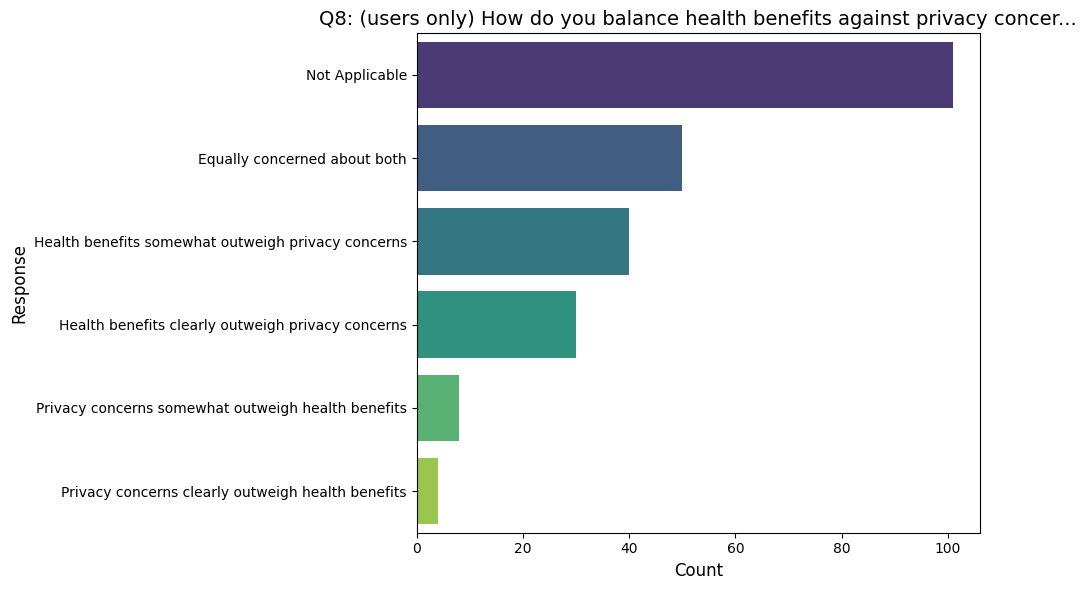
\includegraphics[width=1\linewidth]{figures/questions/Q8_single_choice.png}
		\caption{Trade-off Between Health Benefits and Privacy Concerns (Q8, device users only)}
		\label{fig:Q8_tradeoff}
	\end{figure}
	This trade-off is associated with attitudinal and demographic profiles. Attitudinal factors are influential. For instance, a higher privacy concern score is negatively correlated with prioritizing health benefits ($r = -0.31$, $p < 0.001$), indicating that as concern rises, the willingness to trade privacy for health diminishes. Conversely, higher trust in technology is positively correlated with prioritizing health benefits ($r = 0.17$, $p < 0.01$). The two user clusters also show a clear divergence: \textit{Pragmatic Sharers} are positively correlated with health-benefit-oriented responses, while \textit{Skeptics} are negatively correlated. Interestingly, a stronger preference for control is positively correlated with being "Equally concerned about both" ($r = 0.20$, $p < 0.01$), suggesting that a desire for agency is linked to a more balanced, rather than dismissive, view of privacy.
	Demographic factors also play a role, but a more modest one. Younger users and students are more likely to prioritize health benefits, with the 18--24 age group ($r = 0.27$, $p < 0.001$) and student occupation ($r = 0.24$, $p < 0.001$) both showing positive correlations with the view that "Health benefits somewhat outweigh privacy concerns." Language groups also show some variation; for example, French speakers are more likely to prioritize health benefits, while Spanish speakers tend to be more equally concerned. These subgroup distributions confirm that while the trade-off is a common feature of the user experience, its exact balance is shaped by a combination of underlying attitudes and demographic characteristics.
	\subsubsection{Device Usage Patterns}
	% User/non-user split, frequency, brand/app usage

	\paragraph{User/Non-User Split}
	Analysis of device usage (Q5) indicates that a majority of respondents (57.6\%) use or have used connected health devices.
	Several factors show statistically significant correlations with device usage. The \textit{tech trust score} ($r = 0.16$, $p < 0.05$) and \textit{control preference score} ($r = 0.13$, $p < 0.05$) are positively correlated with usage, indicating that higher trust and a greater preference for control are associated with being a device user. Conversely, \textit{privacy concern score} is negatively correlated with usage ($r = -0.15$, $p < 0.05$), suggesting higher privacy concerns are associated with non-use.
	Demographic factors also reveal distinct patterns. Device usage is highest among the 18--24 age group (73.5\%) and shows a significant negative correlation with the 65+ age group ($r = -0.14$, $p < 0.05$). Education level is also a factor, with usage being positively correlated with having a Bachelor's degree ($r = 0.15$, $p < 0.05$) and negatively correlated with having Upper Secondary/High School or Vocational training ($r = -0.13$, $p < 0.05$ for both). Among language groups, German speakers show a significant negative correlation with usage ($r = -0.17$, $p < 0.05$).
	The cluster profiles demonstrate the strongest associations with device usage, apart from the definitional \textit{user type}. The \textit{Pragmatic Sharers} profile is positively correlated with usage ($r = 0.29$, $p < 0.001$), while the \textit{Skeptics} profile has an equally negative correlation ($r = -0.29$, $p < 0.001$). The subgroup distribution report confirms these trends, showing that 65.9\% of Pragmatic Sharers are users, compared to only 32.2\% of Skeptics.

	\paragraph{Frequency of Device Usage}
	Among device users, engagement is high, with a majority (65.4\%) reporting 'Daily' usage. This high-frequency engagement is not uniform across the sample and correlates significantly with several attitudinal and demographic factors, as seen in Figure~\ref{fig:Q9_usage_frequency}.
	\begin{figure}[ht]\centering
		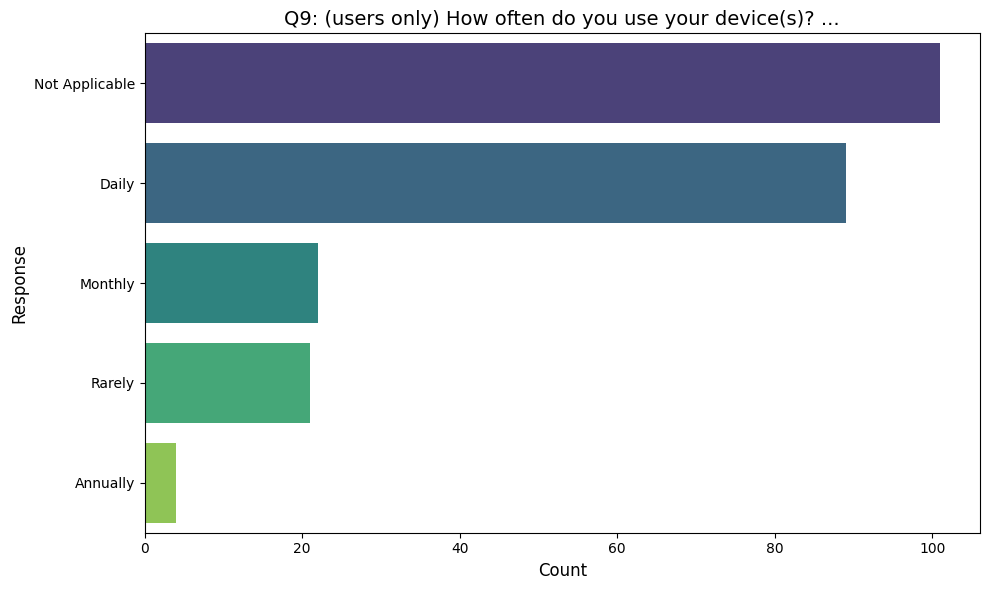
\includegraphics[width=1\linewidth]{figures/questions/Q9_single_choice.png}
		\caption{Device Usage Frequency Among Users (Q9)}
		\label{fig:Q9_usage_frequency}
	\end{figure}
	Attitudinally, daily usage is positively correlated with a higher \textit{tech trust score} ($r = 0.18$, $p < 0.01$) and negatively correlated with a higher \textit{privacy concern score} ($r = -0.21$, $p < 0.01$). Subgroup distributions confirm this: 88.9\% of users with the highest tech trust score use their device daily, compared to only 37.5\% of those with the lowest trust. Conversely, daily usage drops as privacy concern increases.
	The user clusters show a strong and polarized relationship with usage frequency. The \textit{Pragmatic Sharers} cluster is significantly and positively correlated with daily usage ($r = 0.22$, $p < 0.001$), while the \textit{Skeptics} cluster shows an equally strong negative correlation ($r = -0.22$, $p < 0.001$).
	Demographic factors also play a significant role. The 18--24 age group is positively correlated with daily usage ($r = 0.21$, $p < 0.01$), with 84\% of users in this bracket reporting daily use. Language is also a discriminant: English speakers are more likely to be daily users ($r = 0.16$, $p < 0.05$), whereas German speakers are less likely ($r = -0.16$, $p < 0.05$). Infrequent ('Rarely') usage is weakly but significantly correlated with being a Spanish speaker ($r = 0.13$, $p < 0.05$), holding a Bachelor's degree ($r = 0.15$, $p < 0.05$), and being self-employed ($r = 0.16$, $p < 0.05$).

	\paragraph{Brands}
	The wearable device market within the user sample is highly concentrated, with Apple (40.9\%) and Garmin (23.4\%) being the most frequently reported brands (see Figure~\ref{fig:Q7_brand_app}). This brand preference is not random but correlates significantly with specific attitudinal and demographic profiles.
	\begin{figure}[ht]\centering
		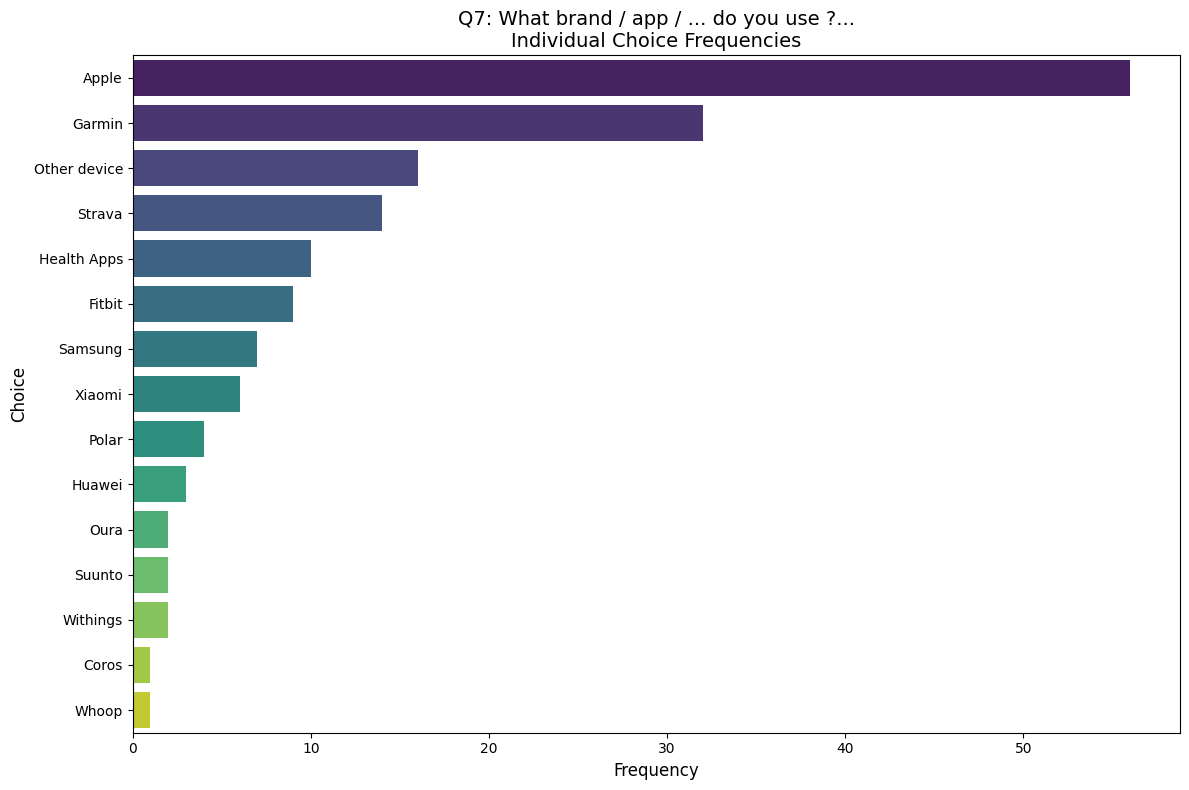
\includegraphics[width=1\linewidth]{figures/questions/Q7_multiple_choice.png}
		\caption{Brand and App Usage Among Device Users (Q7, multiple responses allowed)}
		\label{fig:Q7_brand_app}
	\end{figure}
	\begin{itemize}
		\item \textbf{User clusters:} The \textit{Pragmatic Sharers} cluster is significantly and positively correlated with using Apple ($r = 0.20$, $p < 0.01$) and Garmin ($r = 0.14$, $p < 0.05$). Conversely, the \textit{Skeptics} cluster shows an equally strong negative correlation with these two dominant brands.
		\item \textbf{Attitudes:} Garmin users show a significant negative correlation with both privacy concern score ($r = -0.16$, $p < 0.05$) and data ownership belief ($r = -0.15$, $p < 0.05$). In contrast, users of Fitbit and Xiaomi exhibit a positive correlation with a stronger belief in data ownership ($r = 0.15$ and $r = 0.13$, respectively; $p < 0.05$).
		\item \textbf{Demographics:} Apple is more prevalent among the 25--34 age group ($r = 0.15$, $p < 0.05$), while its usage is negatively correlated with the 45--54 age group ($r = -0.15$, $p < 0.05$). Spanish-speaking users are significantly less likely to use Garmin ($r = -0.17$, $p < 0.01$) and more likely to use 'Other device' ($r = 0.20$, $p < 0.01$). Occupation also plays a role; for instance, self-employed individuals are strongly correlated with using 'Other device' ($r = 0.27$, $p < 0.001$) and negatively correlated with using Apple ($r = -0.14$, $p < 0.05$).
	\end{itemize}
\subsection{Axis 4: Innovative Technologies and Future Directions}
	\subsubsection{Awareness of Decentralized Technologies}
		Awareness of decentralized data management approaches, such as blockchain or personal data vaults, is limited across the sample. A plurality of respondents (48.3\%) report being “No, not familiar” with these technologies, while 42.4\% are “somewhat familiar,” and only 9.2\% are “very familiar.” This knowledge gap, however, is not uniform and shows significant variation across specific demographic subgroups.
		Familiarity is positively correlated with being a device user. Users are significantly more likely to report being “very familiar” with these concepts than non-users ($r = 0.16$, $p < 0.05$), with subgroup data showing 13.1\% of users in this category compared to just 4.0\% of non-users.
		Education level presents a pattern as well. Respondents with “Vocational/Technical training or certificate” show a significantly higher level of awareness, being positively correlated with being “very familiar” ($r = 0.17$, $p < 0.01$). This group has the highest proportion of “very familiar” individuals (19.1\%) and the lowest proportion of those “not familiar” (29.8\%). Conversely, those with a Doctorate (PhD) report the highest rate of being “not familiar” (80\%).
		Language and occupation also act as differentiators. German speakers are significantly more likely to be familiar with these technologies than other language groups ($r = 0.16$, $p < 0.05$), with only 22.7\% reporting they are “not familiar,” compared to 59.2\% of Spanish speakers. Self-employed individuals are also more likely to be “very familiar” with decentralized approaches ($r = 0.15$, $p < 0.05$). No significant correlations are observed with attitudinal variables like privacy concern, tech trust, or control preference.
	\subsubsection{Trust in New Technologies}
		% Trust in blockchain-based systems (Q13), by education
		Trust in new decentralized technologies, such as blockchain, to protect wearable health data is characterized by a pronounced neutrality across the sample. The mean trust score is 3.01 on a five-point scale, with a plurality of respondents (40.8\%) selecting the neutral midpoint. While a slightly larger share expresses some level of trust (32.3\%) over distrust (26.9\%), high trust is rare (4.6\%), as seen in Figure~\ref{fig:Q13_trust_newtech}.
		\begin{figure}[ht]\centering
			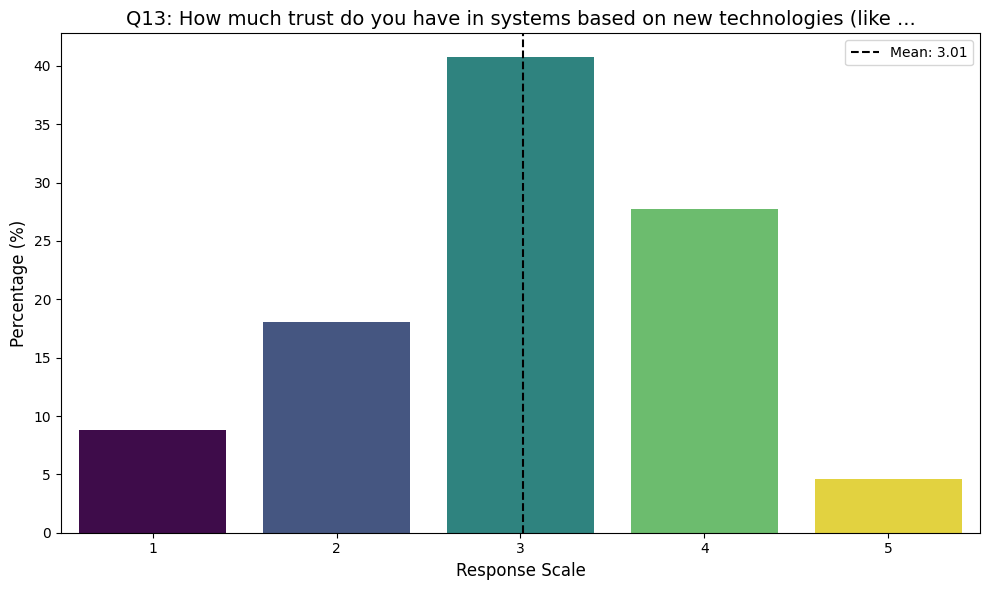
\includegraphics[width=1\linewidth]{figures/questions/Q13_likert.png}
			\caption{Distribution of Trust in New Technologies (Q13: 'I trust systems based on new technologies (e.g., blockchain) to protect my wearable health data')}
			\label{fig:Q13_trust_newtech}
		\end{figure}
		This ambivalent stance is not uniform and is significantly correlated with key attitudinal profiles. The strongest predictor of trust is privacy concern, which exhibits a moderate negative correlation ($r = -0.34$, $p < 0.001$). Subgroup analysis confirms this starkly: 100\% of respondents with the lowest privacy concern express trust, whereas 80\% of those with the highest concern express distrust. Conversely, a higher preference for control is correlated with higher trust in new technologies ($r = 0.33$, $p < 0.001$).
		The user clusters also show a significant and polarized relationship. The \textit{Pragmatic Sharers} cluster is positively correlated with trust ($r = 0.26$, $p < 0.001$), while the \textit{Skeptics} cluster is negatively correlated ($r = -0.26$, $p < 0.001$). This aligns with the finding that device users are significantly more likely to trust these technologies than non-users ($r = 0.16$, $p < 0.05$).
		Demographic factors play a lesser, though significant, role. The 25--34 age group shows a positive correlation with trust ($r = 0.15$, $p < 0.05$), while the 55--64 age group shows a negative correlation ($r = -0.17$, $p < 0.05$). Notably, respondents with a Doctorate (PhD) report the highest levels of distrust, with 40\% selecting the lowest trust score.
	\subsubsection{Trust in New Technologies: Survey vs. Pew}

	\paragraph{Trust in New Technologies: Survey vs. Pew}
	The Pew benchmark, asked respondents about their trust in companies to make responsible decisions regarding artificial intelligence in their products. While this question is broader than our specific focus on blockchain or decentralized systems, it taps into the same underlying concerns about technological stewardship and institutional accountability. The Pew results paint a picture of pronounced skepticism. Only 2\% of respondents report "a great deal" of trust—a strikingly small fraction. Another 22\% indicate "some" trust, while the vast majority express reservations: 41\% select "very little" trust and 30\% choose "not at all." In total, an overwhelming 71\% of respondents harbor little to no trust in companies' handling of AI. Trust, it seems, is in short supply.
	Our thesis sample tells a somewhat different story. As we've seen, neutrality dominates the landscape.
	Figure~\ref{fig:trust_newtech_Pew} brings this comparison into visual focus, overlaying our survey results with the 2023 Pew Research Center data. The graph reveals that across both populations, high confidence in new technologies is rare, and most respondents cluster at the neutral or Skeptics end of the spectrum.
	\begin{figure}[ht]\centering
		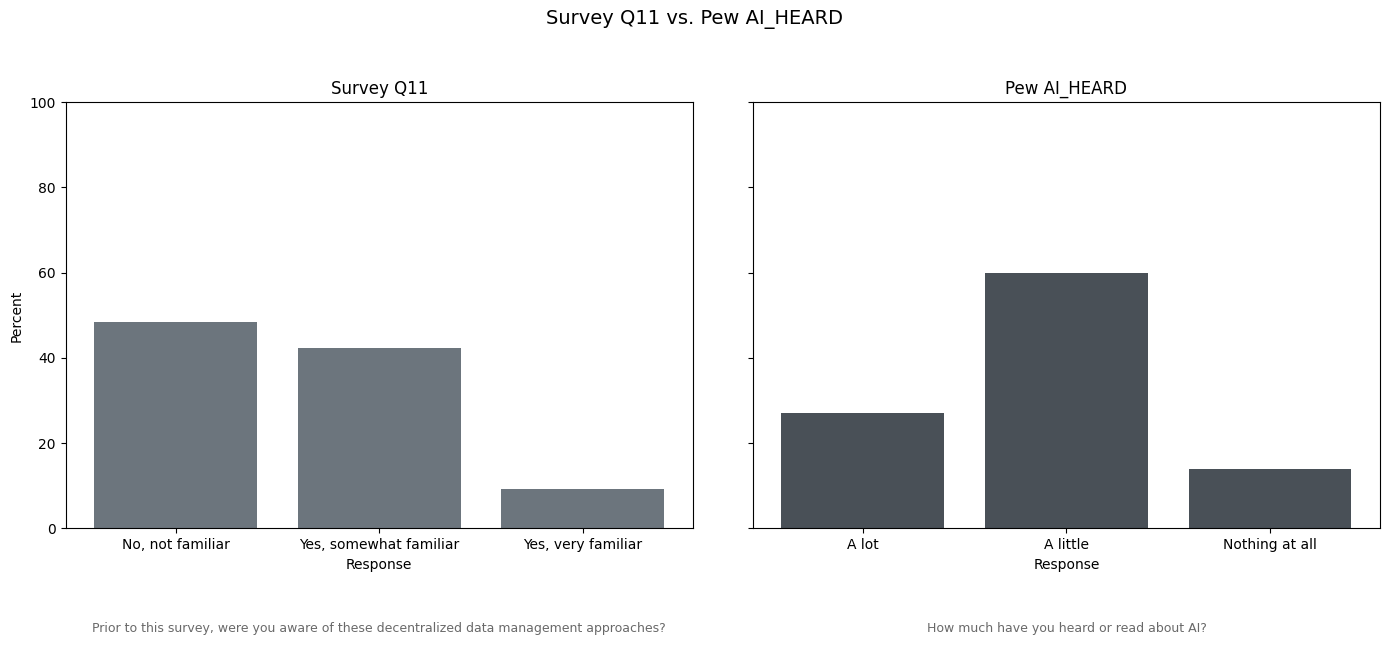
\includegraphics[width=1\linewidth]{figures/img/Pew_comparison_plots/compare_11_vs_AI_HEARD.png}
		\caption{Trust in New Technologies: Survey Sample vs. Pew Research Center (2023)}
		\label{fig:trust_newtech_Pew}
	\end{figure}
	The visual comparison highlights two distinct response patterns: our sample's "wait and see" neutrality versus the Pew respondents' more pronounced skepticism. But few people in either group express strong confidence in emerging technological systems, suggesting a fundamental wariness. 			
	In sum, both datasets tell us that strong trust in emerging technological systems—whether decentralized architectures or AI-driven platforms—is the exception rather than the rule.
	\subsubsection{Willingness to Pay or Invest}
	% Willingness to pay/invest for decentralized solutions (Q15)
	Willingness to invest time or money in decentralized data solutions is limited across the sample, with a mean score of 2.69 on a five-point scale. A plurality of respondents (30.7\%) are neutral, but a larger combined share expresses unwillingness (44.5\% selecting scores 1 or 2) than willingness (24.8\% selecting scores 4 or 5), as seen in Figure~\ref{fig:WTP_distribution}. 
	\begin{figure}[ht]\centering
		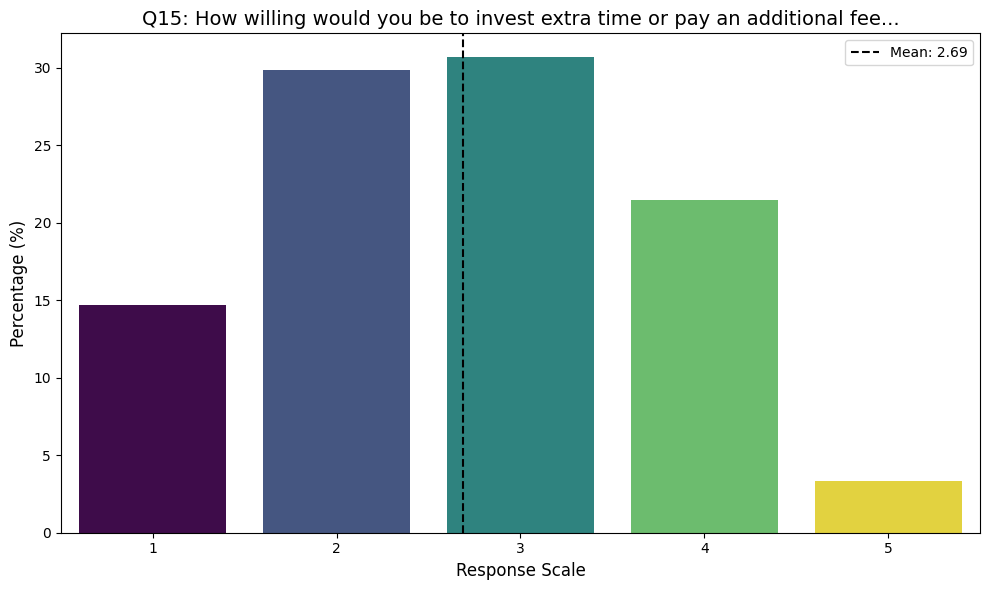
\includegraphics[width=1\linewidth]{figures/questions/Q15_likert.png}
		\caption{Distribution of Willingness to Pay or Invest in Decentralized Data Solutions (Q15)}
		\label{fig:WTP_distribution}
	\end{figure}
	This general reluctance, however, is not uniform and is shaped by attitudinal factors.
	The single most dominant predictor is control preference, which exhibits a strong positive correlation with willingness to pay ($r = 0.76$, $p < 0.001$). The subgroup analysis confirms this: 100\% of respondents with the lowest control preference are unwilling to pay, while 100\% of those with the highest preference are willing. This indicates a direct relationship where the desire for control translates into a willingness to bear costs for solutions that provide it.
	Trust in new technologies is also a significant, though less powerful, positive predictor ($r = 0.27$, $p < 0.001$). Respondents with higher trust are more willing to invest, while those with the lowest trust are unwilling (57.1\% selecting score 1).
	The relationship with privacy concern is non-linear and does not appear as a significant linear correlation. Subgroup data shows that individuals with both the lowest and highest levels of privacy concern are the most unwilling to pay. For instance, 75\% of those with 'Low' concern and 50\% of those with the highest possible concern score selected the lowest willingness score. Willingness appears to peak among those with moderately high, but not extreme, levels of concern.
	Demographic factors play a minor role. Age shows a weak but significant pattern, with the 25--34 and 35--44 age groups being slightly more willing to invest, while older (45--54, 55--64) and younger (18--24) groups are less willing. Education level reveals a counterintuitive finding: respondents with a Doctorate (PhD) are the most unwilling to pay, with 80\% selecting scores of 1 or 2.		
	\subsubsection{Expectations for Mainstream Adoption}
		Expectations for the mainstream adoption of decentralized data management technologies within the next 5–10 years are generally optimistic. The mean response is 3.64 on a five-point scale, with a median of 4.0, indicating a tilt towards likelihood. A majority of respondents (57.1\%) believe adoption is "likely" or "very likely" (scores 4 or 5), while only 14.7\% view it as unlikely, as seen in Figure~\ref{fig:mainstream_adoption_expectation}. 
		\begin{figure}[ht]\centering
			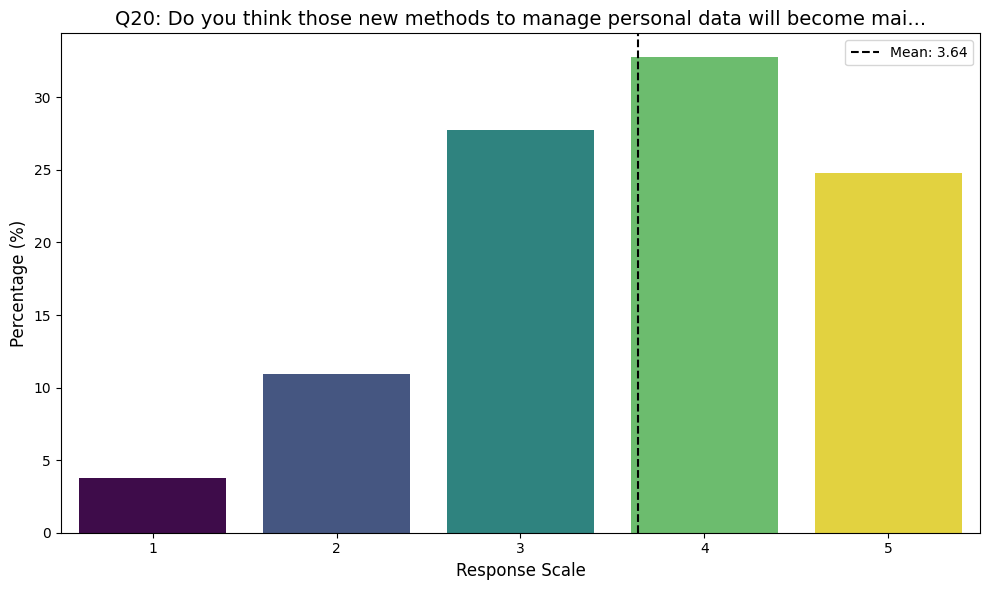
\includegraphics[width=1\linewidth]{figures/questions/Q20_likert.png}
			\caption{Expectations for Mainstream Adoption of Decentralized Data Management (Q20)}
			\label{fig:mainstream_adoption_expectation}
		\end{figure}
		This optimism, however, is not uniformly distributed and reveals significant patterns when analyzed by user cluster and demographics. The most interesting finding is the inverse relationship between cluster profile and expectation. The \textit{Skeptics} cluster, despite its general distrust, is positively correlated with expecting mainstream adoption ($r = 0.16$, $p < 0.05$). Conversely, the \textit{Pragmatic Sharers} cluster is negatively correlated with this expectation ($r = -0.16$, $p < 0.05$). Subgroup data confirms this: 37.3\% of Skeptics believe adoption is "very likely," compared to only 20.7\% of Pragmatic Sharers.
		Age also plays a significant role. The 55--64 age group shows the strongest positive correlation with expecting adoption ($r = 0.19$, $p < 0.01$), with 50\% of this group selecting the highest score. In contrast, the 25--34 age group ($r = -0.14$, $p < 0.05$) and students ($r = -0.19$, $p < 0.01$) are significantly less optimistic.
		Notably, core attitudinal variables such as privacy concern, control preference, and trust in new technologies do not show significant linear correlations with expectations for mainstream adoption. The subgroup distributions for these variables do not reveal a clear, monotonic trend, indicating that a respondent's general attitude toward privacy or technology does not directly predict their forecast for market-level adoption.
	\subsubsection{Barriers to Adoption}
		For barriers to adoption, the findings reveal that security and reliability concerns emerged as the most prominent barrier, with half of all respondents (50.6\%) expressing uncertainty about these fundamental aspects of decentralized systems, as seen in Figure~\ref{fig:Q14_barriers}. 
		\begin{figure}[ht]\centering
			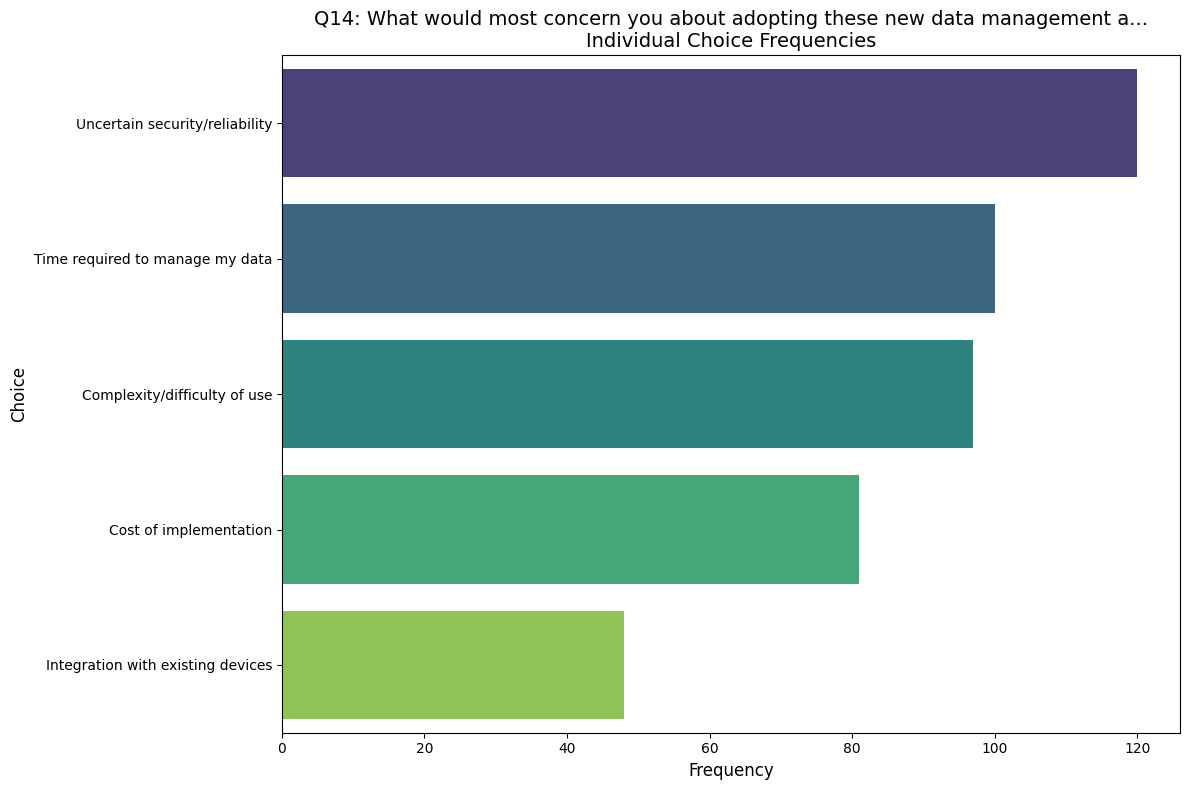
\includegraphics[width=1\linewidth]{figures/questions/Q14_multiple_choice.png}
			\caption{Barriers to adoption of decentralized data management (Q14)}
			\label{fig:Q14_barriers}
		\end{figure}
		This skepticism was particularly pronounced among individuals with heightened privacy concerns ($r = 0.31$, $p < 0.001$) and those exhibiting lower trust in technology ($r = -0.27$, $p < 0.001$).
		The time burden associated with personal data management represented the second most frequently cited barrier (42.2\%), revealing a preference for convenience over control among a substantial portion of users. Interestingly, this concern was more prevalent among respondents with lower privacy concern scores ($r = -0.16$, $p < 0.05$).
		Complexity and usability challenges was also important (40.9\%), with Spanish-speaking respondents demonstrating significantly less concern about system difficulty ($r = -0.21$, $p < 0.01$). 
		Cost considerations, while less universal, still affected over one-third of respondents (34.2\%), with Spanish speakers showing heightened sensitivity to implementation expenses ($r = 0.14$, $p < 0.05$). This pattern, combined with their lower concern about complexity, suggests distinct priorities within different cultural contexts regarding the evaluation of new technologies.
		Integration challenges with existing devices represented a notable concern for specific user segments, particularly affecting Pragmatic Sharers ($r = 0.22$, $p < 0.001$) and current device users ($r = 0.16$, $p < 0.05$), while being less relevant for Skeptics ($r = -0.22$, $p < 0.001$) and non-users ($r = -0.16$, $p < 0.05$). 
		Age-related patterns showed that older adults (65+) demonstrated greater security concerns ($r = 0.15$, $p < 0.05$), reflecting perhaps a more cautious approach to new technologies developed through years of experience with technological change. Conversely, younger adults (25-34) prioritized integration compatibility ($r = 0.20$, $p < 0.01$) while showing less concern about security ($r = -0.14$, $p < 0.05$).
		These findings collectively reveal that the path toward decentralized data management faces resistance not merely from technological limitations, but from a complex web of user priorities, demographic characteristics, and practical concerns.
\subsection{Advanced Analysis}
	\subsubsection{Factor Analysis and Principal Component Analysis}
	The empirical landscape mapped in the preceding analyses is, by design, multidimensional. While regression and correlation models have clarified the main axes of association among key variables, they do not fully capture the latent structure underlying user attitudes and behavioral intentions. To address this, a factor analysis and principal component analysis (PCA) were conducted, aiming to distill the complex web of survey responses into a smaller set of interpretable dimensions. This approach allows for a more nuanced understanding of how the various attitudinal and behavioral constructs coalesce, overlap, or diverge within the sample.

	\paragraph{Factor Extraction and Loadings}
	The rotated factor solution yielded three factors with eigenvalues above 1, together accounting for approximately 54\% of the total variance (Factor 1: 24\%, Factor 2: 18\%, Factor 3: 12\%). The factor loading matrix, visualized in Figure~\ref{fig:factor_loadings_heatmap}, reveals a structure with minimal cross-loading, supporting the empirical distinctiveness of the extracted dimensions.
	\begin{figure}[ht]\centering
		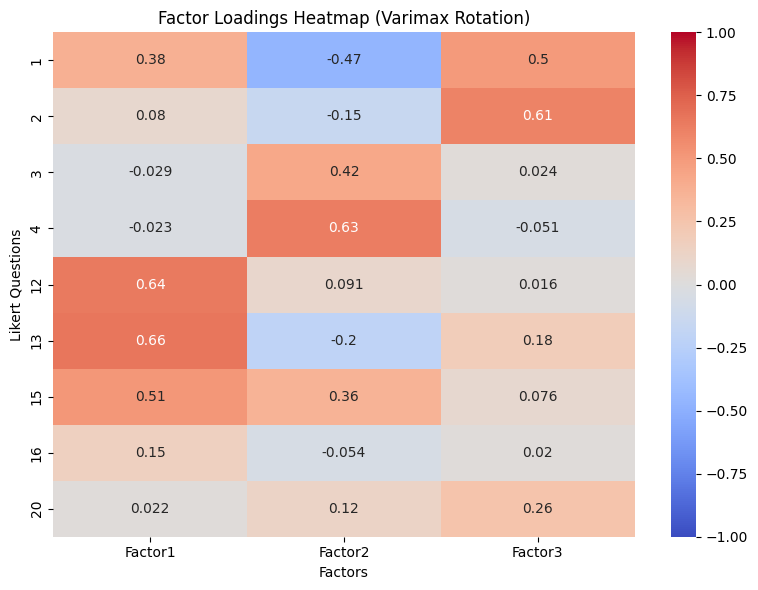
\includegraphics[width=1\linewidth]{figures/img/factor_analysis/factor_loadings_heatmap.png}
		\caption{Factor Loading Heatmap (Varimax, 3 Factors)}
		\label{fig:factor_loadings_heatmap}
	\end{figure}
	\textbf{Factor 1}, which explains the largest portion of the variance, is defined by high positive loadings from questions concerning the willingness to use systems that provide greater control (Q12: 0.64), trust in new technologies like blockchain (Q13: 0.66), and the willingness to invest time or money for such solutions (Q15: 0.51). This dimension empirically captures an orientation of \textit{Openness to and Trust in Decentralized Solutions}.
	\textbf{Factor 2} is principally anchored by strong positive loadings on privacy concern (Q4: 0.63) and the desired level of user control (Q3: 0.42). The co-location of these items indicates that privacy anxiety and a normative demand for agency are empirically intertwined, forming a distinct dimension of \textit{Privacy Concern and Desire for User Control}.
	\textbf{Factor 3} is characterized by high positive loadings on perceived control over data within current systems (Q2: 0.61) and trust in those same centralized systems (Q1: 0.50). This factor represents an individual's degree of \textit{Trust and Perceived Control in the Current System}.
	Other items, notably the belief in user data ownership (Q16) and expectations for mainstream adoption of new technologies (Q20), exhibit low communalities and do not load strongly on any of the three factors, indicating their empirical independence from these primary attitudinal constructs.

	\paragraph{Principal Component Analysis and Dimensional Independence}
	\begin{figure}[h!]\centering
		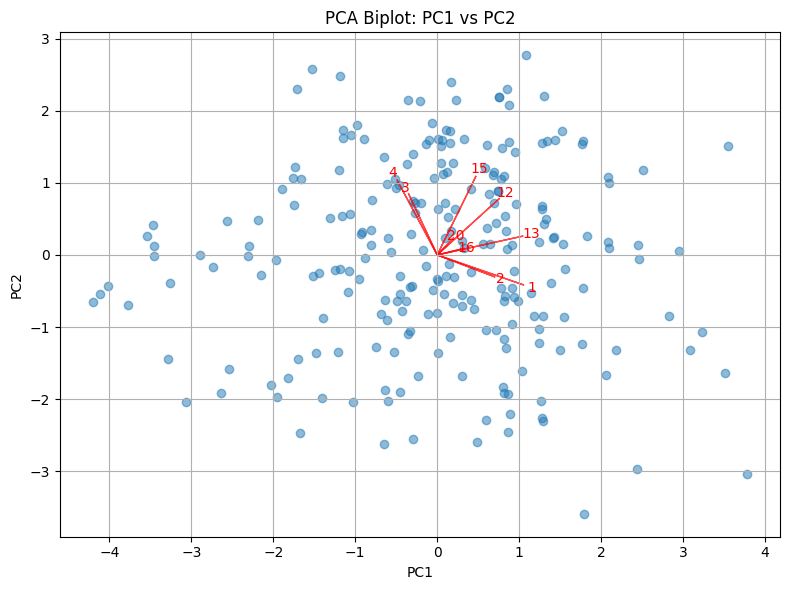
\includegraphics[width=0.7\linewidth]{figures/img/factor_analysis/pca_biplot_pc1_vs_pc2.png}
		\caption{PCA Biplot: PC1 vs. PC2}
		\label{fig:pca_biplot_pc1_vs_pc2}
	\end{figure}
	\begin{figure}[h!]\centering
		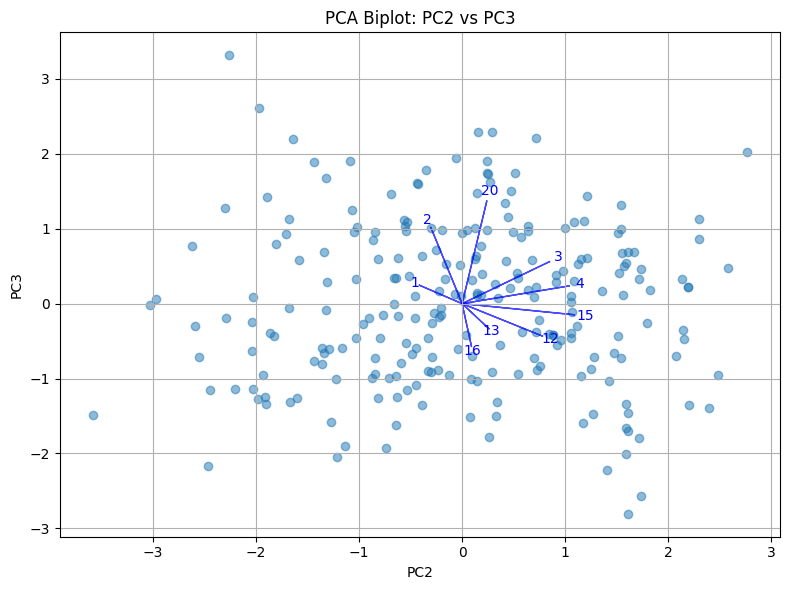
\includegraphics[width=0.7\linewidth]{figures/img/factor_analysis/pca_biplot_pc2_vs_pc3.png}
		\caption{PCA Biplot: PC2 vs. PC3}
		\label{fig:pca_biplot_pc2_vs_pc3}
	\end{figure}
	\begin{figure}[h!]\centering
		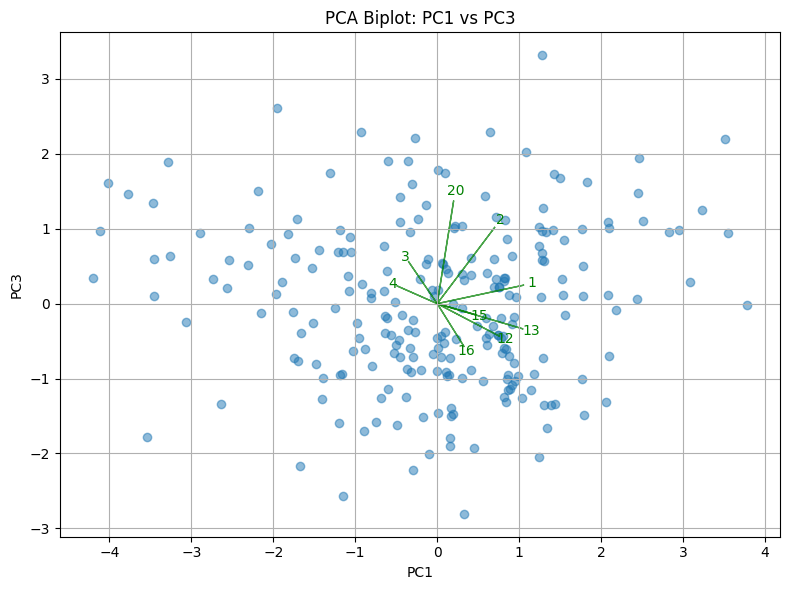
\includegraphics[width=0.7\linewidth]{figures/img/factor_analysis/pca_biplot_pc1_vs_pc3.png}
		\caption{PCA Biplot: PC1 vs. PC3}
		\label{fig:pca_biplot_pc1_vs_pc3}
	\end{figure}
	The PCA results reinforce the factor analytic structure. The scree plot (Figure~\ref{fig:scree_plot}) shows a clear inflection after the third component, supporting the retention of three principal axes. The first three components together explain just over half of the total variance, with diminishing returns for additional components.
	\begin{figure}[ht]\centering
		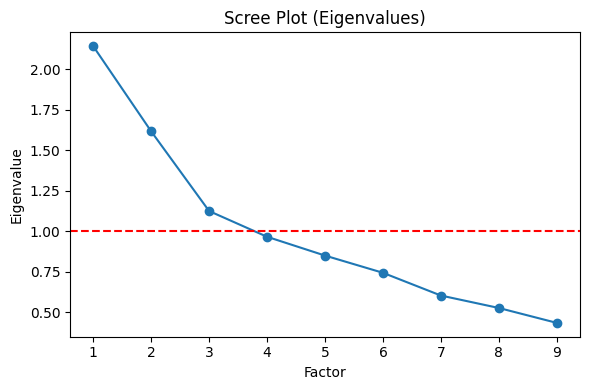
\includegraphics[width=0.7\linewidth]{figures/img/factor_analysis/scree_plot.png}
		\caption{Scree Plot of Eigenvalues (PCA)}
		\label{fig:scree_plot}
	\end{figure}
	The biplots of principal components (Figures~\ref{fig:pca_biplot_pc1_vs_pc2}, Figure~\ref{fig:pca_biplot_pc2_vs_pc3}, and Figure~\ref{fig:pca_biplot_pc1_vs_pc3}) provide a visual summary of the relationships among items and components. And provide a visual confirmation of the independence of these components. The vectors representing the survey items radiate outwards from the origin in a star-like pattern rather than clustering, which indicates that the underlying dimensions are largely orthogonal. For instance, the biplot of PC1 versus PC2 shows that items loading on Factor 1 (Q12, Q13, Q15) project strongly along the PC1 axis, while items from Factor 2 (Q3, Q4) project primarily along the PC2 axis, confirming their distinctness. This geometric independence suggests that user attitudes are not reducible to a single dimension but are composed of multiple, non-overlapping constructs.
	\subsubsection{Structural Equation Modeling}
	Each preceding approach has contributed a distinct perspective on the relationships among privacy concern, control preference, trust in technology, data ownership belief, and behavioral intentions regarding wearable health data. To further interrogate the latent structure underlying these constructs and to test the plausibility of directional relationships among them, a structural equation modeling (SEM) approach was employed. This subsubsection details the rationale, model specification, estimation procedures, and empirical findings of the SEM analysis, while maintaining a focus on transparency and methodological rigor.

	\paragraph{Empirical Findings: Structural Model}
	The estimation of the structural model converged successfully; however, the analysis did not find statistically significant path coefficients for the hypothesized directional relationships. The direct effect of \texttt{factor\_privacy} on \texttt{factor\_openness} was estimated at $0.00$ (SE $= 0.05$, $z = 0.00$, $p = 1.0$). Similarly, the path from \texttt{factor\_privacy} to \texttt{factor\_control} was non-significant, with an estimated coefficient of $0.00$ (SE $= 0.05$, $z = 0.00$, $p = 1.0$). The path from \texttt{factor\_control} to \texttt{factor\_openness} was also estimated at $0.00$ (SE $= 0.06$, $z = 0.00$, $p = 1.0$).
	While the structural paths were non-significant, the variances of the latent constructs themselves were statistically significant, indicating internal consistency. The variance for \texttt{factor\_control} was estimated at $0.39$ ($p < 0.001$) and for \texttt{factor\_openness} at $0.33$ ($p < 0.001$). The bootstrapped confidence intervals for all structural path coefficients were wide and included zero, reinforcing the lack of statistical significance. These results empirically confirm the pattern of independence among the three core attitudinal dimensions that was previously suggested by the EFA and PCA, indicating that, within this dataset, the constructs operate as parallel rather than causally linked phenomena.

\section{Discussion}
\subsection{Synthesizing the Empirical Findings: A Portrait of the Contemporary Wearable User}
	% This section requires a high-level summary of the core empirical narrative. The selected sources establish the central tension: users are concerned, feel a lack of control, yet desire control and are open to innovation. They also introduce the two key user segments that challenge a monolithic view of the "user," which is a stated goal of this subsection.
	The empirical findings reveal a significant privacy concern among users of wearable devices, demonstrating a fundamental tension with the frictionless data flows idealized by Dataism. This concern, while not homogeneous across the sample, constitutes a core dimension of user identity formation. Two distinct attitudinal profiles emerge from the analysis: 'Skeptics,' who exhibit fundamental distrust and resistance toward the incumbent centralized paradigm, and 'Pragmatic Sharers,' who engage in a calculated benefit-risk evaluation prior to data disclosure. Notably, privacy anxieties stem predominantly from anticipated data misuse and technological distrust, rather than abstract notions of digital sovereignty. This insight provides crucial context for understanding the privacy paradox—the discrepancy between stated privacy values and actual disclosure behaviors. While broader societal data confirms the pervasiveness of these concerns, they manifest with diminished intensity in the health wearable domain due to perceived utilitarian benefits. Nevertheless, this anxiety engenders a substantial trust deficit, presenting a significant barrier for centralized data governance models and motivating exploration of alternative paradigms that enhance user agency.
	The empirical data further demonstrates that a majority of users perceive themselves as having negligible control over their personal data. This finding provides robust empirical validation for the literature's critique of eroded user agency in digital environments. A pronounced disconnect exists between the industry's empowerment narrative and the lived reality where users function primarily as passive data sources rather than sovereign actors. This agency deficit catalyzes heightened privacy anxiety, establishing a self-reinforcing cycle of disempowerment and distrust that transcends demographic and behavioral segments. The near-universal nature of this experience, affecting both \textit{Pragmatic Sharers} and \textit{Skeptics} alike, suggests a systemic failure of the current centralized model rather than a segment-specific phenomenon—a conclusion substantiated by external comparative data confirming this control deficit as a widespread societal baseline.
	Conversely, the data reveals an overwhelming and remarkably consistent demand for enhanced agency across demographic and behavioral strata. The pronounced preference for "High" or "Complete" control over personal data creates a stark disjunction between current perceived powerlessness and normative expectations of digital sovereignty. This desire for control exhibits a strong positive correlation with privacy anxiety, intensifying proportionally with concerns regarding potential data misuse. The statistical independence of this agency demand from technology trust and data ownership beliefs isolates it as a visceral response to the inadequacies of the current centralized paradigm, framing the willingness to adopt alternative solutions not merely as technological curiosity but as a direct pursuit of reclaimed autonomy.
	Despite prevailing privacy concerns and perceptions of disempowerment, the research identifies significant openness to innovative solutions that promise enhanced user agency. This receptivity is primarily driven by control preference and trust in emergent technological paradigms rather than mere technological enthusiasm. The empirical analysis suggests a nuanced relationship between privacy attitudes and adoption intentions: while elevated privacy concern inhibits data sharing within the current centralized framework, the promise of tangible control may redirect this same concern toward constructive interest in user-centric alternatives. This dynamic manifests in the divergent responses of 'Pragmatic Sharers,' who perceive decentralized systems as vehicles for enhanced empowerment, and 'Skeptics,' whose fundamental distrust remains a significant adoption barrier. These findings tentatively suggest that the future of data governance frameworks is one that prioritizes authentic, user-centric control mechanisms rather than abstract privacy assurances.
\subsection{Answering the Research Questions}
% This section is now explicitly structured to answer each research question sequentially, connecting the empirical results from the previous chapter to the theoretical frameworks and literature.
	\subsubsection{Addressing the Primary Research Question: Evaluating Decentralized Solutions}
	% This subsubsection directly answers the Primary RQ. It discusses how users evaluate decentralized technologies as a solution to the ethical, privacy, and autonomy challenges of Dataism. It will argue that while users are open to these solutions, their evaluation is primarily driven by a desire for control (a key factor), rather than a deep understanding of the technology itself. It will synthesize the regression and factor analysis results to pinpoint 'control preference' and 'tech trust' as the most influential factors for adoption.

	\paragraph{Privacy Concern}
	The empirical findings on willingness to adopt decentralized solutions provide a direct answer to the primary research question, revealing that users evaluate these innovations as potential instruments for reclaiming digital sovereignty. The exploratory regression results indicate that, within this sample, preference for greater control is a comparatively stronger correlate of stated adoption willingness than privacy concern. This pattern may motivate a refinement (rather than a wholesale reframing) of how the privacy calculus is modeled, pending replication. This dynamic is validated by the polarization between the 'Pragmatic Sharers,' who see such systems as a logical step toward greater empowerment, and the 'Skeptics,' whose fundamental lack of trust remains a significant barrier. Ultimately, the willingness to adopt is less a reaction against privacy loss and more a proactive pursuit of agency, indicating that the most viable path forward for data governance is one that places user-centric control at its core.

	\paragraph{Perceived Control Over Data}
	However, this evaluation process is constrained by a significant knowledge gap, as the empirical data reveals a low baseline awareness of decentralized technologies across the sample. This unfamiliarity represents a primary obstacle, suggesting that the potential for these solutions to counter the rising Dataist paradigm is largely unrealized because users cannot demand or adopt alternatives they do not know exist. The analysis further show that awareness levels do not correlate with key attitudinal drivers like privacy concern or the desire for control. This implies that even the users most motivated to seek alternatives may be unaware that such solutions are emerging, reinforcing the argument that user education is an important prerequisite for adoption. While small pockets of higher awareness exist among specific subgroups, such as those with vocational training or current device users, the overall landscape is one of non-awareness, indicating that the "latent demand" for digital sovereignty is predicated on a level of technical literacy that is not yet widespread.

	\paragraph{Willingness to Adopt}
	Furthermore, the evaluation of these new technologies is shaped by a complex and often contradictory calculus of trust. The empirical data reveals that trust in decentralized solutions is not a given, but is characterized by a widespread neutrality, reflecting a "wait-and-see" attitude likely born from low awareness. This ambivalence is the result of two powerful, opposing forces. While high privacy concern dilutes confidence in any data-handling system, new or old, a proactive desire for control actively builds it. The regression analysis confirms that the promise of empowerment is as strong a positive driver for trust as privacy anxiety is a deterrent. This finding is interesting, as it suggests that overcoming user skepticism is less about assuaging abstract fears and more about providing concrete mechanisms for digital sovereignty, framing these technologies not as a defense against risk, but as an instrument for empowerment.
	\subsubsection{Addressing SRQ1: Centralized vs. Decentralized Models - A Comparative Analysis}
	% This subsubsection focuses on Secondary RQ1. It explicitly compares user attitudes towards the two models. It will contrast the low trust and low perceived control in centralized systems (Q1, Q2) with the high willingness to adopt (Q12) and higher trust in new technologies (Q13) when they promise control. This section directly addresses the comparative aspect of user trust, perceived benefits (control), and adoption willingness.

	\paragraph{Trust in Centralized Systems}
	The comparative analysis begins with the centralized model, which is defined by a significant and common trust deficit. The empirical data reveals a low level of trust in centralized data handlers, a finding that challenges the foundational principles of Dataism and validates the literature's consensus that trust is a fragile precondition for data sharing. This sentiment is not an isolated attitude but is linked with privacy anxiety. The negative correlation between the two suggests they are two sides of the same coin in the user's mind. This lack of trust appears to be a generalized sentiment, influenced more by a user's broad faith in the technological ecosystem than by a detailed evaluation of specific platforms, a dynamic indicative of "privacy fatigue." External comparisons with broader societal data confirm that this scarcity of high trust is a common phenomenon, establishing a low-trust baseline that represents a market failure for the centralized model and serves as a primary driver for exploring the decentralized alternatives.

	\paragraph{Perceived Control Over Data}
	With the common feeling of having little to no control over personal data, as noted by the results, a powerful observed validation for the literature's critique of Dataism can be made. This finding quantifies the "erosion of user agency" \cite{VanDijck2014}, revealing a stark disconnect between the industry's narrative of empowerment and a lived reality where users feel more like passive data sources than sovereign actors. This lack of agency is not a passive sentiment but a primary driver of privacy anxiety, creating a cycle of distrust and disempowerment that a general faith in technology is insufficient to overcome. Most importantly, this feeling of powerlessness is a near-universal experience that goes beyond user segments, affecting both engaged \textit{Pragmatic Sharers} and cautious \textit{Skeptics} alike. This pattern could reflect structural limitations or perceived shortcomings in current centralized arrangements. However, causality or systemic “failure” cannot be inferred from cross‑sectional, self‑reported data.

	\paragraph{Desired Control Over Data}
	This sense of disempowerment is directly countered by a near unanimous and demand for greater agency, which stands as a powerful pushback to any notion of user apathy. The preference for "High" or "Complete" control over personal data is not a niche sentiment but a remarkably consistent demand, highlighting a perceived gap between current experiences of control and respondents’ normative preferences regarding data governance. This desire for control is by nature linked to privacy anxiety, intensifying as concern over data misuse grows. The fact that this demand for agency operates independently of general tech trust or abstract beliefs in data ownership further isolates it as a core, instinctive response to the inadequacies of the current centralized model, framing the willingness to adopt new solutions as a direct pursuit of reclaiming lost control.

	\paragraph{Willingness to Adopt}
	Finally, this landscape of concern and disempowerment does not end up in indifference, but in a willingness to adopt new solutions, provided they restore user agency. This openness to innovation is primarily predicted by a user's preference for control and their trust in new technological ways of thinking. The regression analysis confirms by the numbers that the desire for control is a more influential driver of adoption than reactive privacy concerns. As explained before, this means that high privacy concern discourages sharing in centralized systems, but the promise of user control can motivate interest in decentralized alternatives, especially among those seeking empowerment rather than those who remain distrustful. 
	\subsubsection{Addressing SRQ2: Attitudinal and Structural Drivers and Barriers of Adoption}
	% This subsubsection tackles Secondary RQ2. It will detail the primary drivers for adoption, identified as control preference and tech trust. It will then analyze the main barriers identified in Q14 (security concerns, complexity, time), linking them to low prior awareness (Q11) and interpreting them in the context of the literature on usability and trust. It will also explicitly acknowledge that incentives were not directly measured, a limitation to be addressed later.

	\paragraph{Drivers for Adoption}
	The regression analysis provides an interesting answer to the second secondary research question regarding the factors that influence the adoption of decentralized technologies. The model suggests, subject to the limits of sample size and measurement, that control preference is a comparatively strong correlate of adoption intention. This finding supports the thesis's building argument, that in the coming age of Dataism, the path to user acceptance for new data mindsets is not about softening privacy fears, but about actively empowering users with tangible agency. The second most influential factor is trust in new technologies, which, while less powerful than control preference, still underscores that trust is important for adoption. The statistical significance of control preference and trust in new technologies positions digital sovereignty and confidence in innovation as the core pillars for adoption. These results offer an interesting distinction between reactive privacy concern and a proactive desire for control, suggesting that while high privacy concern may drive reluctance to share data within existing centralized systems, it does not, alone, translate into a willingness to adopt new ones. Instead, adoption is built on a constructive desire for control and a belief in the efficacy of new technological solutions, a finding that moves the discourse beyond the privacy paradox and toward a more nuanced understanding of user motivation.

	Furthermore, the factors influencing the adoption of these new technologies is shaped by a complex and often contradictory calculus of trust. The data collected reveals that trust in decentralized solutions is not a given, but is characterized by a common neutrality, reflecting a "wait-and-see" attitude which might be born from low awareness. This mixed feelings is the result of two powerful, opposing forces. While high privacy concern dilutes confidence in any data-handling system, new or old, a proactive desire for control actively builds it. The regression analysis confirms that the promise of empowerment is as strong a positive driver for trust as privacy anxiety is a deterrent. This finding is interesting, as it suggests that overcoming user skepticism is less about calming down abstract fears and more about providing concrete mechanisms for digital sovereignty, framing these technologies not as a defense against risk, but as an instrument for empowerment.

	\paragraph{Barriers to Adoption}
	However, significant barriers to adoption persist, rooted in the same anxieties that define the current centralized paradigm. The primary concerns cited by users (fear of data misuse, loss of privacy, security breaches, and a fundamental lack of control) are not abstract dealbreakers to technology but are rational responses to the perceived failures of the existing data governance model. These fears are the tangible expression of a broader privacy concern, with the feeling of disempowerment being a particularly big speed bump. This is validated by external data showing that nearly half the public has abandoned services over such issues, confirming that these barriers translate into concrete, market-shaping behavior. This landscape of distrust, particularly acute among \textit{Skeptics} (one of our segments), may raise the perceived threshold for new technologies, implying that decentralized solutions will need to demonstrate (to users) credible improvements in security and agency.

	Finally, as previously established in the portrait of the contemporary users section above, a foundational barrier is the widespread user unfamiliarity with decentralized technologies, which prevents even motivated individuals from considering these solutions.
	\subsubsection{Addressing SRQ3: The Role of Demographic and Behavioral Segmentation}
	% This subsubsection is dedicated to Secondary RQ3. It will analyze how demographic variables and the two identified user clusters (\textit{Pragmatic Sharers} and \textit{Skeptics}) influence attitudes. It will discuss the significant findings related to age, language group, and user type on variables like willingness to share, trust, and adoption intention, thereby providing a complete answer to the question of segmentation.
	Our analysis reveals significant demographic and behavioral patterns that shape user attitudes toward wearable technologies and data privacy. The collected evidence demonstrates a common privacy concern among participants, impacting the Dataistic assumption that information should flow freely without restriction. This concern, however, manifests unevenly across our sample, taking shape into two distinct attitudinal profiles that we have designated \textit{Skeptics} and 'Pragmatic Sharers.' The former exhibit pronounced privacy anxiety and resistance to prevailing centralized data governance models, whereas the latter engage in calculated risk-benefit evaluations prior to disclosure decisions. Age emerges as a particularly influential variable in this segmentation, with older respondents demonstrating higher privacy vigilance, while younger participants and students display markedly reduced concern. This suggests a generational normalization of data sharing practices. When examining responsibility attribution patterns, we observe another divergence: 'Skeptics,' who tend to be older and inherently distrustful, advocate for individual data responsibility, reflecting their defensive posture toward institutional actors they perceive as untrustworthy. Conversely, 'Pragmatic Sharers,' typically younger and more technologically engaged, assign primary responsibility to device manufacturers, indicating an expectation of ethical stewardship from commercial providers. These fundamental attitudinal differences directly translate into sharing behaviors, with cluster membership appearing, in this dataset, at least as differentiating as several demographic variables. This requires, however, validation with stronger clustering structure. \textit{Pragmatic Sharers} willingly exchange personal data for perceived health insights, while \textit{Skeptics} exhibit pronounced reluctance stemming from systematic distrust. Looking toward innovative solutions, we find that desire for enhanced control represents the primary motivator for potential adoption of decentralized technologies across segments, with even privacy-conscious users demonstrating openness to alternatives that promise authentic agency. The \textit{Pragmatic Sharers} perceive such systems as mechanisms for enhanced empowerment, while \textit{Skeptics} maintain their characteristic wariness. The fundamental decision to adopt wearable devices itself reveals a segmentation pattern, with lower privacy concerns and higher technological trust correlating with usage, and younger, more educated demographics taking the center stage among users, which further confirms the division between \textit{Pragmatic Sharers} and 'Skeptics.' Among device adopters, we observe mainly a daily usage patterns associated with reduced privacy concern and elevated trust, indicating that for regular users, perceived benefits consistently outweigh perceived risks. This engagement intensity varies demographically, with younger users more likely to maintain daily device relationships and certain language groups (particularly German speakers) demonstrating reduced usage frequency, reflecting how cultural privacy perspectives tangibly impact behavior. Finally, brand selection itself operates as an expression of underlying privacy values, with market leaders like Apple and Garmin disproportionately favored by 'Pragmatic Sharers,' signaling comfort within established ecosystems, while \textit{Skeptics} actively avoid these dominant platforms, manifesting their resistance to mainstream data governance paradigms.
	\subsubsection{Addressing SRQ4: Privacy Paradox and Attitudinal Discrepancies}
	% How does the privacy paradox shape wearable users’ attitudes and actual behaviors toward decentralized data management?
	% This subsubsection will explicitly address the privacy paradox.

	\paragraph{Privacy Policy Engagement and the Privacy Paradox}
	The findings on privacy policy engagement reveal a pronounced manifestation of the privacy paradox. Empirical data show that an overwhelming majority of users (67.6\%) completely disengage from privacy policies, while only 6.6\% report reading them fully. This disengagement is shows a pattern as \textit{Pragmatic Sharers} are more likely to avoid policies, and younger cohorts are especially prone to ignoring these documents.
	External comparison with the 2023 Pew Research Center data confirms that this behavior is not isolated but a pervasive feature of digital interaction, adding tentative support to critiques of the notice-and-consent framework (subject to questionnaire design limits). Widespread non-engagement challenges theoretical models that assume rational, informed actors, and instead points to a structural failure: users, faced with opaque and non-negotiable terms in the Dataist paradigm, experience "privacy fatigue" and resort to perfunctory acceptance without meaningful review.

	\paragraph{Willingness to Share Data}
	This finding justifies the exploration of decentralized alternatives that plant privacy protection at the architectural level, rather than relying on a fundamentally broken consent model. The logistic regression results on willingness to share data reveal a manifestation of the privacy paradox, providing evidence that user behavior in centralized systems is primarily governed by reactive risk aversion rather than proactive agency-seeking. The overwhelming significance of \textit{privacy\_concern} as a negative predictor validates the privacy calculus literature, while the striking non-significance of \textit{control\_preference} shows a fundamental disconnect between users' abstract desires and actual sharing decisions. This distinction offers a powerful explanatory mechanism for the privacy paradox: users may express strong preferences for control in principle, yet find no meaningful outlet for this preference within current 'take it or leave it' sharing paradigms, causing them to default to decisions based purely on their level of privacy concern. The regression thus demonstrates that within the centralized model, sharing behavior is defined by what users fear losing (privacy) rather than what they hope to gain through agency (control), a defensive rather than aspirational calculus. This empirical finding provides an interesting baseline for understanding user motivation and highlights why decentralized technologies, explicitly designed to shift this calculus from risk mitigation to active empowerment, may represent a necessary evolution rather than a simple alternative approach to data governance.
	
	\paragraph{Health Privacy Tradeoff}
	The empirical investigation into the health-privacy tradeoff directly shows a manifestation of the privacy paradox, revealing how users actively negotiate competing values. The data demonstrates a normalization of privacy concessions among active wearable users, who display a willingness to prioritize perceived health benefits over data protection concerns, which is a behavioral pattern that validates the privacy calculus framework. This calculated compromise is governed by a wide range of intersecting factors where privacy concern functions as a significant stop sign, while technical trust acts as a facilitator of data sharing. The more complex relationship between control preferences and data ownership beliefs further illustrates the multidimensional nature of user decision-making, where abstract principles of digital sovereignty interact with practical considerations of utility. These dynamics manifest heterogeneously across the population, with \textit{Pragmatic Sharers} younger cohorts, and students exhibiting greater receptivity to health-benefit tradeoffs, while \textit{Skeptics} and older demographics maintain stronger privacy boundaries. This empirically documented divergence backs up the thesis's central argument that current centralized models have normalized privacy concessions among regular users while simultaneously generating resistance among significant population segments with heightened privacy concerns, diminished trust, or stronger data ownership convictions. This pattern of selective acceptance based on perceived utility perfectly wraps up the privacy paradox, where users' theoretical concerns about privacy become subordinated to immediate, tangible benefits in actual decision-making contexts.
\subsection{Broader Implications of the Findings}
	% This section moves from direct answers to the wider impact of the research.
	\subsubsection{Theoretical Implications}
	% This subsubsection will discuss how the thesis contributes to academic theory. It will propose a refined model of user decision-making that separates privacy concern (a driver for caution in current systems) from control preference (a driver for adopting new systems). It will argue for the empirical validation of 'digital sovereignty' as a user-centric concept, not just a theoretical one.
	The logistic regression findings on willingness to share data refine theoretical models of user decision-making in data sharing contexts, establishing a conceptual distinction between deterrent and motivational factors. The results bakc up the theoretical starting point that data sharing within centralized systems operates primarily as a reactive mechanism driven by risk assessment rather than proactive agency seeking. The non-significance of control preference in predicting sharing behavior, despite its proven importance in adoption of decentralized solutions, provides theoretical validation for a forked model of user decision-making. One where privacy concerns function as powerful dealbreakers within existing systems, while control preferences operate as distinct motivational constructs that do not mitigate perceived risks in the usual playbook. This theoretical advancement, as we have seen, directly addresses the "privacy paradox" by demonstrating that users' abstract desires for control find no practical outlet in current "take it or leave it" scenarios, forcing them to default to decisions based purely on concern levels. The model thus reframes user decision-making not as a single-dimension privacy calculus, but as a multi-dimensional construct where the current centralized recipe fundamentally restricts users to risk-averse, defensive postures defined by what they fear losing rather than what they hope to gain through agency. This theoretical refinement explains why decentralized technologies, by explicitly shifting this calculus from risk mitigation to empowerment, represent an interesting transformation of the decision-making framework itself.

	The other regression analysis on willingness to adopt new technologies transforms theoretical models of user decision-making by validating a conceptual distinction between reactive and proactive motivational constructs. The non-significance of privacy concern in predicting adoption intentions, despite its central role in dealbreaking data sharing, provides further theoretical validation for a dual-process decision framework where qualitatively different psychological mechanisms govern defensive versus aspirational behaviors. This distinction moves theoretical discourse beyond the simplified "privacy paradox" toward a more sophisticated model where user motivation operates through parallel but independent processes. Risk assessment in existing systems versus agency pursuit in novel paradigms. The statistical significance of control preference and tech trust establishes that adoption is theoretically rooted in constructive, forward-looking motivations rather than reactive concerns. The empirical independence of normative data ownership beliefs from behavioral adoption intentions further challenges theoretical assumptions about the relationship between ethical positions and practical choices, suggesting that adoption theory must distinguish between abstract principles and actionable preferences. These findings establish the theoretical foundation for reconceptualizing user decision-making as an interplay between distinct motivational systems, providing a more nuanced explanatory framework that accounts for the apparent contradictions in how users evaluate and respond to different technological paradigms.

	The last regression analysis on trust in new technologies contributes itself as a distinctive theoretical framework for understanding trust formation in emerging data paradigms, revealing that trust operates as a dynamic equilibrium rather than a static sentiment. The model empirically validates a bidirectional trust construction theory, where privacy concern actively diminish trust through negative influence while control preference independently builds trust through positive influence, which is a conceptual divergence from traditional unidimensional trust models. This dual-pathway construct explains why privacy-protective features alone are insufficient for building user confidence. Trust in decentralized systems is not simply the absence of distrust but requires the affirmative presence of empowerment mechanisms. The finding that normative data ownership beliefs remain statistically insignificant in predicting trust challenges established theoretical assumptions about the relationship between abstract principles and trust formation, suggesting that ideological alignment does not automatically translate into confidence without tangible implementation. These results necessitate a theoretical pivot in how trust is conceptualized in technology adoption models. Rather than viewing trust as the dependent outcome of privacy protection, it emerges as an independent psychological construct actively shaped by perceived agency. This reconceptualization offers a theoretical bridge between the privacy paradox and adoption intention by positioning trust as the mediating mechanism through which abstract control preferences are converted into concrete behavioral intentions. The empirical equilibrium between negative privacy effects and positive control effects suggests that trust in new technologies exists at the nexus of fear mitigation and agency promotion, with neither alone sufficient to explain the complex psychology underlying user confidence in novel data paradigms.

	The empirical independence of data ownership belief from other core attitudinal constructs points toward a possible need to differentiate how digital sovereignty is conceptualized. The statistical autonomy of this construct, manifesting as a strong blueprint-like position that exists independently of privacy concerns, control preferences, and technological trust, challenges current dominating theoretical frameworks that tend to collapse data ownership into broader privacy or agency discussions. This independence suggests that data ownership operates in its distinct axis dimension within users' cognitive architecture, representing an important established stance rather than an instrumental or reactive position. The theoretical implication of this finding is that digital sovereignty must be understood as a multi-layered construct where abstract ownership principles and concrete control mechanisms function as separate, though potentially complementary, domains. This conceptual separation explains previously observed contradictions in privacy behavior research, where strong ownership beliefs may coexist with out of sync sharing decisions or control preferences. Furthermore, the consistency of this independent construct across demographic and behavioral segments indicates that data ownership represents a established principle. Which is a theoretical finding that complicates purely instrumental or utilitarian models of user decision-making. This empirical validation of data ownership as a distinct theoretical construct necessitates more nuanced theoretical frameworks that can accommodate both the abstract, principle-based dimensions of digital sovereignty alongside its more pragmatic, control-oriented manifestations, thus advancing beyond simplified models that treat privacy, control, and ownership as interchangeable or necessarily correlated aspects of user agency.

	The factor analysis and structural equation modeling provide other validation for a theoretical reconceptualization of user attitudes in data governance contexts, revealing a tripartite structure that challenges unidimensional frameworks. The emergence of three distinct, largely orthogonal factors—(1) Openness to Decentralized Solutions, (2) Privacy Concern and Control Desire, and (3) Trust in Current Systems—suggests (given non‑significant structural paths and orthogonal loadings) that the measured attitudes behaved independently in this sample. This multidimensionality directly may inform theoretical refinements by establishing that adoption intent is structurally separate from privacy anxiety, explaining why privacy-protective messaging alone fails to drive adoption of novel systems. The orthogonality between trust in decentralized models and trust in centralized ones breaks down the theoretical assumption of a zero-sum relationship, indicating that users can simultaneously maintain confidence in existing systems while exploring alternatives, a finding that transforms how adoption pathways should be conceptualized. The SEM's failure to detect significant causal relationships between these latent factors further shows their independence and challenges the theoretical framing of privacy calculus as a direct trade-off, suggesting instead that distinct psychological mechanisms govern defensive versus aspirational behaviors. The weak loading of data ownership belief across all factors, despite its strong presence as an established stance, theoretically separates abstract principles from actionable preferences and indicates that digital sovereignty requires translation from conceptual rights to tangible mechanisms. These structural findings collectively necessitate a theoretical pivot from monolithic user models toward segmented, multidimensional frameworks that can accommodate the empirical reality of fragmented and non-overlapping attitudinal constructs which provides a robust quantitative validation for rejecting one-size-fits-all theoretical approaches in favor of more nuanced, adaptive conceptualizations of user agency in data governance contexts.
	\subsubsection{Translating Research into Business Strategy}
	These findings offer a blueprint for companies developing decentralized data solutions in a market shaped by the tension between Dataism's efficiency and users' desire for agency. The segmentation results demand a fundamental rethinking of how products are designed and marketed, as one size clearly doesn't fit all when it comes to data governance. Managers face a strategic shift. They can either develop dual-interface systems or choose to specialize by targeting a specific user cluster. For those pursuing the former approach, adaptable platforms must be built that allow users to toggle between what we might call "Skeptic Mode" (emphasizing individual sovereignty with granular controls and minimal corporate involvement) and "Pragmatic Mode" (foregrounding institutional safeguards and ethical commitments). The strong beta coefficient for control preference ($\beta = 0.84$) sends a clear message to product teams. Interfaces must deliver tangible agency rather than abstract privacy promises. This requires a fundamental engineering pivot toward making user control visible, immediate, and meaningful at every interaction point.

	The market intelligence gathered on brand distribution patterns also presents managers with both strategic challenges and segmentation opportunities. Developers face an complicated dance with already existing ecosystems like Apple and Garmin who aren't just market leaders but trust proxies. This means that blockchain startups and decentralized solution providers must decide whether to position themselves as ecosystem players (through robust API integrations and partnerships) or principled alternatives (with distinct privacy-sovereignty value propositions). The most agile companies will likely employ both strategies simultaneously, developing modular architectures that can integrate with trusted ecosystems while maintaining core privacy principles. Moreover, the brand-attitude alignment revealed in the data suggests that positioning should explicitly address how solutions either complement or fundamentally reimagine data governance paradigms. Indeed, as we have seen, technical specifications alone won't drive adoption in a market where brand choices function as expressions of underlying privacy values. For maximum market penetration, managers should consider configurable governance options that allow users to calibrate their preferred balance of institutional and individual responsibility, thereby accommodating the full spectrum of user attitudes from defensive individualism to corporate stewardship
\subsection{Limitations and Future Research Directions}
	% This final section addresses the study's constraints and proposes new research avenues.
	\subsubsection{Limitations of the Current Study}
	This study comes with significant boundaries that shape how we should interpret the results. The research is exploratory rather than confirmatory. It identifies patterns but cannot establish cause-and-effect relationships. This matters. Statistical techniques like clustering revealed only modest differentiation between our user segments (silhouette score of just 0.20), indicating our \textit{Pragmatic Sharers} and \textit{Skeptics} are more like overlapping circles than distinct islands on the attitudinal map. The structural equation model, despite sophisticated bootstrapping, failed to detect significant relationships, leaving us with parallel rather than interconnected dimensions of user attitudes.
	
	Our sample represents another critical constraint. The sample is heavily dominated by Swiss (65.5\%) and Mexican (18.9\%) respondents, with young adults aged 25-34 making up over half the participants (52.9\%). The educational profile tilts sharply toward higher education (72.7\% with university degrees). This demographic imbalance means our findings are more like a spotlight on the population, illuminating specific segments rather than the entire wearable user population. Some groups like older adults (+65), doctoral degree holder and certain nationalities are represented by numbers too small for reliable statistical inference. The qualitative insights remain particularly thin, with only 11 respondents providing substantive comments and no follow-up interviews to deepen our understanding.
	
	Measurement issues represent the third challenge. A  blind spot exists in our understanding of incentives for adoption, token rewards, data monetization, value exchanges, as these questions were omitted from the survey. This leaves part of our research question on adoption drivers unanswered. Moreover, nearly half of respondents (48.3\%) were unfamiliar with decentralized technologies. How can someone evaluate what they don't understand? This unfamiliarity likely colored their responses, creating a knowledge gap that shapes our findings. The multi-language approach, while expanding our reach, potentially introduced inconsistencies despite careful translation. Technical concepts like blockchain and personal data vaults may have remained abstract notions rather than concrete possibilities for many participants.
	
	External validity constraints complete our limitations. Our comparisons with the 2023 Pew Research Center data, while valuable, face obstacles of different sampling approaches, question phrasings, and response scales. 
	Differences that limit direct equivalence. Our focus on emerging, largely unfamiliar decentralized technologies further complicates contextual relevance compared to studies examining more established systems.
	
	These limitations don't invalidate our findings but frame them properly as early explorations in a complex territory that requires further mapping. The results should be viewed as promising directions rather than definitive conclusions.

	Given the exploratory, cross‑sectional design, all observed relationships are associative; no temporal, causal, or behavioral persistence claims should be inferred. Self‑selection, language heterogeneity, and limited construct validation further constrain generalizability.

	Dataism is used here as a framing idea, not as a measurable construct or a tested theoretical model.

	\subsubsection{Recommendations for Future Research}
	% This subsubsection will propose specific future studies. It will suggest longitudinal research to track attitude changes, experimental studies to test different control-centric interfaces, and qualitative work to explore the nuances of the \textit{Skeptics} vs. \textit{Pragmatic Sharers} clusters. It will explicitly recommend future studies to investigate the role of incentives and the privacy paradox.

	The empirical findings of this thesis shows a complex landscape of user attitudes toward decentralized data management for wearables, but like any exploratory research, they raise as many questions as they answer. Building on our identified limitations, we propose a systematic research agenda that could deepen understanding and bridge the gap between theoretical promise and practical adoption.
	
	\paragraph{Longitudinal Studies to Track Evolving Attitudes}
	An interesting next step would be following users over time as they encounter and adapt to decentralized technologies. The cross-sectional snapshot we've captured reflects a moment when awareness remains limited—nearly half our sample had no familiarity with these systems. But attitudes aren't static. Longitudinal research tracking a panel of users over 2-3 years could reveal how trust, privacy concerns, and adoption willingness evolve as technologies diffuse through the population. This would help answer fascinating questions: Does the privacy paradox diminish with experience? Do our \textit{Pragmatic Sharers} and \textit{Skeptics} segments remain stable or converge? Such research would provide valuable insights into the temporal dimensions of user attitudes that our current data cannot address.
	
	\paragraph{Experimental Testing of Control-Centric Interfaces}
	Our finding that control preference serves as the primary driver of adoption willingness ($\beta=0.84$, $p<0.001$) deserves direct application in interface design research. The next logical step is prototyping and testing interfaces that operationalize control in different ways. Future studies should compare how users respond to various control mechanisms, so from granular permission settings to visual representations of data flows to blockchain verification displays. We could then compare adoption rates, trust formation, and satisfaction across interface variants. This would translate our theoretical findings into practical design guidelines. After all, what good is knowing control drives adoption if we can't deliver that sense of agency through tangible interface elements?
	
	\paragraph{Mixed-Methods Exploration of User Segments}
	The modest differentiation between our user segments (silhouette score=0.20) points to an opportunity for more nuanced qualitative research. Our \textit{Pragmatic Sharers} and \textit{Skeptics} not clearly distinct. Future research should employ in-depth interviews, focus groups, and observational methods to explore the decision-making processes that differentiate these groups. This is particularly important for understanding the \textit{Skeptics} segment, who present an interesting paradox, where they express strong desire for control yet remain reluctant to adopt the very technologies designed to provide it. What mental models and trust barriers shape this apparent contradiction?
	
	\paragraph{Investigation of Incentive Structures}
	Future studies should extend the present attitudinal model by experimentally introducing incentive frames (e.g., token rewards, shared value returns, differential service tiers) to test whether incentives moderate (or mediate) the relationship between privacy concern, control preference, and adoption. What happens when users are offered token rewards? Data monetization options? Enhanced health insights? Interoperability benefits? Experimental designs presenting various incentive models could determine which most effectively overcome adoption barriers. This research would be particularly valuable for addressing aspects of the privacy paradox through properly aligned incentive structures. The gap between privacy concerns and actual behavior might narrow when users perceive tangible value in exchange for data sovereignty.
	
	\paragraph{Cross-Cultural Comparative Analysis}
	The notable differences we observed between language groups do not seem to be just statistical noise. They reflect deeper cultural variations in privacy expectations and trust formation. Future research should conduct balanced multinational studies examining how cultural factors and regulatory environments shape concepts of data ownership and trust. With representative samples across multiple countries with varying data protection frameworks (e.g., GDPR-governed regions versus less regulated markets), researchers could develop culturally sensitive implementations of decentralized technologies. Our Swiss-dominated sample (65.5\%) limits the generalizability of findings across cultural contexts that may have fundamentally different relationships with institutional trust and privacy.
	
	\paragraph{Methodological Improvements}
	Future research would benefit from addressing the methodological limitations we encountered. First, experimental designs should replace correlational approaches to establish causal relationships between attitudes and behaviors. Second, research should include educational components to ensure participants adequately understand decentralized technologies before evaluating them. Because you can't meaningfully assess what you don't understand. Third, standardized measures of control preference, privacy concern, and tech trust tailored to decentralized contexts should be developed, building on our composite measures to facilitate cross-study comparisons as this literature matures.
	
	The ultimate goal of this research agenda is bridging the gap between theoretical promise and practical adoption. Only via  continued empirical investigation can we determine whether decentralized systems will fulfill their potential as viable alternatives to the Dataist paradigm that currently dominates our digital interactions. The question isn't just academic. Indeed, it's whether users can reclaim meaningful agency over the data that increasingly defines and shapes

\section{Conclusion}
This thesis investigated the complex relationship between wearable device users and decentralized data management technologies against the increasing Dataistic ideology, where data flows are prioritized over individual agency. The results shows an interesting view. Users aren't a monolithic group but fall along a spectrum between \textit{Pragmatic Sharers} and "Skeptics," each with distinct approaches to the privacy-utility tradeoff. Interestingly, there is a gap between perceived control (65\% report having little to none) and desired control (85\% want high or complete). This may indicate perceived limitations or misalignment in current centralized data governance practices from the respondent perspective.

A tentative contribution is the observation that, in this sample, control preference correlated more strongly with stated adoption willingness than privacy concern. This finding reframes the privacy calculus. While privacy concerns act as dealbreakers within centralized systems, the promise of tangible control can channel those same concerns into constructive interest in alternatives. In this dataset, concern and adoption willingness did not align directly; perceived agency may act as an intervening attitudinal element, this remains to be tested in longitudinal or experimental designs.

However, we can't ignore the substantial barriers standing in the way. Nearly half of respondents remain unfamiliar with decentralized technologies, so you can't demand what you don't know exists. Security concerns (50.6\%), time burden (42.2\%), and complexity (40.9\%) further complicate adoption. The privacy paradox manifests clearly. Indeed, despite widespread concern, 67.6\% of users never read privacy policies. Abstract principles rarely translate into concrete behaviors without supporting mechanisms.

These findings have both theoretical and practical significance. Theoretically, they support a dual-process model of user decision-making where different psychological mechanisms govern defensive versus aspirational behaviors. Privacy concerns function as stop signs within existing systems, while control preferences operate as green lights for exploring alternatives. Practically, developers of decentralized technologies should prioritize visible, tangible control mechanisms over abstract privacy promises.

This research isn't without limitations. Our sample skews toward younger, highly educated Swiss respondents, and the exploratory nature identifies patterns but can't establish causal relationships. The modest differentiation between user segments (silhouette score 0.20) indicates overlapping rather than distinct categories. Moreover, widespread unfamiliarity with decentralized technologies means many evaluations were based on limited understanding.

The goal of this thesis was never to critique Dataism entirely. Data is indeed a powerful tool for understanding and improving our world, and algorithms may increasingly make better decisions than humans in many domains. But the challenge lies in ensuring this power respects individual rights and promotes collective well-being. Current data practices aren't the only possible approach and giving up control shouldn't be the default price of service. As we move forward, the question isn't simply whether decentralized technologies will become mainstream, but whether they can evolve to bridge the persistent gap between users' desire for control and their lived experience of digital disempowerment. The ongoing negotiation between algorithmic efficiency and human agency defines our technological era, and these exploratory findings point toward further investigation of solutions that could enhance perceived user sovereignty, subject to rigorous validation.
